\documentclass[14pt,a4paper]{extarticle}

% --------------- فراخوانی بسته‌ها --------------- %
\usepackage[a4paper,margin=2.5cm]{geometry}
\usepackage{graphicx}
\usepackage{tikz}
\usepackage{eso-pic}
\usetikzlibrary{calc}
\usepackage{setspace}
\usepackage{tocloft}
\usepackage{float}
\usepackage[bottom]{footmisc}
\usepackage{perpage}
\MakePerPage{footnote}
\usepackage{caption}
\usepackage{xcolor}
\usepackage{listings}
\usepackage{listingsutf8}

\definecolor{bg}{RGB}{35,35,35}
\definecolor{codewhite}{RGB}{245,245,245}

\definecolor{vscodebg}{RGB}{30,30,30}
\definecolor{vscodetext}{RGB}{220,220,220}
\definecolor{vscodegreen}{RGB}{106,153,85}
\definecolor{vscodeblue}{RGB}{86,156,214}
\definecolor{vscodeorange}{RGB}{206,145,120}

\lstdefinestyle{vscode}{
	backgroundcolor=\color{vscodebg},
	basicstyle=\ttfamily\footnotesize\color{vscodetext},
	keywordstyle=\color{vscodeblue},
	commentstyle=\color{vscodegreen},
	stringstyle=\color{vscodeorange},
	frame=single,
	rulecolor=\color{black},
	breaklines=true,
	columns=fullflexible,
	showstringspaces=false,
	numbers=left,
	numberstyle=\tiny\color{gray},
	xleftmargin=0em,
	framexleftmargin=0em
}

\lstset{style=vscode}
\usepackage[
colorlinks=true,
linkcolor=blue,
urlcolor=blue,
citecolor=blue
]{hyperref}


% بسته زی‌پرشین باید حتما آخرین بسته باشد
\usepackage{xepersian}
% --------------- تنظیمات فونت --------------- %
\settextfont{B Nazanin}
\setlatintextfont{Times New Roman}
% تنظیم سایز پانویس‌ها به 10pt
\renewcommand{\footnotesize}{\fontsize{10pt}{13pt}\selectfont}

\renewcommand{\labelitemi}{$\bullet$}
\renewcommand{\labelitemii}{$\circ$}

\captionsetup{font=footnotesize}

% اندازه عناوین در فهرست% اندازه عناوین در فهرست
\renewcommand{\cftsecfont}{\bfseries\fontsize{18pt}{19pt}\selectfont}
\renewcommand{\cftsubsecfont}{\fontsize{14pt}{16pt}\selectfont}
\renewcommand{\cftsubsubsecfont}{\fontsize{12pt}{14pt}\selectfont}

% شماره صفحات فهرست
\renewcommand{\cftsecpagefont}{\bfseries}

\begin{document}

	% ------------------- کادر دور صفحه ------------------- %
	\AddToShipoutPictureBG{
		\begin{tikzpicture}[remember picture,overlay]
			\draw[line width=1pt]
			($(current page.north west)+(1cm,-1cm)$)
			rectangle
			($(current page.south east)+(-1cm,1cm)$);
		\end{tikzpicture}
	}
	
	% ------------------- صفحه عنوان ------------------- %
	\begin{titlepage}
		\begin{center}
			\vspace*{0.7cm}
			
			% مطمئن شوید عکس Logo در پوشه فایل لاتک موجود باشد
			
\includegraphics[width=4cm]{Logo}
			
			\vspace{0.8cm}
			
			{\fontsize{20pt}{24pt}\selectfont\bfseries دانشگاه صنعتی شریف}
			
			\vspace{0.4cm}
			
			{\fontsize{16pt}{20pt}\selectfont دانشکده مهندسی صنایع}
			
			\vspace{2cm}
			
			{\fontsize{15pt}{19pt}\selectfont درس: فناوری اطلاعات (21776)}
			
			\vspace{0.3cm}
			
			{\fontsize{15pt}{19pt}\selectfont نیمسال دوم سال تحصیلی ۱۴۰۴- ۱۴۰۵}
			
			\vspace{2cm}
			\hrule height 1.5pt 
			\vspace{0.6cm}
			{\fontsize{24pt}{30pt}\selectfont\bfseries گزارش پروژه}
			\vspace{0.6cm}			
			\hrule height 1.5pt 

			\vspace{2cm}
			
			{\fontsize{17pt}{21pt}\selectfont استاد: سرکار خانم دکتر مریم بستان‌آرا}
			
			\vspace{1.5cm}
			
			{\fontsize{17pt}{21pt}\selectfont نگارش:}
			
			\vspace{0.8cm}
			
			\fontsize{14pt}{20pt}\selectfont
			\begin{tabular}{r l}
				رامتین فلاح: & 403104691 \\[0.5cm]
				امیرعلی شهسواری: & 403104548 \\[0.5cm]
				امیرعلی زلیکانی: & 403104442
			\end{tabular}
			
			\vfill
			\vspace{0.5cm}			
			{\fontsize{12pt}{16pt}\selectfont تیر ۱۴۰۵}
			
		\end{center}
	\end{titlepage}
	
	% ------------------- فهرست مطالب ------------------- %
\pagenumbering{gobble}

\begin{spacing}{1.5}
	\tableofcontents
\end{spacing}

\clearpage

\pagenumbering{arabic}
\setcounter{page}{1}
	% ------------------- متن اصلی ------------------- %
	\section{فاز صفر}
	\subsection{تحلیل مدل کسب‌وکار پایگاه داده نورث‌ویند}
	
	بررسی دقیق ساختار جداول و داده‌های پایگاه داده نورث‌ویند\LTRfootnote{Northwind Database} نشان می‌دهد که این سیستم متعلق به یک شرکت عمده‌فروش و توزیع‌کننده بین‌المللی در صنعت مواد غذایی است. ابعاد مختلف این مدل کسب‌وکار به شرح زیر است:
	
	\subsubsection{ماهیت کسب‌وکار و ساختار سازمان‌به‌سازمان}
	شرکت نورث‌ویند تولیدکننده نیست، بلکه به‌عنوان یک پل ارتباطی در زنجیره تأمین عمل می‌کند. بررسی اطلاعات جدول مشتریان\LTRfootnote{Customers.csv} نشان‌دهنده یک ساختار کاملاً تجاری و سازمان‌به‌سازمان\LTRfootnote{B2B (Business-to-Business)} است؛ وجود فیلدهایی نظیر ساختار حقوقی، نام شرکت‌ها و شماره نمابر\LTRfootnote{Fax} برای اکثر مشتریان، اثبات می‌کند که خریداران این شرکت مصرف‌کنندگان نهایی نیستند.
	
	\subsubsection{نوع محصولات و زنجیره تأمین بین‌المللی}
	محصولات ثبت‌شده در جداول دسته‌بندی‌ها\LTRfootnote{Categories.csv} و محصولات\LTRfootnote{Products.csv} تماماً اقلام خوراکی و سوپرمارکتی هستند. داده‌های مکانی نشان می‌دهد که شرکت این محصولات را از تأمین‌کنندگان در کشورهای مختلف خریداری کرده و به دست مشتریانی در سراسر جهان می‌رساند که نشان‌دهنده یک شبکه گسترده و بین‌المللی لجستیک و تأمین است.
	
	\subsubsection{ارکان اصلی سیستم}
	این مدل کسب‌وکار بر پنج رکن اصلی\LTRfootnote{Core Entities} استوار است:
	
	\begin{itemize}
		\item \textbf{تأمین‌کنندگان\LTRfootnote{Suppliers}:} شرکت‌ها و تولیدکنندگان بین‌المللی که موجودی کالاهای نورث‌ویند را تأمین می‌کنند.
		
		\item \textbf{مشتریان\LTRfootnote{Customers}:} شرکت‌ها و خریداران تجاری در مناطق جغرافیایی گوناگون که دریافت‌کننده نهایی کالاها هستند.
		
		\item \textbf{شرکت‌های حمل‌ونقل\LTRfootnote{Shippers}:} شرکای لجستیکی واسط که وظیفه انتقال فیزیکی کالا از انبارها به آدرس مشتریان را بر عهده دارند.
		
		\item \textbf{کارکنان\LTRfootnote{Employees}:} تیم فروش و مدیریت که مسئولیت رسیدگی به مشتریان و ثبت سفارش‌ها را در مناطق جغرافیایی مشخص\LTRfootnote{Territories} بر عهده دارند.
		
		\item \textbf{محصولات و دسته‌بندی‌ها:} هسته اصلی تراکنش‌ها که شامل کاتالوگ کالاهای قابل فروش و گروه‌بندی آن‌ها می‌شود.
	\end{itemize}
	
	\subsubsection{چرخه عملیاتی کسب‌وکار}
	چرخه فعالیت در این شرکت از تأمین موجودی\LTRfootnote{Inventory} آغاز می‌شود؛ کالاها توسط تأمین‌کنندگان وارد سیستم شده و در دسته‌بندی‌های مشخص با قیمت‌گذاری معین ثبت می‌شوند. در مرحله بعد، مشتریان از طریق تیم فروش سفارش‌های\LTRfootnote{Orders} خود را ثبت می‌کنند. سیستم، جزئیات هر سفارش شامل نوع کالا، تعداد و تخفیف‌های اعمال‌شده را پردازش کرده و در نهایت، محموله برای بسته‌بندی و ارسال به شرکت‌های حمل‌ونقل واگذار می‌شود تا کالا به دست مشتری نهایی برسد. این فرآیند، چرخه عملیاتی\LTRfootnote{Activity Cycle} کامل شرکت را تشکیل می‌دهد.
	
	% ------------------- بخش جدید جدول ------------------- %
	
	\subsection{ساختار معماری داده‌ها و ارتباطات}
	
	در جدول زیر، ساختار معماری داده‌ها، کلیدهای اصلی و خارجی، و ارتباطات بین جداول پایگاه داده نورث‌ویند شرح داده شده است:
	
	\vspace{0.5cm}
	
\begin{table}[htbp]
	\centering
	\renewcommand{\arraystretch}{1.5} % افزایش فاصله ردیف‌ها برای خوانایی بهتر
	\small
	\resizebox{\textwidth}{!}{% تغییر اندازه جدول برای جا شدن در عرض صفحه
		\begin{tabular}{|l|l|l|p{7cm}|}
			\hline
			\textbf{نام جدول} & \textbf{کلید اصلی}\footnotemark & \textbf{کلیدهای خارجی}\footnotemark & \textbf{توضیحات و ارتباطات}\footnotemark \\ \hline
			
			\lr{Categories} & \lr{CategoryID} & - ندارد - & اطلاعات پایه‌ای دسته‌بندی محصولات \\ \hline
			
			\lr{Suppliers} & \lr{SupplierID} & - ندارد - & اطلاعات تامین‌کنندگان کالا \\ \hline
			
			\lr{Products} & \lr{ProductID} & \lr{SupplierID, CategoryID} & متصل به جداول تامین‌کنندگان و دسته‌بندی‌ها \\ \hline
			
			\lr{Customers} & \lr{CustomerID} & - ندارد - & اطلاعات مشتریان \\ \hline
			
			\lr{Employees} & \lr{EmployeeID} & \lr{ReportsTo} & فیلد \lr{ReportsTo} به شناسه خود جدول \lr{Employees} اشاره دارد (ارجاع به خود\footnotemark\ برای چارت سازمانی) \\ \hline
			
			\lr{Shippers} & \lr{ShipperID} & - ندارد - & اطلاعات شرکت‌های حمل‌ونقل و لجستیک \\ \hline
			
			\lr{Orders} & \lr{OrderID} & \lr{CustomerID, EmployeeID, ShipVia} & متصل به مشتری، کارمند ثبت‌کننده و شرکت حمل (فیلد \lr{ShipVia} به \lr{ShipperID} متصل است) \\ \hline
			
			\lr{Order\_Details} & \lr{(OrderID, ProductID)} & \lr{OrderID, ProductID} & جدول واسط: دارای کلید اصلی ترکیبی\footnotemark \\ \hline
			
			\lr{Region} & \lr{RegionID} & - ندارد - & مناطق جغرافیایی کلان \\ \hline
			
			\lr{Territories} & \lr{TerritoryID} & \lr{RegionID} & حوزه‌های جغرافیایی خردتر، متصل به جدول  \lr{Region} \\ \hline
			
			\lr{EmployeeTerritories} & \lr{(EmployeeID, TerritoryID)} & \lr{EmployeeID, TerritoryID} & جدول واسط: حل ارتباط چند-به-چند بین کارمندان و حوزه‌های کاری (کلید اصلی ترکیبی) \\ \hline
			
			\lr{CustomerDemographics} & \lr{CustomerTypeID} & - ندارد - & گروه‌های دموگرافیک مشتریان \\ \hline
			
			\lr{CustomerCustomerDemo} & \lr{(CustomerID, CustomerTypeID)} & \lr{CustomerID, CustomerTypeID} & جدول واسط: حل ارتباط چند-به-چند بین مشتریان و گروه‌های دموگرافیک \\ \hline
		\end{tabular}%
	}
\end{table}

% تعریف پانویس‌های مربوط به جدول خارج از محیط resizebox جهت نمایش صحیح
\addtocounter{footnote}{-4}
\LTRfootnotetext{Primary Key (PK)}
\addtocounter{footnote}{1}
\LTRfootnotetext{Foreign Keys (FK)}
\addtocounter{footnote}{1}
\LTRfootnotetext{Relation}
\addtocounter{footnote}{1}
\LTRfootnotetext{Self-referencing}
\addtocounter{footnote}{1}
\LTRfootnotetext{Composite Key}
	
	% ------------------- بخش جدید شاخص‌های کلیدی عملکرد ------------------- %
	\newpage
	\subsection[تعریف شاخص‌های کلیدی عملکرد]{تعریف شاخص‌های کلیدی عملکرد\LTRfootnote{KPIs (Key Performance Indicators)}}
	
	
	
	بر اساس تحلیل مدل کسب‌وکار سازمان‌به‌سازمان شرکت نورث‌ویند، شاخص‌های کلیدی عملکرد در سه حوزه اصلی تدوین شده‌اند. تمامی این شاخص‌ها دارای منطق محاسباتی شفاف بوده و جهت پشتیبانی از تصمیم‌گیری‌های مدیریتی طراحی شده‌اند:
	
	\subsubsection{حوزه فروش و درآمد}
	\begin{itemize}
		\item \textbf{ارزش کل فروش:}
		\begin{itemize}
			\item \textbf{تعریف محاسباتی:} مجموع درآمد حاصل از تمامی سفارش‌های ثبت‌شده (حاصل‌ضرب قیمت در تعداد) پس از کسر تخفیف‌های اعمال‌شده.
			\item \textbf{کاربرد مدیریتی:} اصلی‌ترین معیار برای ارزیابی مقیاس، سنجش رشد کسب‌وکار و بررسی عملکرد کلی سیستم فروش.
		\end{itemize}
		
		\item \textbf{میانگین ارزش سفارش:}
		\begin{itemize}
			\item \textbf{تعریف محاسباتی:} تقسیم ارزش کل فروش بر تعداد کل سفارش‌ها در یک بازه زمانی مشخص.
			\item \textbf{کاربرد مدیریتی:} ارزیابی میزان موفقیت استراتژی‌های فروش مکمل و بیش‌فروشی در سبد خرید مشتریان سازمانی.
		\end{itemize}
		
		\item \textbf{فروش و سودآوری منطقه‌ای:}
		\begin{itemize}
			\item \textbf{تعریف محاسباتی:} تجمیع و تفکیک میزان فروش بر اساس موقعیت جغرافیایی ثبت‌شده برای مشتریان.
			\item \textbf{کاربرد مدیریتی:} شناسایی بازارهای هدف پربازده و تخصیص هوشمندانه بودجه برای توسعه شبکه فروش در مناطق جغرافیایی مستعد.
		\end{itemize}
	\end{itemize}
	
	\subsubsection{حوزه عملیات و لجستیک}
	\begin{itemize}
		\item \textbf{نرخ تحویل به‌موقع:}
		\begin{itemize}
			\item \textbf{تعریف محاسباتی:} نسبت تعداد سفارش‌هایی که پیش از تاریخ درخواستی مشتری ارسال شده‌اند به کل سفارش‌ها.
			\item \textbf{کاربرد مدیریتی:} سنجش میزان پایبندی به تعهدات زمانی و ارزیابی کیفیت خدمات ارائه‌شده توسط شرکت‌های حمل‌ونقل.
		\end{itemize}
		
		\item \textbf{متوسط زمان پردازش سفارش:}
		\begin{itemize}
			\item \textbf{تعریف محاسباتی:} محاسبه میانگین فاصله زمانی (به روز) میان لحظه ثبت سفارش تا تحویل آن به واحد ارسال.
			\item \textbf{کاربرد مدیریتی:} سنجش چابکی سازمان و کشف گلوگاه‌های احتمالی در فرآیند انبارداری و پردازش سفارش.
		\end{itemize}
		
		\item \textbf{نسبت هزینه حمل‌ونقل به ارزش سفارش:}
		\begin{itemize}
			\item \textbf{تعریف محاسباتی:} محاسبه سهم هزینه حمل از کل درآمد هر سفارش.
			\item \textbf{کاربرد مدیریتی:} ارزیابی کارایی فرآیندهای لجستیکی و کنترل هزینه‌های سربار زنجیره تامین جهت حفظ حاشیه سود.
		\end{itemize}
	\end{itemize}
	
	\subsubsection{حوزه مشتریان و کارکنان}
	\begin{itemize}
		\item \textbf{ارزش طول عمر مشتری:}
		\begin{itemize}
			\item \textbf{تعریف محاسباتی:} مجموع ارزش خریدهای یک مشتری در کل بازه زمانی همکاری با مجموعه نورث‌ویند.
			\item \textbf{کاربرد مدیریتی:} شناسایی مشتریان کلیدی و اولویت‌بندی تخصیص منابع برای خدمات پس از فروش و برنامه‌های وفاداری.
		\end{itemize}
		
		\item \textbf{نرخ نگهداشت مشتری:}
		\begin{itemize}
			\item \textbf{تعریف محاسباتی:} درصد مشتریانی که پس از ثبت اولین سفارش، حداقل یک سفارش دیگر نیز در سیستم ثبت کرده‌اند.
			\item \textbf{کاربرد مدیریتی:} ارزیابی میزان رضایت مشتریان از کیفیت محصولات و خدمات و موفقیت سازمان در حفظ روابط تجاری بلندمدت.
		\end{itemize}
		
		\item \textbf{بهره‌وری فروش کارکنان:}
		\begin{itemize}
			\item \textbf{تعریف محاسباتی:} محاسبه حجم و ارزش کل فروش ایجادشده توسط هر یک از کارمندان به صورت مجزا.
			\item \textbf{کاربرد مدیریتی:} ارزیابی دقیق عملکرد فردی نیروی کار، طراحی سیستم‌های پاداش و کمیسیون عادلانه و بهینه‌سازی ساختار تیم فروش.
		\end{itemize}
	\end{itemize}
	
	
	%PHASE1
	
	
	\newpage
	\section{فاز اول}
	\subsection{پیش‌پردازش و پاک‌سازی داده‌ها}
	ابتدا مسیر فایل‌های داده و لیست تمامی جداول پروژه تعریف شد. سپس مجموعه‌ای از مقادیر متداول که ممکن است در فایل‌های متنی به جای مقدار گمشده استفاده شده باشند (مانند رشته خالی، فاصله، \lr{NA}، \lr{NULL}، علامت سؤال و ...) مشخص گردید تا هنگام خواندن فایل‌ها به عنوان مقدار گمشده شناسایی شوند. در ادامه، هر فایل \lr{CSV}\LTRfootnote{Comma-Separated Values} به صورت جداگانه بارگذاری شد. علاوه بر مقادیر استاندارد، سلول‌هایی که تنها شامل فاصله یا کاراکترهای سفید بودند نیز با استفاده از عبارت منظم\LTRfootnote{Regular Expression} به مقدار گمشده تبدیل شدند. پس از آماده‌سازی داده‌ها، برای هر ستون تعداد مقادیر گمشده، درصد مقادیر گمشده، درصد داده‌های موجود و نوع داده ستون محاسبه شد. در نهایت تمامی نتایج در یک چارچوب داده\LTRfootnote{DataFrame} تجمیع شدند تا در مراحل بعد برای تحلیل، گزارش‌گیری و تصمیم‌گیری مورد استفاده قرار گیرند. پس از محاسبه درصد مقادیر گمشده، نتایج به صورت یک گزارش \lr{HTML} تعاملی و خوانا نمایش داده شد. هدف از این گزارش، فراهم کردن نمایی جامع از وضعیت کیفیت داده‌ها در تمامی جدول‌های پایگاه داده و تسهیل فرآیند تصمیم‌گیری برای مراحل بعدی پاک‌سازی داده‌ها است.
	
	پس از محاسبه درصد مقادیر گمشده، در این مرحله تنها ستون‌هایی که درصد داده‌های گمشده آن‌ها از آستانه تعیین‌شده (به‌صورت پیش‌فرض ۳۰ درصد) بیشتر است، استخراج و گزارش می‌شوند تا ستون‌های نیازمند تصمیم‌گیری شناسایی شوند.
	
	\begin{figure}[H]
		\centering
		% به جای picture5.png نام عکس واقعی خود را قرار دهید
		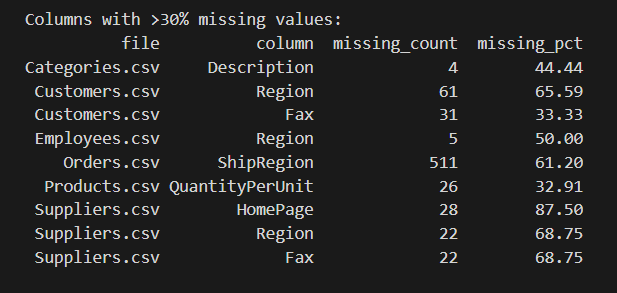
\includegraphics[width=0.7\linewidth,
		height=0.3\textheight,
		keepaspectratio]{phase1_1.png}
		\caption{  گزارش ستون‌های دارای بیش از ۳۰ درصد مقادیر گمشده در هر جدول}
		\label{fig:phase1_1}
	\end{figure}
	
	
	پس از شناسایی درصد مقادیر گمشده در تمامی ستون‌ها، ستون‌هایی که بیش از ۳۰ درصد داده گمشده داشتند به‌صورت جداگانه استخراج شدند تا مطابق الزامات پروژه، وضعیت آن‌ها به‌طور دقیق بررسی شود. برای این منظور، درصد مقادیر گمشده هر ستون محاسبه و تنها ستون‌هایی که از آستانه تعیین‌شده عبور کرده بودند در قالب یک گزارش مجزا نمایش داده شدند. این کار باعث شد تمرکز فرآیند پاک‌سازی بر ستون‌هایی قرار گیرد که بیشترین تأثیر را بر کیفیت داده‌ها دارند و نیازمند تصمیم‌گیری درباره حذف یا جایگزینی مقادیر هستند. در ادامه، برای رفع مقادیر گمشده موجود در ستون توضیحات\LTRfootnote{Description} جدول دسته‌بندی‌ها\LTRfootnote{Categories}، به‌جای استفاده از روش‌های عمومی مانند حذف داده یا جایگزینی با مقادیر ثابت، از توضیحات استاندارد ارائه‌شده در مستندات رسمی پایگاه داده نورث‌ویند استفاده شد. ابتدا نام دسته‌ها به‌منظور جلوگیری از خطاهای ناشی از فاصله‌های اضافی استانداردسازی گردید و سپس تنها ردیف‌هایی که مقدار توضیح آن‌ها خالی بود تکمیل شدند. با این رویکرد، اطلاعات معتبر حفظ شد، از بازنویسی داده‌های صحیح جلوگیری گردید و مقادیر گمشده بر اساس منطق کسب‌وکار و یک منبع معتبر جایگزین شدند.

	\begin{latin}
		\begin{lstlisting}[language=Python]
official_docs_mapping = {'Beverages': 'Soft drinks, coffees, teas, beers, and ales',
	'Condiments': 'Sweet and savory sauces, relishes, spreads, and seasonings',
	'Confections': 'Desserts, candies, and sweet breads',
	'Dairy Products': 'Cheeses',
	'Grains/Cereals': 'Breads, crackers, pasta, and cereal',
	'Meat/Poultry': 'Prepared meats',
	'Produce': 'Dried fruit and bean curd',
	'Seafood': 'Seaweed and fish'}
			
		\end{lstlisting}
	\end{latin}
	
	پس از شناسایی مقادیر گمشده، ستون‌های متنی جداول مشتریان، کارکنان، سفارش‌هاو تأمین‌کنندگان\LTRfootnote{Suppliers} که اطلاعات توصیفی کاربران، کارکنان، سفارش‌ها و تأمین‌کنندگان را نگهداری می‌کنند، مورد بررسی قرار گرفتند. با توجه به ماهیت این ستون‌ها، حذف رکوردها یا استفاده از روش‌های آماری مانند میانگین و میانه برای جایگزینی مقادیر گمشده منطقی نبود؛ زیرا این روش‌ها تنها برای داده‌های عددی کاربرد دارند و می‌توانند موجب از بین رفتن اطلاعات یا ایجاد مقادیر نامعتبر شوند. به همین دلیل، بر اساس مفهوم هر ستون از مقادیر جایگزین معنادار استفاده شد؛ به‌طوری‌که مقدار \lr{Unknown} برای ستون‌های \lr{Region} و \lr{ShipRegion}، مقدار \lr{No Fax} برای ستون \lr{Fax} و مقدار \lr{No Website} برای ستون \lr{HomePage} در نظر گرفته شد. این مقادیر نشان می‌دهند که اطلاعات مربوطه در منبع اولیه ثبت نشده است و با مقادیر واقعی اشتباه گرفته نخواهند شد.
	
	به‌منظور اطمینان از صحت عملیات، تعداد مقادیر گمشده هر ستون قبل و بعد از جایگزینی محاسبه و مقایسه شد تا مشخص شود تمامی مقادیر هدف به‌درستی تکمیل شده‌اند. در پایان نیز فایل‌های اصلاح‌شده ذخیره شدند تا در مراحل بعدی پیش‌پردازش، تحلیل و انتقال داده‌ها به پایگاه داده مورد استفاده قرار گیرند. این رویکرد علاوه بر حفظ تمامی رکوردها، باعث افزایش کیفیت داده‌ها و جلوگیری از بروز خطا در تحلیل‌های بعدی می‌شود.
	
	\begin{figure}[H]
		\centering
		
		% تصویر سمت راست
		\begin{minipage}{0.48\textwidth}
			\centering
			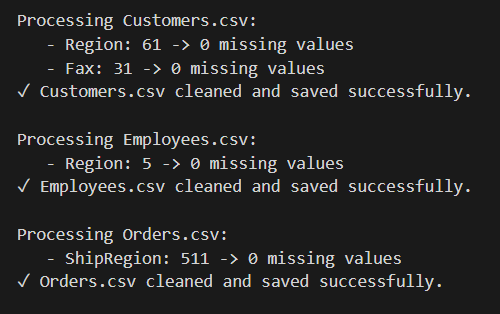
\includegraphics[width=1\linewidth,
			height=0.2\textheight]{phase1_2.png}
			\caption{گزارش پاک‌سازی ستون‌های متنی با جایگزینی مقادیر گمشده به‌صورت معنادار 
				(مانند \lr{Unknown} و \lr{No Fax})}
			\label{fig:hase1_2}
		\end{minipage}
		\hfill % ایجاد فاصله بین دو تصویر
		% تصویر سمت چپ
		\begin{minipage}{0.48\textwidth}
			\centering
			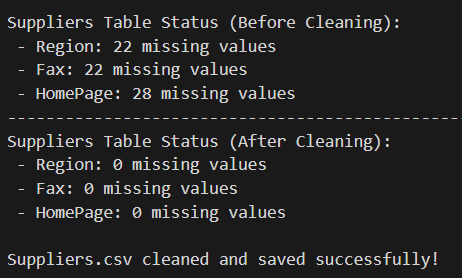
\includegraphics[width=1\linewidth,
			height=0.2\textheight]{phase1_3.png}
			\caption{گزارش پاک‌سازی ستون‌های متنی با جایگزینی مقادیر گمشده به‌صورت معنادار 
				(مانند \lr{Unknown} و \lr{No Fax})}
			\label{fig:phase1_3}
		\end{minipage}
		
	\end{figure}
	
	
	در جدول محصولات\LTRfootnote{Products} نیز ستون \lr{QuantityPerUnit} دارای مقادیر گمشده بود. از آنجا که این ستون نحوه بسته‌بندی یا واحد عرضه هر محصول را توصیف می‌کند و یک ویژگی متنی محسوب می‌شود، جایگزینی آن با مقادیر آماری یا حذف رکوردها مناسب نبود. بنابراین، برای حفظ تمامی محصولات و مشخص بودن وضعیت اطلاعات ناقص، مقادیر گمشده این ستون با عبارت \lr{Not Specified} جایگزین شد. این مقدار نشان می‌دهد که اطلاعات مربوط به نحوه بسته‌بندی محصول در داده‌های اولیه ثبت نشده است، بدون آنکه مفهوم نادرستی به داده اضافه شود.
	
	\begin{figure}[H]
		\centering
		% به جای picture5.png نام عکس واقعی خود را قرار دهید
		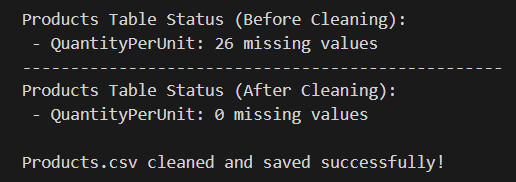
\includegraphics[width=0.7\linewidth,
		height=0.3\textheight,
		keepaspectratio]{phase1_4.png}
		\caption{ تعداد مقادیر گمشده قبل و بعد اصلاح}
		\label{fig:phase1_4}
	\end{figure}
	
	در مرحله بعد، عملیات استانداردسازی روی تمامی ستون‌های متنی انجام شد. این عملیات شامل حذف فاصله‌های اضافی ابتدا و انتهای متن، تبدیل چند فاصله متوالی به یک فاصله، یکسان‌سازی قالب نگارش متن و تبدیل رشته‌هایی مانند \lr{Nan}، \lr{None} و مقادیر خالی به مقدار استاندارد \lr{NA} بود. با این حال، برخی ستون‌ها مانند شناسه‌ها (\lr{CustomerID} و \lr{CustomerTypeID})، تاریخ‌ها، مسیر تصاویر (\lr{PhotoPath})، آدرس صفحات وب (\lr{HomePage}) و داده‌های دودویی تصاویر از این فرآیند مستثنی شدند؛ زیرا تغییر قالب آن‌ها می‌توانست موجب از بین رفتن اطلاعات یا ایجاد ناسازگاری در داده‌ها شود. در پایان، نسخه استانداردشده تمامی جداول ذخیره شد تا داده‌ها از نظر قالب نوشتاری یکدست، سازگار و آماده ورود به مراحل بعدی تحلیل و بارگذاری در پایگاه داده باشند.
	
	\begin{latin}
		\begin{lstlisting}[language=Python]
def normalize_text(df):
text_cols = df.select_dtypes(include=['object']).columns
exclude_cols = ['Picture', 'Photo',
'CustomerID', 'CustomerTypeID',
'BirthDate', 'HireDate', 'OrderDate',
'RequiredDate', 'ShippedDate',
'HomePage', 'PhotoPath']
for col in text_cols:
if col in exclude_cols:
continue
df[col] = df[col].astype(str).str.strip()
df[col] = df[col].str.replace(r'\s+', ' ', regex=True)
df[col] = df[col].str.title()
df[col] = df[col].replace({
	'': pd.NA,
	'Nan': pd.NA,
	'None': pd.NA,
	'<Na>': pd.NA})
return df
		\end{lstlisting}
	\end{latin}
	
	یکی دیگر از مراحل پاک‌سازی داده‌ها، بررسی و حذف ردیف‌های کاملاً تکراری در تمامی جداول پایگاه داده بود. برای افزایش دقت این فرآیند، پیش از مقایسه رکوردها، داده‌های متنی در یک نسخه موقت استانداردسازی شدند؛ به‌طوری‌که تفاوت‌هایی مانند حروف بزرگ و کوچک یا فاصله‌های اضافی در ابتدا و انتهای متن، باعث تشخیص نادرست رکوردهای یکسان نشوند. این استانداردسازی تنها برای فرآیند تشخیص تکراری بودن انجام شد و داده‌های اصلی در این مرحله تغییری نکردند.
	
	در مقابل، برخی ستون‌ها مانند تصاویر، تاریخ‌ها و سایر داده‌هایی که تغییر قالب آن‌ها می‌توانست بر محتوای واقعی اطلاعات تأثیر بگذارد، از فرآیند استانداردسازی مستثنی شدند. پس از شناسایی، تنها نسخه‌های تکراری هر رکورد حذف و اولین نمونه آن حفظ شد. در پایان، تعداد رکوردهای حذف‌شده برای هر جدول گزارش و فایل‌های اصلاح‌شده ذخیره شدند. این فرآیند موجب کاهش افزونگی داده‌ها، حفظ یکپارچگی اطلاعات و جلوگیری از ایجاد خطا در تحلیل‌ها و محاسبات مراحل بعدی شد.
	
	
	\begin{figure}[H]
		\centering
		% به جای picture5.png نام عکس واقعی خود را قرار دهید
		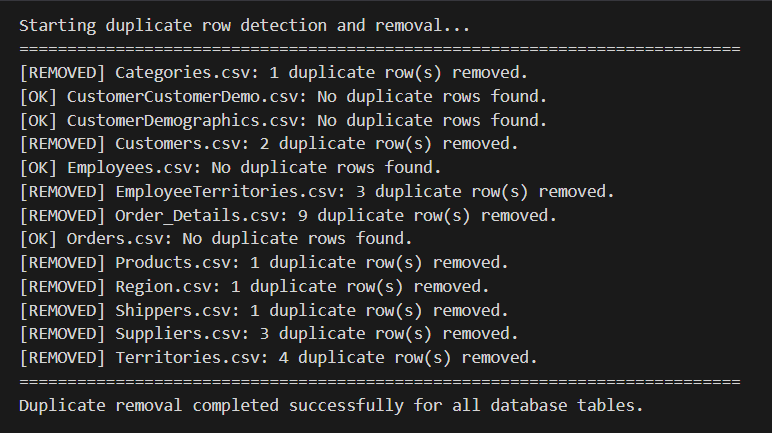
\includegraphics[width=1\linewidth,
		height=0.4\textheight,
		keepaspectratio]{phase1_5.png}
		\caption{ گزارش حذف ردیف‌های کاملاً تکراری از تمام جداول پایگاه داده}
		\label{fig:phase1_5}
	\end{figure}
	
	
	در ادامه فرآیند پاک‌سازی، جدول جزئیات سفارش‌ها\LTRfootnote{Order\_Details} از نظر صحت داده‌های مالی مورد بررسی قرار گرفت. با توجه به اینکه ستون‌های قیمت واحد\LTRfootnote{UnitPrice} و مقدار\LTRfootnote{Quantity} در محاسبه ارزش سفارش‌ها نقش مستقیم دارند، وجود مقادیر صفر یا منفی در این ستون‌ها می‌تواند منجر به ایجاد نتایج نادرست در تحلیل‌های مالی و گزارش‌های مدیریتی شود. به همین دلیل، تمامی رکوردهای جدول از نظر این دو معیار اعتبارسنجی شدند و تعداد ردیف‌های دارای مقادیر نامعتبر شناسایی و گزارش گردید. پس از تکمیل مرحله اعتبارسنجی، رکوردهایی که در آن‌ها مقدار \lr{UnitPrice} یا \lr{Quantity} کمتر یا مساوی صفر بود از مجموعه داده حذف شدند. دلیل انتخاب حذف این رکوردها آن بود که چنین مقادیری از دیدگاه منطق کسب‌وکار فاقد اعتبار هستند و امکان جایگزینی آن‌ها با روش‌های آماری یا مقادیر پیش‌فرض وجود ندارد؛ زیرا هر مقدار جایگزین می‌تواند باعث تحریف محاسبات مالی شود. پس از حذف رکوردهای نامعتبر، تعداد ردیف‌های حذف‌شده محاسبه و جدول اصلاح‌شده ذخیره گردید تا تنها داده‌های معتبر در مراحل بعدی تحلیل، محاسبه ارزش سفارش‌ها و ساخت داشبورد مورد استفاده قرار گیرند.
	
	
	\begin{figure}[H]
		\centering
		% به جای picture5.png نام عکس واقعی خود را قرار دهید
		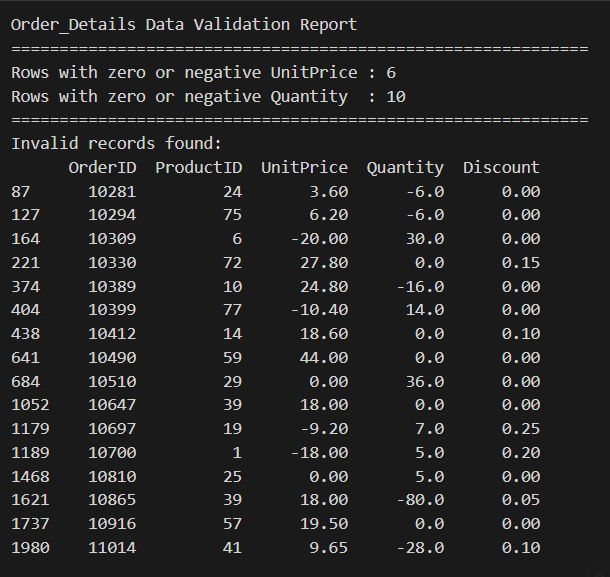
\includegraphics[width=1\linewidth,
		height=0.4\textheight,
		keepaspectratio]{phase1_6.png}
		\caption{  نمایش ردیف هایی با مقادیر صفر یا منفی برای تعداد یا قیمت کالا}
		\label{fig:phase1_6}
	\end{figure}
	
	در ادامه فرآیند پاک‌سازی داده‌ها، ستون‌های متنی جداول مشتریان، کارکنان و تأمین‌کنندگان به‌صورت دقیق‌تری بررسی شدند. علاوه بر مقادیر گمشده استاندارد (\lr{NaN})، رشته‌هایی مانند \lr{"nan"}، \lr{"None"}، \lr{""} و رشته‌های خالی نیز به‌عنوان داده‌های ناقص شناسایی شدند؛ زیرا این مقادیر ممکن است در اثر ورود داده یا تبدیل فایل‌ها به‌صورت متن ذخیره شده باشند و در صورت عدم اصلاح، موجب ناسازگاری در تحلیل داده‌ها یا بارگذاری در پایگاه داده شوند. به همین دلیل، تمامی این نمایش‌های مختلف به‌عنوان یک نوع داده گمشده در نظر گرفته شدند تا فرآیند تکمیل داده‌ها به‌صورت یکنواخت و استاندارد انجام شود.
	
	برای هر ستون، مقدار جایگزین متناسب با مفهوم آن انتخاب شد تا ضمن حفظ معنای اطلاعات، مشخص باشد که مقدار اولیه در داده‌های اصلی وجود نداشته است. به‌عنوان نمونه، در ستون‌های \lr{Region}، \lr{ContactTitle}، \lr{ContactName} و \lr{City} از مقدار \lr{Unknown}، در ستون \lr{Fax} از \lr{No Fax}، در \lr{HomePage} از \lr{No Website}، در \lr{PhotoPath} از \lr{No Path Available} و در \lr{Notes} از \lr{No Notes Available} استفاده شد. همچنین در جدول کارکنان، ستون \lr{ReportsTo} بر اساس ساختار سازمانی تکمیل شد؛ به‌طوری‌که مقدار $0$ برای کارکنانی که سرپرست بالادستی نداشتند در نظر گرفته شد تا جایگاه مدیر ارشد سازمان\LTRfootnote{Top-Level Executive} مشخص باشد. علاوه بر این، ستون تصویر\LTRfootnote{Photo} به دلیل نگهداری داده‌های باینری و نداشتن کاربرد در تحلیل داده‌ها، ساخت داشبوردهای پاور بی‌آی\LTRfootnote{Power BI} و طراحی پایگاه داده حذف گردید. پس از اعمال تمامی اصلاحات، فایل‌های به‌روزشده ذخیره و نتایج عملیات ثبت شدند تا مجموعه داده از نظر یکپارچگی، سازگاری و آمادگی برای مراحل بعدی پردازش در وضعیت مناسبی قرار گیرد.
	
	
	\begin{figure}[H]
		\centering
		% به جای picture5.png نام عکس واقعی خود را قرار دهید
		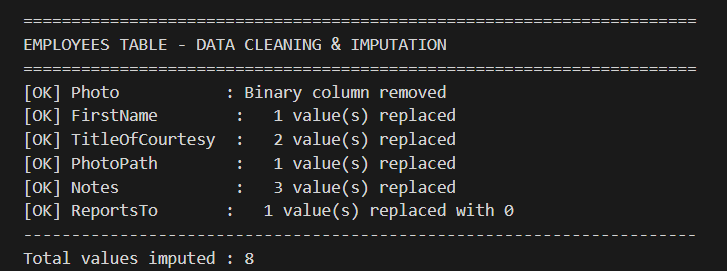
\includegraphics[width=0.8\linewidth,
		height=0.2\textheight,
		keepaspectratio]{phase1_7.png}
		\caption{ پاکسازی و اصلاح کامل تمام مقادیر جدول کارمندان}
		\label{fig:phase1_7}
	\end{figure}
	
	در جدول \lr{Order\_Details}، ستون‌های عددی دارای مقدار گمشده با استفاده از یک رویکرد آماری بررسی و تکمیل شدند. ابتدا ستون تخفیف\LTRfootnote{Discount} به‌دلیل ماهیت داده و منطق کسب‌وکار با مقدار $0.0$ جایگزین شد؛ زیرا نبود مقدار تخفیف به این معناست که برای آن قلم سفارش تخفیفی اعمال نشده است. برای سایر ستون‌های عددی، شامل \lr{UnitPrice} و \lr{Quantity}، پیش از جایگزینی مقادیر گمشده، شاخص‌های آماری میانگین\LTRfootnote{Mean}، میانه\LTRfootnote{Median} و ضریب چولگی\LTRfootnote{Skewness} محاسبه شدند تا مناسب‌ترین روش تکمیل داده انتخاب شود.
	
	معیار تصمیم‌گیری بر اساس میزان چولگی توزیع داده‌ها بود. در صورتی که قدر مطلق ضریب چولگی از $1$ بیشتر باشد، توزیع داده‌ها دارای چولگی قابل‌توجه در نظر گرفته شده و از میانه برای جایگزینی استفاده شد؛ زیرا این شاخص نسبت به مقادیر پرت مقاومت بیشتری دارد. در غیر این صورت، از میانگین استفاده شد، چرا که در توزیع‌های نسبتاً متقارن نماینده مناسبی برای مرکز داده‌ها محسوب می‌شود. پس از تکمیل مقادیر گمشده، ستون \lr{Quantity} مجدداً به نوع داده عدد صحیح تبدیل شد تا با ماهیت شمارشی این متغیر سازگار باقی بماند. این رویکرد علاوه بر پاسخ‌گویی به الزامات پروژه مبنی بر مقایسه میانگین و میانه، انتخاب روش جایگزینی را بر اساس ویژگی‌های واقعی داده‌ها انجام می‌دهد و از اعمال یک روش ثابت برای تمامی متغیرها جلوگیری می‌کند.
	
	
	\begin{figure}[H]
		\centering
		% به جای picture5.png نام عکس واقعی خود را قرار دهید
		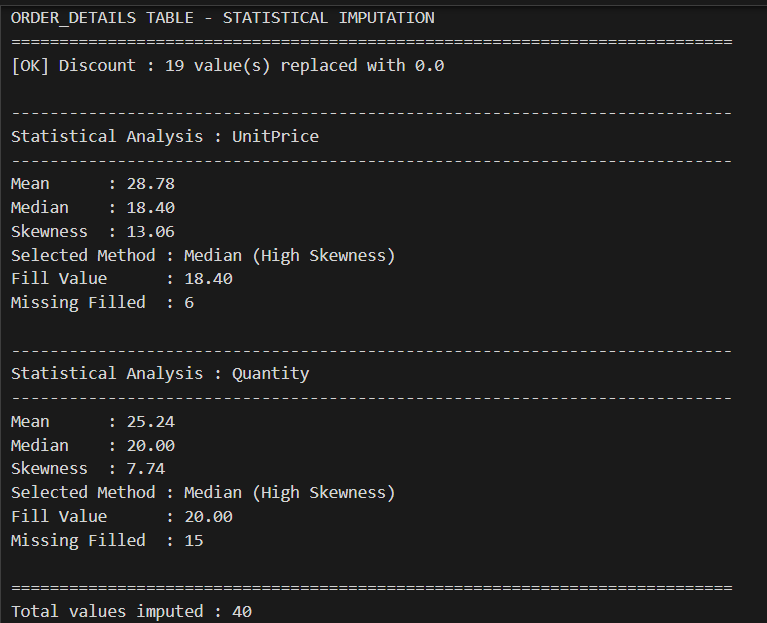
\includegraphics[width=1\linewidth,
		height=0.25\textheight,
		keepaspectratio]{phase1_8.png}
		\caption{ پر کردن ستون تخفیف و مقایسه میانه و میانگین و چولگی ستون های قیمت و تعداد}
		\label{fig:phase1_8}
	\end{figure}
	
	در این مرحله، ستون‌های \lr{OrderDate}، \lr{RequiredDate} و \lr{ShippedDate} در جدول سفارش‌ها به نوع داده زمان‌تاریخ\LTRfootnote{Datetime} تبدیل شدند تا امکان انجام پردازش‌های زمانی، محاسبات تاریخ و تحلیل‌های بعدی در محیط‌های \lr{SQL} و \lr{Power BI} فراهم شود. برای تبدیل تاریخ‌ها از تابع \lr{to\_datetime} با پارامتر \lr{format='mixed'} استفاده شد تا قالب‌های مختلف تاریخ به‌درستی شناسایی شوند. همچنین با استفاده از \lr{errors='coerce'}، مقادیر نامعتبر یا خالی بدون ایجاد خطا به مقدار نامعتبر زمانی\LTRfootnote{NaT: Not a Time} تبدیل شدند. حفظ این مقادیر به‌صورت \lr{NaT} اهمیت دارد؛ زیرا در جدول سفارش‌ها، خالی بودن ستون \lr{ShippedDate} معمولاً نشان‌دهنده سفارش‌هایی است که هنوز ارسال نشده‌اند و این موضوع بخشی از منطق کسب‌وکار محسوب می‌شود، نه یک خطای داده.
	
	\begin{latin}
		\begin{lstlisting}[language=Python]
for col in date_cols:
if col in df.columns:
df[col] = pd.to_datetime(
df[col],
format='mixed',
errors='coerce'
)
nat_count = int(df[col].isna().sum())
print(f"[OK] {col:<15}: Converted to datetime64[ns] | NaT = {nat_count}")
else:
print(f"[SKIP] {col:<15}: Column not found")
		\end{lstlisting}
	\end{latin}
	
	علاوه بر این، ستون کد پستی مقصد\LTRfootnote{ShipPostalCode} از نظر مقادیر گمشده بررسی شد و تمامی مقادیر خالی با مقدار \lr{Unknown} جایگزین شدند تا نمایش داده‌های ناقص در این ستون به‌صورت یکنواخت استاندارد شود. در پایان، فایل اصلاح‌شده ذخیره شد تا ساختار داده‌ها از نظر نوع داده و یکپارچگی مقادیر برای مراحل بعدی پردازش، طراحی پایگاه داده و ساخت داشبورد آماده باشد.
	\begin{latin}
		\begin{lstlisting}[language=Python]
		
if 'ShipPostalCode' in df.columns:
missing_postal = int(df['ShipPostalCode'].isna().sum())			
df['ShipPostalCode'] = (
df['ShipPostalCode']
.fillna('Unknown')
.astype(str)
.str.strip()
)
print(f"[OK] ShipPostalCode : {missing_postal} value(s) replaced with 'Unknown'")
		\end{lstlisting}
	\end{latin}
	
	پس از اتمام تمامی مراحل پاک‌سازی و تکمیل داده‌ها، یک بررسی نهایی بر روی تمام جداول پایگاه داده انجام شد تا وضعیت مقادیر گمشده در مجموعه داده ارزیابی شود. در این مرحله، تعداد و درصد مقادیر گمشده برای تمامی ستون‌های هر جدول مجدداً محاسبه و گزارش شد. هدف از این بررسی، اطمینان از اثربخشی عملیات پاک‌سازی و شناسایی ستون‌هایی بود که ممکن است همچنان دارای داده‌های ناقص باشند. نتایج این ارزیابی به‌عنوان یک مرحله کنترل کیفیت\LTRfootnote{Quality Assurance} مورد استفاده قرار گرفت و امکان مقایسه وضعیت داده‌ها قبل و بعد از عملیات پیش‌پردازش را فراهم کرد. انجام این بررسی نهایی باعث شد اطمینان حاصل شود که داده‌ها از نظر کامل بودن اطلاعات، سازگاری ساختاری و آمادگی برای ورود به مراحل بعدی پروژه، از جمله طراحی پایگاه داده، تحلیل داده و ساخت داشبوردهای \lr{Power BI}، در وضعیت مناسبی قرار دارند.
	
	پس از اتمام عملیات پاک‌سازی داده‌ها، نوع داده تمامی ستون‌های موجود در جداول پایگاه داده مورد بررسی قرار گرفت تا از سازگاری آن‌ها با مفهوم واقعی داده و همچنین الزامات ورود به پایگاه داده‌های مایکروسافت اکسس\LTRfootnote{Microsoft Access} و \lr{SQL Server} اطمینان حاصل شود. در این مرحله، گزارشی از نوع داده هر ستون تهیه شد تا ستون‌هایی که نوع داده آن‌ها با ماهیت اطلاعات ذخیره‌شده مطابقت نداشت، شناسایی شوند. این بررسی نقش یک مرحله کنترل کیفیت را داشت و مبنای انجام اصلاحات لازم در ساختار داده‌ها قرار گرفت. 
	
	بر اساس نتایج این بررسی، نوع داده تعدادی از ستون‌ها استانداردسازی شد. ستون‌های \lr{OrderDate}، \lr{RequiredDate} و \lr{ShippedDate} در جدول سفارش‌ها و همچنین ستون‌های \lr{BirthDate} و \lr{HireDate} در جدول کارکنان به نوع زمان‌تاریخ\LTRfootnote{Datetime} تبدیل شدند تا امکان انجام پردازش‌های زمانی، فیلترهای مبتنی بر تاریخ و تحلیل‌های زمانی در مراحل بعدی فراهم شود.
	
	\begin{figure}[H]
		\centering
		% به جای picture5.png نام عکس واقعی خود را قرار دهید
		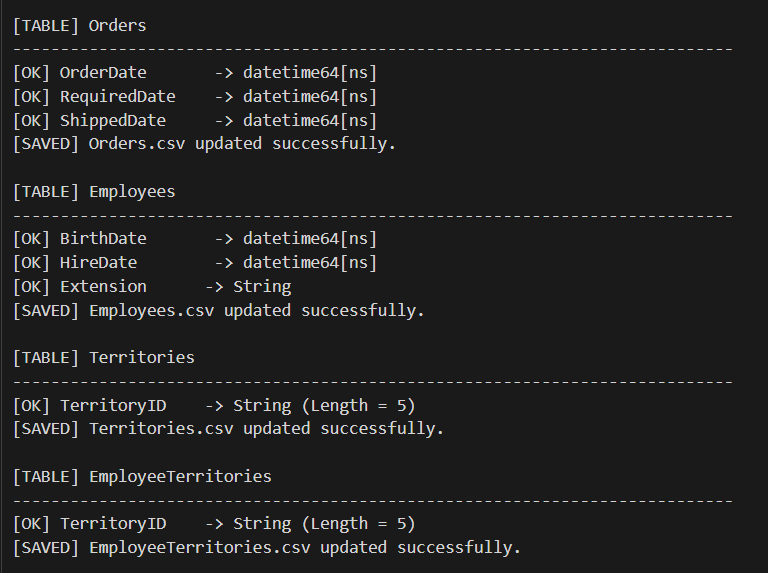
\includegraphics[width=1\linewidth,
		height=0.3\textheight,
		keepaspectratio]{phase1_9.png}
		\caption{ استاندار سازی ستون های ذکر شده}
		\label{fig:phase1_9}
	\end{figure}
	
	
	علاوه بر این، ستون افزونه\LTRfootnote{Extension} در جدول کارکنان که ماهیتی شناسه‌ای و متنی دارد، از نوع عددی به رشته\LTRfootnote{String} تبدیل شد تا صفرهای ابتدایی یا قالب اصلی آن حفظ شود. همچنین ستون \lr{TerritoryID} در جداول \lr{Territories} و \lr{EmployeeTerritories} به رشته تبدیل و با استفاده از صفرهای ابتدایی تا طول پنج کاراکتر استانداردسازی شد. این کار باعث شد قالب کلید اصلی و کلید خارجی در هر دو جدول کاملاً یکسان باشد و از بروز ناسازگاری در برقراری ارتباط بین جداول جلوگیری شود. پس از اعمال تمامی اصلاحات، فایل‌های به‌روزشده ذخیره و مجدداً بررسی شدند تا اطمینان حاصل شود نوع داده تمامی ستون‌های اصلاح‌شده با ساختار منطقی پایگاه داده سازگار بوده و مجموعه داده برای استفاده در مراحل بعدی پروژه کاملاً آماده است.
	
	در پایان مرحله استانداردسازی نوع داده‌ها، تمامی ستون‌های شناسه\LTRfootnote{ID} در جداول پایگاه داده از نظر صحت و یکپارچگی مورد بررسی قرار گرفتند. در این بررسی، تمام ستون‌هایی که نام آن‌ها با \lr{ID} پایان می‌یافت شناسایی شدند و از دو جنبه مورد ارزیابی قرار گرفتند: وجود مقادیر گمشده (\lr{Null}) و وجود مقادیر غیرعددی در ستون‌هایی که ماهیت عددی دارند. از آنجا که ستون‌های \lr{CustomerID} و \lr{CustomerTypeID} به‌صورت شناسه‌های متنی طراحی شده‌اند، این دو ستون از بررسی مقادیر غیرعددی مستثنی شدند. برای سایر ستون‌های شناسه، با تبدیل آزمایشی مقادیر به نوع عددی، هرگونه مقدار نامعتبر یا غیرقابل تبدیل شناسایی شد. نتایج این بررسی برای هر جدول به‌صورت جداگانه گزارش گردید تا در صورت وجود هرگونه ناهماهنگی، امکان اصلاح آن فراهم باشد.
	
	\subsection{مهندسی ویژگی‌ها و آماده‌سازی جهت تحلیل}
	در این مرحله، به‌منظور افزایش قابلیت تحلیل داده‌ها و آماده‌سازی مجموعه داده برای طراحی داشبوردهای \lr{Power BI}، چندین ویژگی جدید از اطلاعات موجود در جدول سفارش‌ها استخراج شد. ابتدا ستون‌های زمانی به نوع داده استاندارد تبدیل شدند تا انجام محاسبات زمانی امکان‌پذیر باشد. سپس از تاریخ سفارش، ویژگی‌های سال سفارش\LTRfootnote{OrderYear}، ماه سفارش\LTRfootnote{OrderMonth} و روز هفته\LTRfootnote{OrderDayOfWeek} استخراج شدند. این ویژگی‌ها امکان تحلیل روند سفارش‌ها در بازه‌های زمانی مختلف، مقایسه عملکرد ماهانه و بررسی الگوهای ثبت سفارش در روزهای مختلف هفته را فراهم می‌کنند.
	
	علاوه بر ویژگی‌های زمانی، دو ویژگی جدید نیز با هدف تحلیل عملکرد فرایند ارسال سفارش‌ها ایجاد شد. ویژگی مدت زمان ارسال\LTRfootnote{ShippingDurationDays} مدت‌زمان بین ثبت سفارش و ارسال آن را بر حسب روز محاسبه می‌کند و می‌تواند برای ارزیابی سرعت ارسال کالا مورد استفاده قرار گیرد. همچنین ویژگی وضعیت تحویل\LTRfootnote{Delivery\_Status} با مقایسه تاریخ ارسال واقعی و تاریخ مورد انتظار وضعیت هر سفارش را در دو دسته به‌موقع\LTRfootnote{On-Time} و دارای تأخیر\LTRfootnote{Delayed} طبقه‌بندی می‌کند. این ویژگی یک شاخص کاربردی برای ارزیابی عملکرد فرآیند لجستیک و تحلیل میزان تأخیر در تحویل سفارش‌ها محسوب می‌شود و می‌تواند در گزارش‌ها و داشبوردهای مدیریتی به‌عنوان یکی از شاخص‌های کلیدی عملکرد مورد استفاده قرار گیرد.
	
	\begin{figure}[H]
		\centering
		% به جای picture5.png نام عکس واقعی خود را قرار دهید
		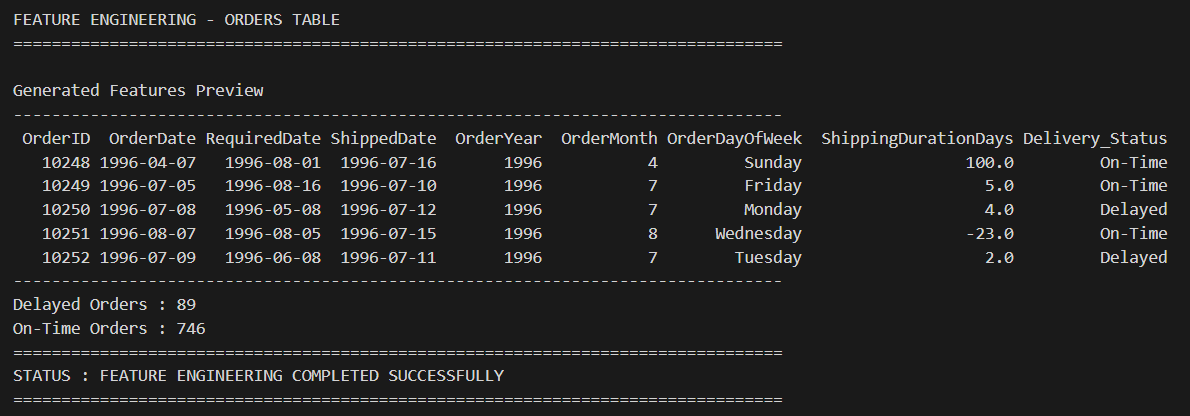
\includegraphics[width=1\linewidth,
		height=0.35\textheight,
		keepaspectratio]{phase1_10.png}
		\caption{ اضافه کردن 5 ستون جدید برای تحلیل راحتتر اطلاعات و طراحی داشبورد}
		\label{fig:phase1_10}
	\end{figure}
	
	در این بخش، ویژگی ارزش سفارش\LTRfootnote{OrderValue} برای هر ردیف از جدول جزئیات سفارش‌ها بر اساس فرمول زیر محاسبه و به مجموعه داده اضافه شد:
		 \lr{OrderValue = UnitPrice * Quantity * (1 - Discount)} 
	این ویژگی ارزش واقعی هر قلم سفارش را پس از اعمال تخفیف نشان می‌دهد و یکی از شاخص‌های اصلی در تحلیل فروش و محاسبه درآمد محسوب می‌شود. همچنین به‌منظور هم‌مقیاس‌سازی متغیرهای عددی، ستون‌های قیمت واحد و مقدار با استفاده از روش مقیاس‌بندی کمینه-بیشینه\LTRfootnote{Min-Max Scaling} نرمال‌سازی شدند. در این روش، مقادیر هر ستون به بازه $0$ تا $1$ تبدیل شدند تا اختلاف مقیاس متغیرها کاهش یابد و امکان مقایسه و تحلیل آن‌ها در مراحل بعدی فراهم شود.
	\vspace{1cm}
	\begin{latin}
		\begin{lstlisting}[language=Python]
df_od['OrderValue'] = (
df_od['UnitPrice'] *
df_od['Quantity'] *
(1 - df_od['Discount'])
)
print("[✔] Feature Created : OrderValue")
		
min_u = df_od['UnitPrice'].min()
max_u = df_od['UnitPrice'].max()
df_od['UnitPrice_Scaled'] = (
(df_od['UnitPrice'] - min_u) /
(max_u - min_u)
)
print("[✔] UnitPrice scaled using Min-Max normalization.")
			
min_q = df_od['Quantity'].min()
max_q = df_od['Quantity'].max()
df_od['Quantity_Scaled'] = (
(df_od['Quantity'] - min_q) /
(max_q - min_q)
)
		\end{lstlisting}
	\end{latin}
	
	در بخش بعد، با ترکیب اطلاعات جداول سفارش‌ها و جزئیات سفارش‌ها، یک جدول جدید با نام ویژگی‌های مشتری\LTRfootnote{Customer\_Features} ایجاد شد که نمایی تجمیع‌شده از رفتار خرید هر مشتری ارائه می‌دهد. برای هر مشتری، تعداد کل سفارش‌ها\LTRfootnote{Total\_Orders}، مجموع هزینه‌کرد\LTRfootnote{Total\_Spend} و میانگین ارزش سفارش\LTRfootnote{Avg\_Order\_Value} محاسبه شد تا شاخص‌های اصلی عملکرد مشتری در یک جدول مستقل در دسترس باشند.
	
	به‌عنوان یک ویژگی تکمیلی، شاخص تازگی خرید\LTRfootnote{Recency\_Days} نیز محاسبه شد که تعداد روزهای سپری‌شده از آخرین خرید هر مشتری را نسبت به آخرین تاریخ ثبت‌شده در مجموعه داده نشان می‌دهد. این شاخص در کنار تعداد سفارش‌ها و میزان هزینه‌کرد، سه مؤلفه اصلی تحلیل تازگی، تکرار و ارزش پولی\LTRfootnote{RFM Analysis} را تشکیل می‌دهد و می‌تواند برای تحلیل رفتار مشتریان، بخش‌بندی آن‌ها و طراحی داشبوردهای مدیریتی مورد استفاده قرار گیرد. در پایان، جدول تولیدشده به‌صورت یک فایل مستقل ذخیره شد تا در مراحل بعدی پروژه قابل استفاده باشد.
	
	
	\begin{figure}[H]
		\centering
		% به جای picture5.png نام عکس واقعی خود را قرار دهید
		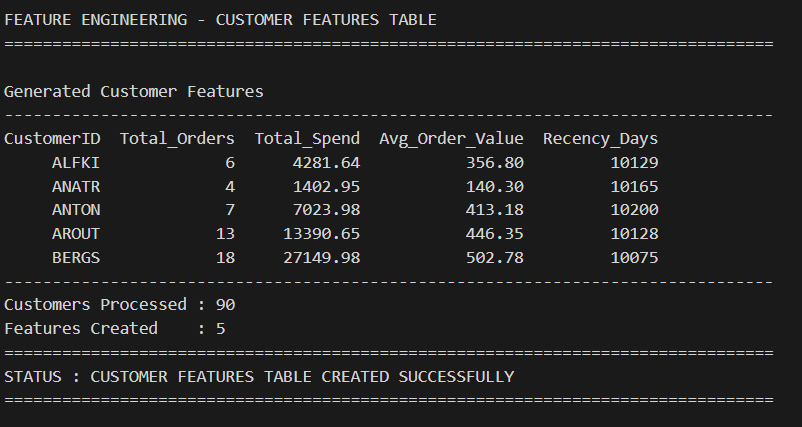
\includegraphics[width=0.7\linewidth,
		height=0.3\textheight,
		keepaspectratio]{phase1_11.png}
		\caption{ساخت جدول ویژگی های مشتری}
		\label{fig:phase1_11}
	\end{figure}
	
	
	ویژگی جدید دسته‌بندی قیمت\LTRfootnote{PriceCategory} برای محصولات ایجاد شد تا کالاها بر اساس قیمت واحد در سه گروه ارزان\LTRfootnote{Low}، متوسط\LTRfootnote{Medium} و گران\LTRfootnote{High} دسته‌بندی شوند. برای این منظور از روش گروه‌بندی مبتنی بر چندک\LTRfootnote{Quantile-Based Binning} استفاده شد که با تقسیم داده‌ها بر اساس چارک‌های آماری، تعداد محصولات را تا حد امکان به‌صورت متوازن میان سه گروه توزیع می‌کند. استفاده از این روش باعث می‌شود دسته‌بندی محصولات به توزیع واقعی قیمت‌ها وابسته باشد و تحت تأثیر انتخاب آستانه‌های دلخواه قرار نگیرد. ویژگی ایجادشده می‌تواند در تحلیل ترکیب سبد محصولات، بررسی الگوی فروش محصولات ارزان و گران‌قیمت و طراحی داشبوردهای مدیریتی مورد استفاده قرار گیرد.
	
	\begin{figure}[H]
		\centering
		% به جای picture5.png نام عکس واقعی خود را قرار دهید
		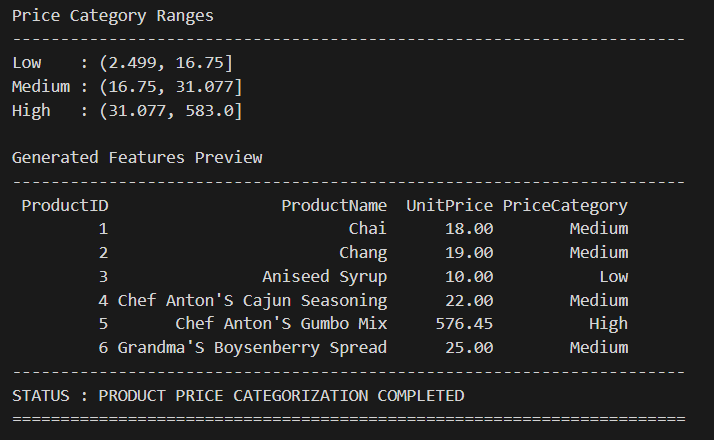
\includegraphics[width=0.7\linewidth,
		height=0.3\textheight,
		keepaspectratio]{phase1_12.png}
		\caption{ ایجاد ستون دسته بندی قیمت ها}
		\label{fig:phase1_12}
	\end{figure}
	
	
	در این بخش، تأثیر نرمال‌سازی با روش مقیاس‌بندی کمینه-بیشینه بر توزیع داده‌های ستون قیمت واحد بررسی شد. برای این منظور، دو شاخص آماری چولگی و کشیدگی\LTRfootnote{Kurtosis} قبل و بعد از نرمال‌سازی محاسبه و با یکدیگر مقایسه شدند تا مشخص شود آیا شکل توزیع داده‌ها دچار تغییر شده است یا خیر. نتایج نشان داد که مقادیر این دو شاخص آماری پس از اعمال نرمال‌سازی تغییری نداشتند. این موضوع نشان می‌دهد که مقیاس‌بندی کمینه-بیشینه تنها مقیاس داده‌ها را به بازه $0$ تا $1$ منتقل می‌کند و به دلیل ماهیت خطی خود، شکل توزیع داده‌ها را حفظ می‌کند. بنابراین، استفاده از این روش باعث استانداردسازی مقیاس متغیرها بدون تغییر ویژگی‌های آماری اصلی آن‌ها می‌شود.
	
	
	\begin{figure}[H]
		\centering
		% به جای picture5.png نام عکس واقعی خود را قرار دهید
		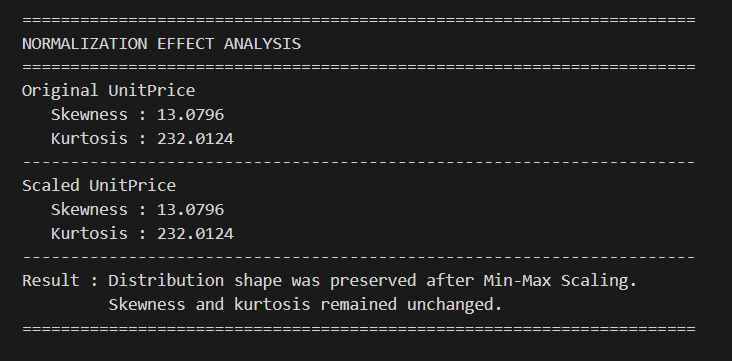
\includegraphics[width=0.7\linewidth,
		height=0.3\textheight,
		keepaspectratio]{phase1_13.png}
		\caption{ مقایسه نرمال سازی داده ها بر چولگی و کشیدگی داده ها}
		\label{fig:phase1_13}
	\end{figure}
	
	
	\subsection{ﺷﻨﺎﺳﺎﻳﻲ ﻭ ﻣﺪﻳﺮﻳﺖ ﺩﺍﺩﻩ ﻫﺎﻱ ﭘﺮﺕ}
	در بخش ابتدایی، هدف اصلی شناسایی و مدیریت داده‌های پرت و غیرمنطقی در جداول مختلف پایگاه داده نورث‌ویند است تا کیفیت داده‌ها برای تحلیل‌های بعدی افزایش یابد. ابتدا همه فایل‌های موردنیاز شامل سفارش‌ها، جزئیات سفارش\LTRfootnote{Order\_Details}، محصولات\LTRfootnote{Products}، تأمین‌کنندگان، دسته‌بندی‌ها و ویژگی‌های مشتریان\LTRfootnote{Customer\_Features} در قالب یک دیکشنری بارگذاری می‌شوند تا دسترسی به آن‌ها ساده‌تر باشد. سپس مقادیر نامعتبر تخفیف\LTRfootnote{Discount} در جدول جزئیات سفارش که خارج از بازه منطقی صفر تا یک هستند، به مقدار گمشده\LTRfootnote{NA} تبدیل می‌شوند. در جدول سفارش‌ها، هزینه حمل\LTRfootnote{Freight} منفی با قدرمطلق‌گیری اصلاح می‌شود، زیرا هزینه حمل نمی‌تواند مقدار منفی داشته باشد. همچنین در جدول محصولات، مقادیر منفی مربوط به موجودی کالا\LTRfootnote{UnitsInStock}، تعداد سفارش‌داده‌شده\LTRfootnote{UnitsOnOrder} و سطح سفارش مجدد\LTRfootnote{ReorderLevel} به صفر تبدیل می‌شوند، چون این مقادیر از نظر عملیاتی نباید منفی باشند. در جدول ویژگی‌های مشتریان نیز تعداد سفارش‌ها\LTRfootnote{Total\_Orders} و مجموع خرید یا هزینه کل مشتری\LTRfootnote{Total\_Spend} اگر صفر یا منفی باشند، به‌عنوان داده نامعتبر شناسایی و با مقدار گمشده جایگزین می‌شوند. در پایان، کد با تعریف چند بررسی کنترلی\LTRfootnote{checks} اطمینان می‌دهد که خطاهای منطقی باقی نمانده‌اند و در صورت پاک بودن داده‌ها، وضعیت پاک بودن داده‌ها\LTRfootnote{Status: Clean} گزارش می‌شود.
	
	\begin{figure}[H]
		\centering
		% به جای picture5.png نام عکس واقعی خود را قرار دهید
		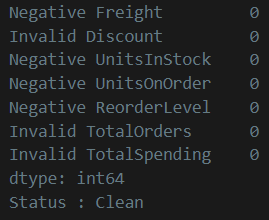
\includegraphics[width=1\linewidth,
		height=0.2\textheight,
		keepaspectratio]{phase1_14.png}
		\caption{ آغاز مرحله پاکسازی داده}
		\label{fig:phase1_14}
	\end{figure}
	
	
	
	در ادامه، داده‌های پرت برای سه ستون قیمت واحد\LTRfootnote{UnitPrice}، تعداد سفارش\LTRfootnote{Quantity} و هزینه حمل بررسی می‌شوند. برای هر ستون، ابتدا مقادیر گمشده حذف شده و سپس با استفاده از روش فاصله بین چارکی\LTRfootnote{IQR}، حدود پایین و بالای قابل‌قبول محاسبه می‌شود. مقادیری که خارج از این محدوده قرار بگیرند، به‌عنوان داده پرت\LTRfootnote{Outlier} شناسایی و تعداد آن‌ها در خروجی چاپ می‌شود. در نهایت، برای هر ستون یک نمودار جعبه‌ای\LTRfootnote{Boxplot} رسم می‌شود تا پراکندگی داده‌ها و نقاط پرت به‌صورت بصری قابل مشاهده و مقایسه باشد.
	
	
	\begin{figure}[H]
		\centering
		% به جای picture5.png نام عکس واقعی خود را قرار دهید
		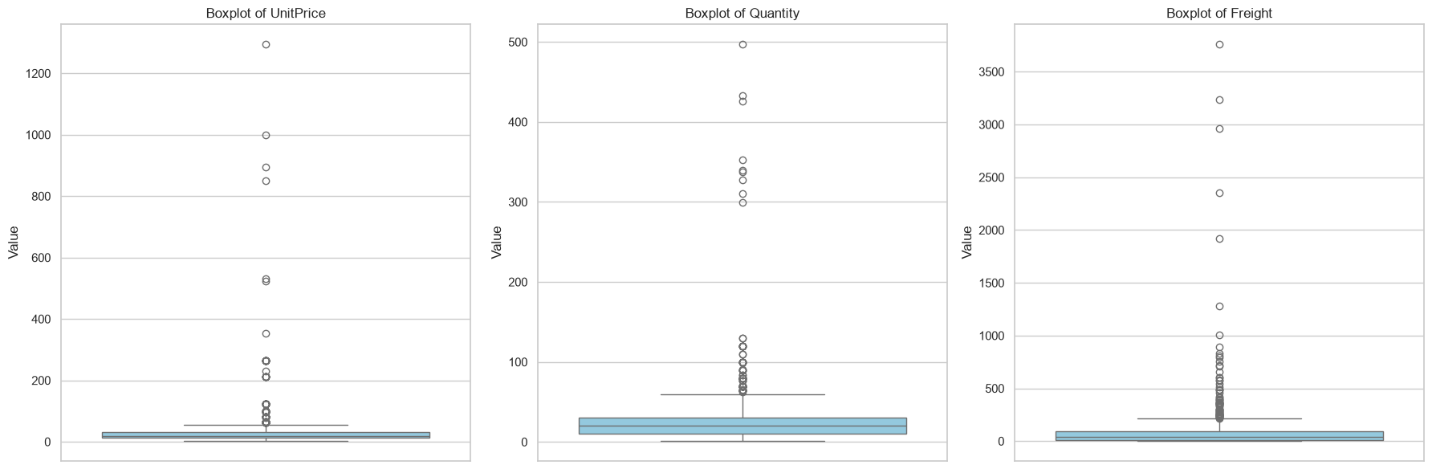
\includegraphics[width=1\linewidth,
		height=0.15\textheight,
		keepaspectratio]{phase1_15.png}
		\caption{نمودار جعبه‌ای}
		\label{fig:phase1_15}
	\end{figure}
	
	
	برای مقایسه شناسایی داده‌های پرت\LTRfootnote{Outliers}، دو روش فاصله بین چارکی\LTRfootnote{IQR} و امتیاز استاندارد\LTRfootnote{Z-Score} در نظر گرفته شده است. در این بررسی، ستون‌های عددی مهم از جداول جزئیات سفارش، سفارش‌ها، محصولات و ویژگی‌های مشتریان انتخاب می‌شوند. ابتدا داده‌ها به قالب عددی تبدیل شده و مقادیر نامعتبر یا گمشده حذف می‌شوند تا نتایج قابل اعتمادتر باشند. سپس در روش فاصله بین چارکی\LTRfootnote{IQR}، مقادیر خارج از محدوده چارک اول و سوم به‌عنوان داده پرت شناسایی می‌شوند. در روش امتیاز استاندارد\LTRfootnote{Z-Score} نیز مقادیری که بیش از سه انحراف معیار از میانگین فاصله دارند، پرت محسوب می‌شوند. در نهایت، تعداد داده‌های پرت شناسایی‌شده با هر دو روش در قالب یک جدول مقایسه‌ای نمایش داده می‌شود تا تفاوت حساسیت این دو رویکرد در ستون‌های مختلف مشخص شود.
	
	
	
	\begin{figure}[H]
		\centering
		% به جای picture5.png نام عکس واقعی خود را قرار دهید
		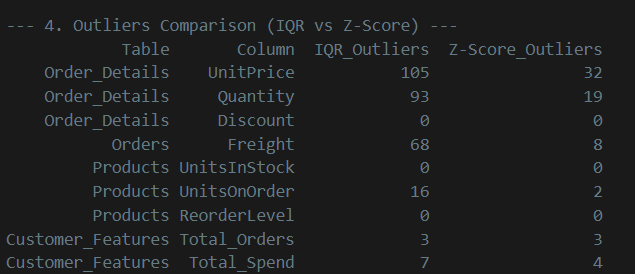
\includegraphics[width=1\linewidth,
		height=0.2\textheight,
		keepaspectratio]{phase1_16.png}
		\caption{مقایسه داده های پرت از دو روش دامنه بین‌چارکی و امتیاز استاندارد }
		\label{fig:phase1_16}
	\end{figure}
	
	برای اجرای روش وینزوریزه کردن\LTRfootnote{Winsorizing}، ستون هزینه حمل از جدول سفارش‌ها انتخاب شده است. در این روش، به‌جای حذف داده‌های پرت، مقادیر بسیار کوچک و بسیار بزرگ در یک بازه مشخص محدود می‌شوند. حد پایین و حد بالا بر اساس صدک‌های ۵ و ۹۵ درصد محاسبه شده و مقادیر خارج از این محدوده با نزدیک‌ترین مقدار مجاز جایگزین می‌شوند. این کار باعث کاهش اثر مقادیر افراطی بر نتایج تحلیل می‌شود، در حالی که ساختار کلی داده‌ها و تعداد رکوردها حفظ می‌گردد. در پایان، توزیع هزینه حمل قبل و بعد از وینزوریزه کردن با هیستوگرام مقایسه می‌شود تا تغییرات ایجادشده به‌صورت بصری قابل مشاهده باشد.
	
	
	\begin{figure}[H]
		\centering
		% به جای picture5.png نام عکس واقعی خود را قرار دهید
		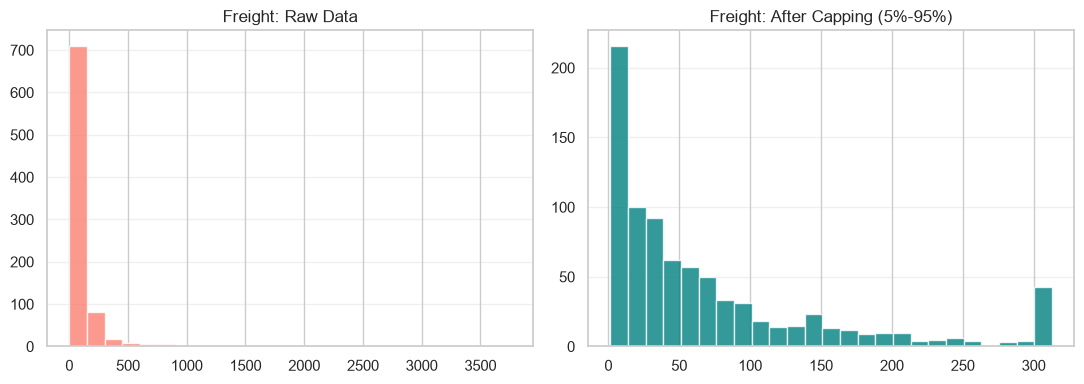
\includegraphics[width=1\linewidth,
		height=0.2\textheight,
		keepaspectratio]{phase1_17.png}
		\caption{مقایسه وضعیت داده های ستون \lr{Freight} قبل و بعد از وينزوريزه کردن  }
		\label{fig:phase1_17}
	\end{figure}
	
	
	برای بررسی وجود سفارش‌هایی با تعداد بسیار زیاد، ستون تعداد سفارش در جدول جزئیات سفارش تحلیل می‌شود. در این بررسی، ابتدا حدود نرمال داده‌ها با استفاده از روش فاصله بین چارکی محاسبه شده و سپس سفارش‌هایی که مقدار تعداد آن‌ها از حد بالای نرمال بیشتر باشد، به‌عنوان سفارش‌های غیرعادی شناسایی می‌شوند. علاوه بر شمارش این موارد، ده مقدار بزرگ‌تر ستون تعداد نیز نمایش داده می‌شود تا شدت مقادیر بالا بهتر قابل بررسی باشد. نمودار جعبه‌ای\LTRfootnote{Boxplot} نیز برای مشاهده دیداری پراکندگی داده‌ها و تشخیص نقاط پرت استفاده می‌شود.
	
	برای بررسی قیمت‌های غیرعادی محصولات، ستون قیمت واحد در جدول محصولات مورد ارزیابی قرار می‌گیرد. در این بخش، حد پایین و حد بالا بر اساس روش فاصله بین چارکی تعیین می‌شود و محصولاتی که قیمت آن‌ها کمتر یا بیشتر از این بازه باشد، به‌عنوان قیمت غیرعادی پایین یا بالا شناسایی می‌شوند. سپس تعداد موارد غیرعادی گزارش شده و ده قیمت بالاتر و ده قیمت پایین‌تر محصولات نمایش داده می‌شود. در پایان، نمودار جعبه‌ای قیمت محصولات رسم می‌شود تا وجود قیمت‌های پرت و الگوی توزیع قیمت‌ها به‌صورت بصری قابل مشاهده باشد.
	
	
	\begin{figure}[H]
		\centering
		
		% تصویر سمت راست
		\begin{minipage}{0.48\textwidth}
			\centering
			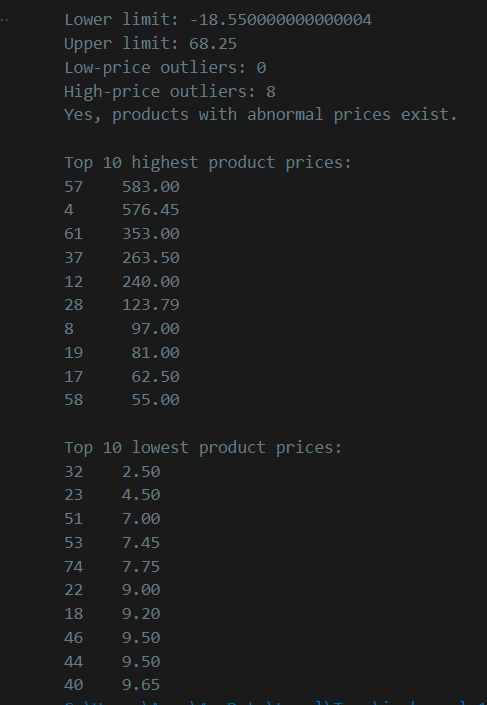
\includegraphics[width=1\linewidth,
			height=0.2\textheight]{phase1_18.png}
			\caption{قیمت های بسیار پایین یا بالا}
			\label{fig:hase1_18}
		\end{minipage}
		\hfill % ایجاد فاصله بین دو تصویر
		% تصویر سمت چپ
		\begin{minipage}{0.48\textwidth}
			\centering
			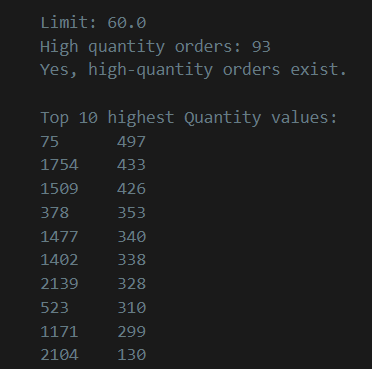
\includegraphics[width=1\linewidth,
			height=0.2\textheight]{phase1_19.png}
			\caption{مقادیر بسیار بالا برای تعداد}
			\label{fig:phase1_19}
		\end{minipage}
		
	\end{figure}
	
	در این بخش، اثر حذف داده‌های پرت بر شاخص‌های آماری اصلی مانند میانگین و انحراف معیار\LTRfootnote{Standard Deviation} بررسی می‌شود. ابتدا ستون‌های عددی مهم از جداول جزئیات سفارش، سفارش‌ها، محصولات و ویژگی‌های مشتریان انتخاب می‌شوند و داده‌های آن‌ها به قالب عددی تبدیل می‌گردند. سپس برای هر ستون، داده‌های پرت با استفاده از روش فاصله بین چارکی شناسایی و از مجموعه داده کنار گذاشته می‌شوند. پس از حذف مقادیر پرت، میانگین و انحراف معیار قبل و بعد از حذف محاسبه و با یکدیگر مقایسه می‌شوند. در پایان، میزان تغییر میانگین، تغییر انحراف معیار و تعداد داده‌های حذف‌شده در قالب یک جدول خلاصه نمایش داده می‌شود تا مشخص شود داده‌های پرت چه اثری بر توزیع و پراکندگی داده‌ها داشته‌اند.
	
	\begin{figure}[H]
		\centering
		% به جای picture5.png نام عکس واقعی خود را قرار دهید
		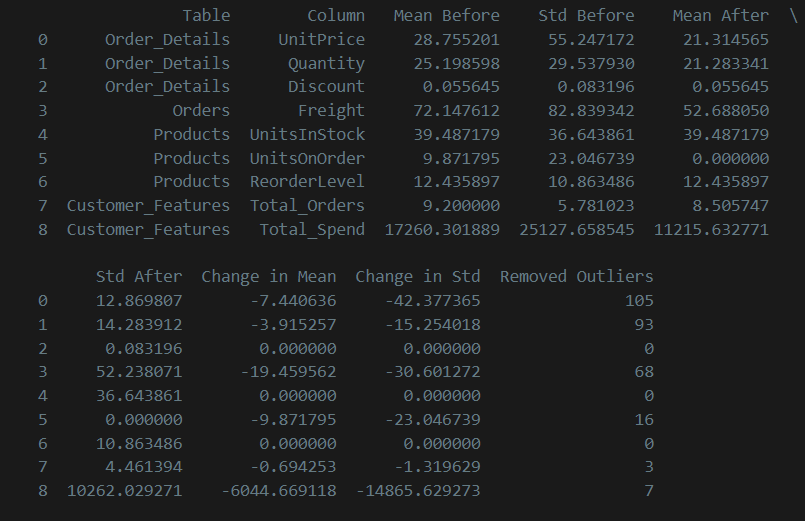
\includegraphics[width=1\linewidth,
		height=0.3\textheight,
		keepaspectratio]{phase1_20.png}
		\caption{تغییرات انحراف معیار و میانگین بعد حذف داده پرت  }
		\label{fig:phase1_20}
	\end{figure}
	
	
	منطق مدیریت داده‌های پرت\LTRfootnote{Outlier Management} بر پایه این فرض شکل گرفت که همه مقادیر پرت الزاماً خطا نیستند و نباید صرفاً به دلیل فاصله داشتن از الگوی عمومی داده‌ها حذف شوند. در داده‌های فروش، بسیاری از مقادیر بزرگ یا غیرمعمول می‌توانند بازتاب رخدادهای واقعی کسب‌وکار باشند؛ برای مثال، سفارش‌هایی با تعداد بالا، هزینه حمل زیاد، یا مشتریانی با مجموع خرید چشمگیر، ممکن است دقیقاً همان موارد مهم و ارزشمندی باشند که شناخت آن‌ها برای تحلیل رفتار بازار ضروری است. به همین دلیل، میان «خطاهای فنی»\LTRfootnote{Technical Errors} و «پرت‌های تجاری»\LTRfootnote{Business Outliers} تمایز در نظر گرفته شد.
	
	خطاهای فنی شامل مقادیری هستند که از نظر منطقی یا ساختاری نامعتبرند؛ مانند تخفیف خارج از بازه مجاز، مقادیر منفی در متغیرهایی که نباید منفی باشند، یا ثبت‌های ناسازگار با قواعد داده. این موارد چون بیانگر واقعیت نیستند، در مرحله پاک‌سازی اصلاح یا حذف شدند. اما مقادیری که فقط از نظر آماری در نواحی دورافتاده توزیع قرار دارند، لزوماً نامعتبر تلقی نشدند. برای این دسته، تصمیم بر حفظ رکورد و اضافه‌کردن یک شاخص کمکی اتخاذ شد تا وضعیت پرت بودن آن‌ها مشخص بماند، بدون آن‌که اطلاعات اصلی از بین برود.
	
	برای این منظور، پس از محاسبه حدود نرمال هر متغیر با روش فاصله بین چارکی، رکوردهای خارج از این محدوده شناسایی شدند و برای هر ستون منتخب، یک متغیر بولی\LTRfootnote{Boolean Flag} با عنوان \lr{IsOutlier} ساخته شد. این علامت‌گذاری باعث می‌شود هر مشاهده پرت به‌صورت شفاف مستند شود، در حالی که خود داده همچنان در مجموعه اصلی باقی بماند. بنابراین، تصمیم نهایی درباره استفاده یا عدم استفاده از این رکوردها به مرحله تحلیل منتقل می‌شود، نه این‌که در همان مرحله پاک‌سازی به‌طور برگشت‌ناپذیر حذف شوند.
	
	دلیل پرهیز از حذف آن است که حذف داده‌های پرت در داده‌های تجاری می‌تواند موجب از دست رفتن سیگنال‌های کلیدی و ایجاد سوگیری در نتایج شود. اگر سفارش‌های بزرگ، محصولات با قیمت‌های خاص، یا مشتریان با خرید بالا حذف شوند، تصویری که از واقعیت بازار به‌دست می‌آید، دیگر تصویر کاملی نخواهد بود. در چنین شرایطی، میانگین‌ها و شاخص‌های آماری ممکن است ظاهراً متعادل‌تر شوند، اما این تعادل به بهای حذف بخش مهمی از واقعیت عملیاتی سیستم حاصل می‌شود. از منظر تحلیلی، چنین کاری می‌تواند شناخت مشتریان ارزشمند، الگوهای خرید غیرمعمول و فرصت‌های بالقوه کسب‌وکار را محدود کند.
	
	رویکرد نگهداری همراه با علامت‌گذاری این مزیت را ایجاد می‌کند که در ادامه، هم تحلیل بر مبنای داده‌های عادی ممکن باشد و هم بررسی مستقل روی رکوردهای پرت انجام شود. به بیان دیگر، داده‌های پرت به‌جای آن‌که به‌عنوان «مزاحم» کنار گذاشته شوند، به‌عنوان یک لایه اطلاعاتی مهم حفظ می‌شوند. این کار به تحلیل‌گر اجازه می‌دهد بسته به هدف مطالعه، یا آن‌ها را موقتاً از تحلیل‌های عمومی کنار بگذارد، یا برعکس، به‌صورت ویژه روی آن‌ها تمرکز کند. در نتیجه، فرآیند پاک‌سازی نه‌تنها به کاهش خطا کمک می‌کند، بلکه ظرفیت تحلیلی داده را نیز افزایش می‌دهد. در مجموع، تصمیم نهایی بر حذف نکردن داده‌های پرت، یک انتخاب صرفاً آماری نبود، بلکه انتخابی مبتنی بر منطق مسئله، ماهیت داده‌های فروش و ارزش اطلاعاتی رکوردهای غیرعادی بود. چنین تصمیمی نشان می‌دهد که مدیریت داده‌های پرت زمانی مؤثرتر است که به‌جای حذف شتاب‌زده، بر تشخیص، مستندسازی و استفاده هوشمندانه از آن‌ها تکیه شود.
	
	\subsection{ﺍﻋﺘﺒﺎﺭﺳﻨﺠﻲ ﺩﺍﺩﻩ ﻫﺎ}
	
	در ابتدای بخش ششم، توالی منطقی تاریخ‌های مربوط به سفارش‌ها بررسی شد تا ناسازگاری‌های زمانی در جدول \lr{Orders} شناسایی شوند. ابتدا ستون‌های \lr{OrderDate}، \lr{RequiredDate} و \lr{ShippedDate} به قالب تاریخ تبدیل شدند و مقادیر نامعتبر به‌صورت \lr{NaT} در نظر گرفته شدند. سپس کد بررسی کرد که تاریخ ارسال قبل از تاریخ سفارش نباشد، چون چنین حالتی از نظر فرآیند واقعی سفارش نامعتبر است. همچنین تاریخ موردنیاز نباید زودتر از تاریخ ثبت سفارش باشد، بنابراین این موارد نیز به‌عنوان خطای منطقی شناسایی شدند. برای حفظ سایر اطلاعات مفید سفارش، رکوردها حذف نشدند و فقط مقدارهای تاریخی اشتباه با \lr{NaT} جایگزین شدند. در ادامه، سفارش‌هایی که بعد از تاریخ موردنیاز ارسال شده بودند با ستون \lr{Late\_Shipment} علامت‌گذاری شدند. در نهایت، تعداد روزهای تأخیر در ستون \lr{Delay\_Days} محاسبه شد تا این اطلاعات برای تحلیل عملکرد ارسال‌ها قابل استفاده باشد.
	
	در ابتدا، ستون‌های تاریخ سفارش\LTRfootnote{OrderDate}، تاریخ موردنیاز\LTRfootnote{RequiredDate} و تاریخ ارسال\LTRfootnote{ShippedDate} به فرمت استاندارد زمانی\LTRfootnote{datetime} تبدیل شدند تا امکان مقایسه ریاضی فراهم گردد. در مرحله بعد، سه سناریوی متناقض شامل پیشی گرفتن تاریخ ارسال بر سفارش، پیشی گرفتن تاریخ موردنیاز بر سفارش، و تأخیر ارسال نسبت به تاریخ درخواستی مشتری مورد سنجش قرار گرفتند. برای مدیریت خطاها، تصمیم بر آن شد که در صورت رخ دادن هرگونه تناقض زمانی، مقدار نامعتبر به عنوان داده‌ی مفقودِ ساختاریافته\LTRfootnote{pd.NaT} در نظر گرفته شود. این استراتژی پاک‌سازی تضمین می‌کند که رکوردهای ناسازگار از محاسبات زنجیره تأمین حذف شده و تحلیل‌های لجستیکی و زمان انتظار\LTRfootnote{Lead Time} در مراحل بعدی دچار انحراف محاسباتی نشوند.
	
	\begin{figure}[H]
		\centering
		% به جای picture5.png نام عکس واقعی خود را قرار دهید
		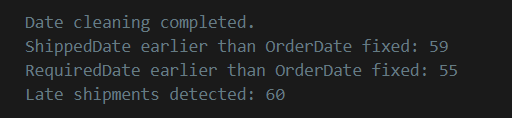
\includegraphics[width=1\linewidth,
		height=0.2\textheight,
		keepaspectratio]{phase1_21.png}
		\caption{پاکسازی تاریخ های نا معتبر و غیرمنطقی }
		\label{fig:phase1_21}
	\end{figure}
	
	
	سپس، هدف حفظ یکپارچگی ارجاعی\LTRfootnote{Referential Integrity} میان جدول جزئیات سفارش\LTRfootnote{Order\_Details} و جدول سفارش‌ها\LTRfootnote{Orders} است؛ یعنی هر شناسه سفارش\LTRfootnote{OrderID} که در جدول جزئیات سفارش ثبت شده، باید در جدول اصلی سفارش‌ها نیز وجود داشته باشد. برای این منظور، ابتدا شناسه‌های سفارش از هر دو جدول استخراج و با یکدیگر مقایسه شدند. سپس شناسه‌هایی که در جدول جزئیات سفارش وجود داشتند اما در جدول سفارش‌ها یافت نشدند، به‌عنوان رکوردهای نامعتبر شناسایی شدند. در مرحله پاک‌سازی، فقط ردیف‌هایی از جدول جزئیات سفارش نگه داشته شدند که شناسه سفارش آن‌ها در جدول سفارش‌ها موجود بود و سایر موارد حذف شدند. همچنین تعداد ردیف‌ها پیش و پس از اصلاح محاسبه شد تا میزان داده‌های حذف‌شده مشخص باشد. اجرای این فرایند باعث می‌شود رابطه میان جدول سفارش‌ها و جزئیات آن‌ها معتبر، سازگار و قابل اتکا باقی بماند و تحلیل‌های بعدی بر پایه داده‌های صحیح انجام شوند.
	
	\begin{figure}[H]
		\centering
		% به جای picture5.png نام عکس واقعی خود را قرار دهید
		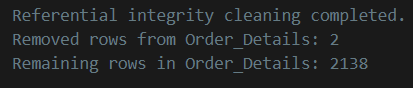
\includegraphics[width=1\linewidth,
		height=0.2\textheight,
		keepaspectratio]{phase1_22.png}
		\caption{بررسی و پاکسازی شناسه‌های بی‌پشتوانه }
		\label{fig:phase1_22}
	\end{figure}
	
در ادامه، هدف شناسایی مقدارهای نامعتبر منطقی در ستون‌هایی است که طبق قواعد کسب‌وکار نباید منفی یا خارج از محدوده مجاز باشند. در جدول جزئیات سفارش بررسی می‌شود که تعداد سفارش بزرگ‌تر از صفر باشد، تخفیف در بازه مجاز صفر تا یک قرار بگیرد و قیمت واحد مقدار منفی نداشته باشد. همچنین در جدول سفارش‌ها هزینه حمل از نظر منفی نبودن کنترل می‌شود. در جدول محصولات نیز موجودی کالا و قیمت واحد محصول بررسی می‌شوند تا مقدار منفی در آن‌ها وجود نداشته باشد. این کد فقط موارد نامعتبر را شناسایی و تعداد آن‌ها را گزارش می‌کند تا مشخص شود کدام بخش‌های داده نیازمند اصلاح یا پاک‌سازی هستند. چنین کنترلی باعث می‌شود داده‌هایی که از نظر منطقی قابل قبول نیستند، پیش از ورود به تحلیل‌های بعدی تشخیص داده شوند.
	
	\begin{figure}[H]
		\centering
		% به جای picture5.png نام عکس واقعی خود را قرار دهید
		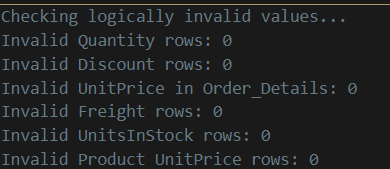
\includegraphics[width=1\linewidth,
		height=0.2\textheight,
		keepaspectratio]{phase1_23.png}
		\caption{بررسی تعداد داده‌های غیرمنطقی منفی برای ستون های عددی همواره بزرگتر از 0 }
		\label{fig:phase1_23}
	\end{figure}
	
	
	به منظور حصول اطمینان از اعتبار ستون تخفیف\LTRfootnote{Discount} و پایبندی به قوانین کسب‌وکار، بازبینی نهایی جهت اطمینان از قرارگیری تمامی مقادیر تخفیف در بازه منطقی $[0, 1]$ انجام شد. از آنجایی که در فازهای ابتدایی پیش‌پردازش، تمامی مقادیر نامعتبر و خارج از این دامنه شناسایی، فیلتر یا اصلاح شده بودند، اجرای این بررسی در این مرحله تنها نقش «تأییدیه نهایی»\LTRfootnote{Re-validation} را داشت. نتایج حاصل از این ارزیابی مؤید آن است که داده‌ها کاملاً پاک‌سازی شده و هیچ‌گونه مقدار غیرمجاز یا ناهنجاری در ستون تخفیف وجود ندارد که بتواند محاسبات سود و تحلیل‌های مالی را در مراحل بعدی دچار خطا کند.
	
	
	\begin{figure}[H]
		\centering
		% به جای picture5.png نام عکس واقعی خود را قرار دهید
		
\includegraphics[width=1\linewidth,
		height=0.2\textheight,
		keepaspectratio]{phase1_24.png}
		\caption{بررسی ناهنجاری ستون تخفیف }
		\label{fig:phase1_24}
	\end{figure}
	
	
	
	حال، هدف در ادامه بررسی یکپارچگی ارجاعی\LTRfootnote{Referential Integrity} میان جدول محصولات و جدول دسته‌بندی‌ها است تا اطمینان حاصل شود هر شناسه دسته‌بندی\LTRfootnote{CategoryID} ثبت‌شده برای یک محصول، واقعاً در جدول دسته‌بندی‌ها وجود دارد. ابتدا وجود جدول دسته‌بندی‌ها در مجموعه داده‌ها کنترل می‌شود و در صورت موجود بودن، شناسه‌های دسته‌بندی محصولات با شناسه‌های معتبر جدول \lr{Categories} مقایسه می‌شوند. محصولاتی که دارای شناسه دسته‌بندی نامعتبر باشند، شناسایی و نمونه‌ای از آن‌ها نمایش داده می‌شود. سپس برای پاک‌سازی، فقط محصولاتی در جدول \lr{Products} نگه داشته می‌شوند که شناسه دسته‌بندی معتبر دارند. تعداد ردیف‌ها قبل و بعد از اصلاح محاسبه می‌شود تا مشخص شود چه تعداد محصول به دلیل دسته‌بندی نامعتبر حذف شده‌اند. این کار باعث می‌شود ارتباط میان محصولات و دسته‌بندی‌ها سازگار باقی بماند و تحلیل‌های مربوط به گروه‌بندی محصولات بر پایه داده‌های معتبر انجام شود.
	\begin{figure}[H]
		\centering
		% به جای picture5.png نام عکس واقعی خود را قرار دهید
		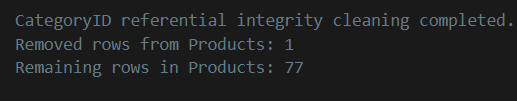
\includegraphics[width=1\linewidth,
		height=0.2\textheight,
		keepaspectratio]{phase1_25.png}
		\caption{بررسی و اصلاح شناسه‌های محصول نامعتبر }
		\label{fig:phase1_25}
	\end{figure}
	
	
	در پایان، برای تهیه گزارش کیفیت داده‌ها، تابعی تعریف شد تا تعداد خطاهای شناسایی‌شده در هر جدول و هر قانون اعتبارسنجی را به‌صورت خلاصه استخراج کند. این تابع با تولید خروجی آماری، امکان مشاهده و مقایسه وضعیت داده‌ها را قبل و بعد از اعمال اصلاحات فراهم می‌سازد. به بیان دیگر، از این گزارش می‌توان برای بررسی میزان خطاهای موجود و ارزیابی اثر پاک‌سازی انجام‌شده استفاده کرد. همچنین جزئیات رکوردهای نامعتبر نیز در خروجی جداگانه نگهداری شد تا در صورت نیاز، پیگیری و بازبینی آن‌ها امکان‌پذیر باشد. در نتیجه، این مرحله به‌عنوان جمع‌بندی نهایی، تصویری روشن از تعداد خطاها و اصلاحات انجام‌شده ارائه می‌دهد.در انتها تمامی تغیرات ایجاد شده بر دیتافریم ها را روی فایل های سی اس وی\LTRfootnote{CSV} اعمال می‌کنیم.
	
	
	\begin{figure}[H]
		\centering
		% به جای picture5.png نام عکس واقعی خود را قرار دهید
		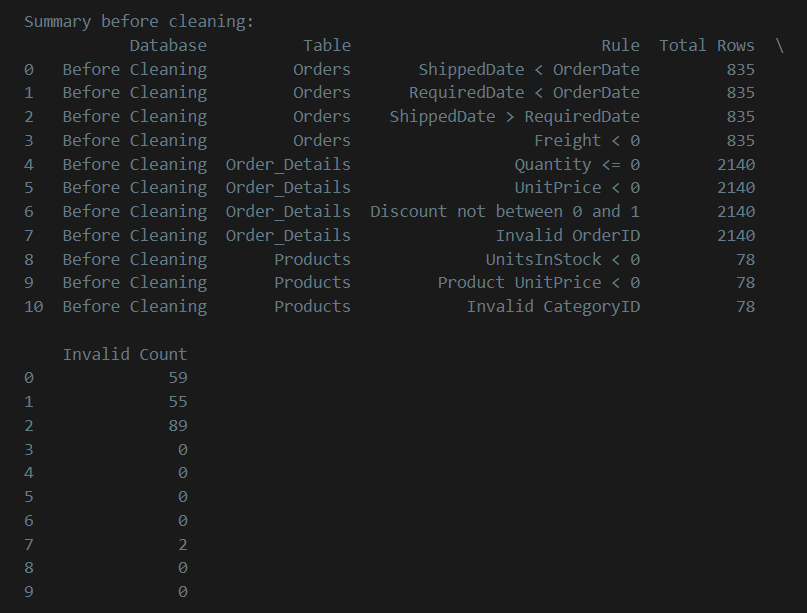
\includegraphics[width=1\linewidth,
		height=0.4\textheight,
		keepaspectratio]{phase1_26.png}
		\caption{وضعیت داده‌ها قبل از اصلاح}
		\label{fig:phase1_26}
	\end{figure}
	
	
		% =======================================================
	% ------------------- فاز دوم پروژه ------------------- %
	% =======================================================
	\newpage
	\section{فاز دوم}
	\subsection{اعتبارسنجی داده‌ها}
	
	در بخش ابتدایی فاز دوم پروژه، با هدف کنترل صحت ورود اطلاعات و جلوگیری از ثبت داده‌های نادرست در انبار، یک فرم ورود اطلاعات کالا در محیط اکسل\LTRfootnote{Microsoft Excel} طراحی شد. این فرم در کاربرگ\LTRfootnote{Sheet} جدول محصولات\LTRfootnote{Product\_Table} ایجاد گردید و برای ساختاردهی بهتر داده‌ها، ابتدا محدوده مورد نظر با استفاده از ابزار درج جدول\LTRfootnote{Insert Table} به یک جدول رسمی در اکسل تبدیل شد. استفاده از جدول\LTRfootnote{Table} باعث شد ستون‌ها دارای عنوان مشخص، فیلتر، قالب‌بندی منظم و قابلیت توسعه خودکار باشند؛ به این معنا که با اضافه شدن رکوردهای جدید، قوانین و قالب جدول نیز به صورت منظم ادامه پیدا کند.
	
	در این فرم، ستون‌های اصلی مورد نیاز برای ثبت اطلاعات کالاها تعریف شدند. این ستون‌ها شامل سریال محصول\LTRfootnote{Product\_Serial}، نام محصول\LTRfootnote{Product\_Name}، دسته‌بندی\LTRfootnote{Category}، کد ردیف انبار\LTRfootnote{Warehouse\_Row\_Code}، تاریخ تولید\LTRfootnote{Production\_Date}، تاریخ تحویل\LTRfootnote{Delivery\_Date}، تعداد واحد\LTRfootnote{Unit\_Quantity}، قیمت واحد\LTRfootnote{Unit\_Price} و تأیید کیفیت\LTRfootnote{Quality\_Approval} هستند. هر یک از این فیلدها مطابق خواسته پروژه برای ثبت یک نوع مشخص از اطلاعات در نظر گرفته شده‌اند و برای جلوگیری از ورود داده‌های اشتباه، روی آن‌ها قوانین اعتبارسنجی اعمال شد.
	
	برای انجام اعتبارسنجی، از ابزار اعتبارسنجی داده‌ها\LTRfootnote{Data Validation} در اکسل استفاده شد. در ستون سریال محصول، ورود سریال کالا به صورت یک کد عددی یکتا تعریف شد و برای راهنمایی کاربر، پیام ورودی مناسب نمایش داده شد؛ به عنوان نمونه، هنگام انتخاب سلول مربوط به سریال کالا، پیام راهنما با عنوان شماره سریال\LTRfootnote{Serial Number} نمایش داده می‌شود و از کاربر خواسته می‌شود یک کد ۸ رقمی یکتا وارد کند. این کار باعث می‌شود کاربر قبل از ورود اطلاعات، با قالب صحیح داده آشنا شود. 
	
	در ستون نام محصول، محدودیت لازم برای ثبت نام کالا در نظر گرفته شد تا مقدار واردشده با ماهیت این فیلد سازگار باشد و از ثبت داده‌های نامعتبر جلوگیری شود. برای ستون دسته‌بندی نیز از فهرست انتخابی استفاده شد تا کاربر بتواند دسته‌بندی کالا را فقط از میان گزینه‌های مجاز انتخاب کند. به همین منظور، یک کاربرگ جداگانه با نام فهرست‌ها\LTRfootnote{Lists} طراحی شد که در آن گزینه‌های مورد نیاز برای فیلدهای فهرستی قرار گرفتند. این کار باعث شد مقادیر انتخابی در فرم اصلی استاندارد باشند و از نوشتن شکل‌های متفاوت یا اشتباه یک دسته‌بندی جلوگیری شود. 
	
	برای ستون کد ردیف انبار نیز قالب مشخصی در نظر گرفته شد تا کد ردیف انبار طبق الگوی خواسته‌شده وارد شود؛ یعنی ترکیبی از یک حرف بزرگ و یک عدد تک‌رقمی باشد. همچنین برای ستون‌های تاریخ تولید و تاریخ تحویل، اعتبارسنجی مربوط به تاریخ اعمال شد تا تاریخ‌ها در قالب معتبر وارد شوند. در مورد تاریخ تحویل، منطق ورود داده به گونه‌ای در نظر گرفته شد که با تاریخ تولید سازگار و بعد از آن باشد و مقدار نامعتبر ثبت نشود. 
	
	در ستون تعداد واحد، ورود تعداد واحد به صورت عدد صحیح و در بازه تعیین‌شده کنترل شد. این محدودیت باعث می‌شود تعداد کالا خارج از محدوده مجاز ثبت نشود. برای ستون قیمت واحد نیز اعتبارسنجی عددی اعمال شد تا قیمت هر واحد به صورت عدد معتبر، بزرگ‌تر از صفر و با حداکثر دو رقم اعشار وارد شود. در نهایت، ستون تأیید کیفیت به صورت فهرست انتخابی طراحی شد و گزینه‌های مربوط به وضعیت کیفیت، مانند تأیید شده، رد شده و در انتظار، از طریق فهرست قابل انتخاب شدند. 
	
	برای افزایش دقت فرم و کاهش خطای کاربر، برای هر فیلد پیام‌های راهنما و پیام‌های خطای مناسب تعریف شد. پیام‌های راهنما به کاربر توضیح می‌دهند که چه نوع داده‌ای باید وارد شود و پیام‌های خطا در صورت ورود مقدار نامعتبر نمایش داده می‌شوند. این موضوع باعث شد فرم ورود اطلاعات علاوه بر داشتن ظاهر منظم، از نظر کنترل داده نیز قابل اعتماد باشد.
	
	در مجموع، در این بخش یک فرم استاندارد برای ثبت اطلاعات کالاها طراحی شد که با استفاده از جدول و اعتبارسنجی داده‌ها، ورود اطلاعات را کنترل می‌کند. همچنین با ایجاد کاربرگ فهرست‌ها، داده‌های انتخابی به صورت متمرکز مدیریت شدند و امکان استفاده از فهرست‌های ثابت برای فیلدهایی مانند دسته‌بندی و وضعیت کیفیت فراهم شد. نتیجه این بخش، آماده‌سازی یک ساختار منظم و قابل اطمینان برای ورود داده‌های عملیاتی است که در مراحل بعدی پروژه، مانند پاکسازی، تحلیل داده‌ها و تهیه گزارش‌های مدیریتی، مورد استفاده قرار می‌گیرد.
		\begin{figure}[H]
		\centering
		% به جای picture1.png نام عکس واقعی خود را قرار دهید
		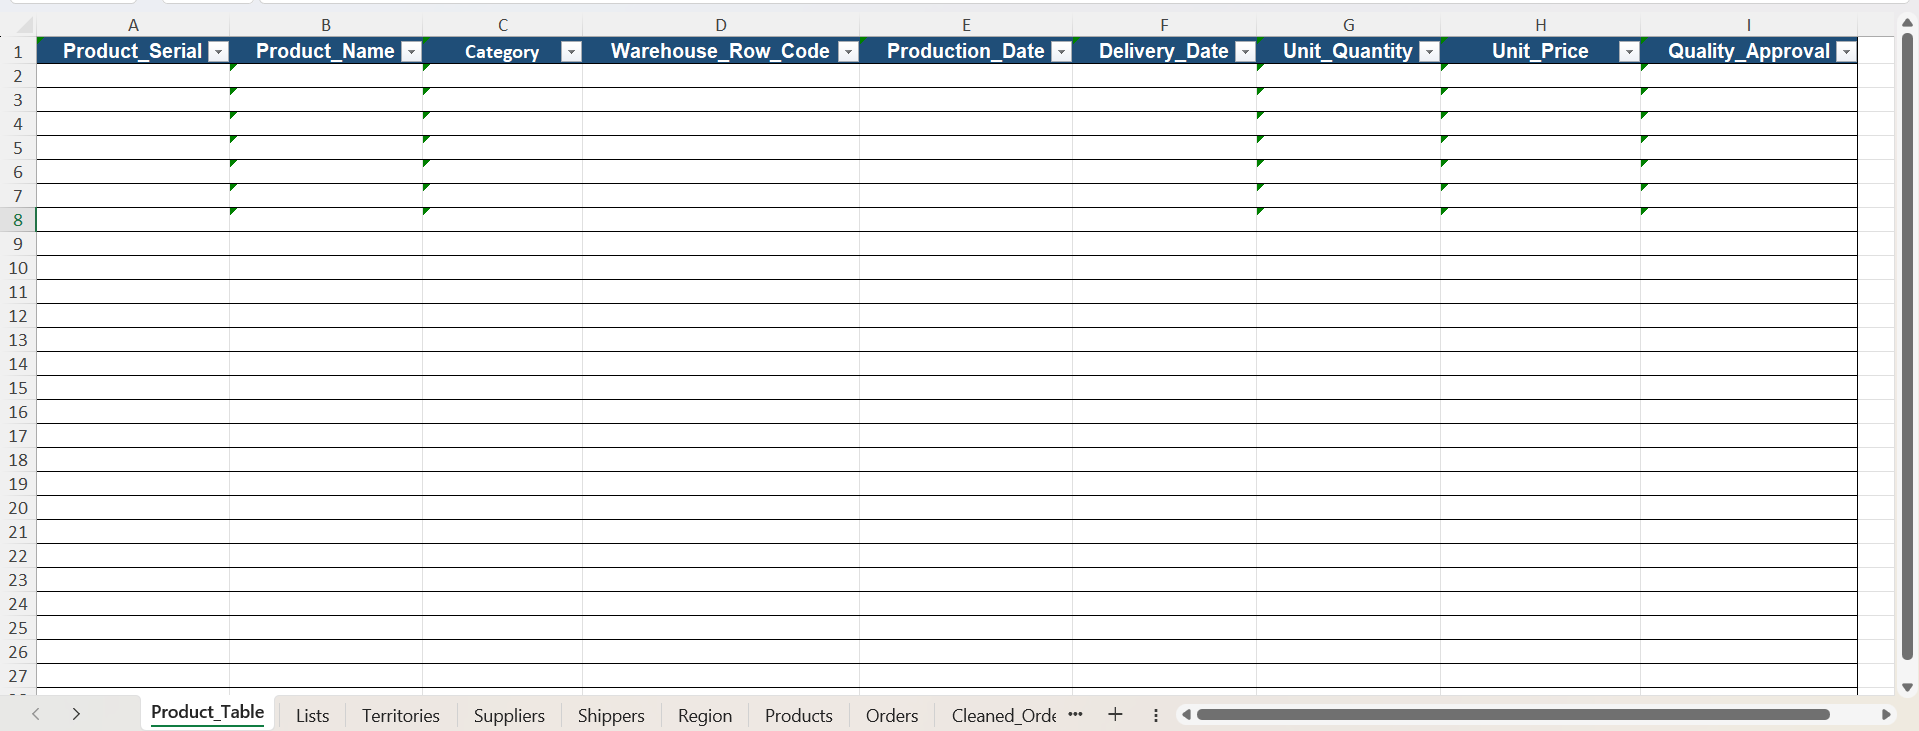
\includegraphics[width=1\textwidth]{phase2_1.png} 
		\caption{تصویر مربوط به طراحی جدول محصولات}
		\label{fig:image1}
	\end{figure}
	
	% -------------------------------------------------------
	\newpage
	\subsection{پاک‌سازی و تبدیل داده‌ها با ابزار کوئری‌سازی}
	
	در ابتدای این بخش، تمامی فایل‌های داده‌ای تمیزشده که در مرحله پیش‌پردازش\LTRfootnote{Preprocessing} تهیه شده بودند، وارد محیط مایکروسافت اکسل شدند. پس از بارگذاری\LTRfootnote{Load} جدول‌ها، نوع داده\LTRfootnote{Data Type} تمامی ستون‌ها مورد بررسی قرار گرفت تا اطمینان حاصل شود هر ستون با نوع داده مناسب خود ذخیره شده است. این مرحله اهمیت زیادی دارد، زیرا تشخیص نادرست نوع داده می‌تواند باعث بروز خطا در محاسبات، مرتب‌سازی، فیلتر کردن\LTRfootnote{Filtering} و تحلیل‌های بعدی شود.
	
	در ادامه، ستون‌هایی که نوع داده آن‌ها به‌درستی تشخیص داده نشده بود اصلاح شدند. برای مثال، ستون‌های تاریخ به قالب تاریخی\LTRfootnote{Date}، ستون‌های عددی به قالب عددی و ستون‌های شناسه یا داده‌های متنی به قالب متنی\LTRfootnote{Text} تبدیل شدند. این استانداردسازی موجب شد تمامی داده‌ها با ساختاری یکنواخت در اختیار مراحل بعدی پردازش قرار گیرند و از بروز ناسازگاری هنگام انجام محاسبات، ایجاد جدول محوری\LTRfootnote{Pivot Table} و استفاده از فرمول‌های اکسل جلوگیری شود.
	
	برای افزایش خوانایی داده‌ها و کاهش تعداد ستون‌های تکراری، بخشی از اطلاعات مرتبط با یکدیگر در قالب ستون‌های جدید ادغام شدند. در جدول مشتریان و تأمین‌کنندگان، اطلاعات شماره تلفن و نمابر\LTRfootnote{Fax} در یک ستون مشترک قرار گرفت تا تمامی اطلاعات تماس در یک محل قابل مشاهده باشند. در مواردی که مقدار نمابر وجود نداشت، عبارت «بدون نمابر» درج شد تا مشخص باشد مقدار خالی ناشی از نبود این اطلاعات است و نه خطای داده‌ای. همچنین اطلاعات مربوط به کشور، شهر و نشانی در قالب یک ستون جدید با عنوان «موقعیت» ترکیب شدند. این کار باعث شد اطلاعات مکانی هر رکورد به صورت یک مقدار کامل و قابل فهم نمایش داده شود و استفاده از آن در گزارش‌ها، فیلترها و تحلیل‌های مکانی ساده‌تر گردد.
	
	\begin{figure}[H]
		\centering
	
	% تصویر سمت راست
		\begin{minipage}{0.48\textwidth}
			\centering
			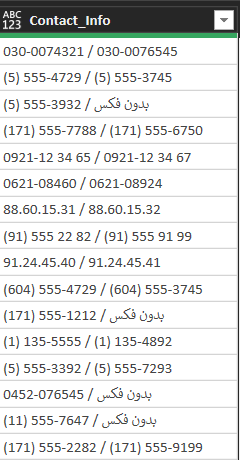
\includegraphics[width=0.9\linewidth,
			height=0.3\textheight,
			keepaspectratio]{phase2_2.png}
			\caption{ادغام تلفن و فکس در یک ستون مشترک }
			\label{fig:image2}
		\end{minipage}
		\hfill % ایجاد فاصله بین دو تصویر
	% تصویر سمت چپ
		\begin{minipage}{0.48\textwidth}
			\centering
			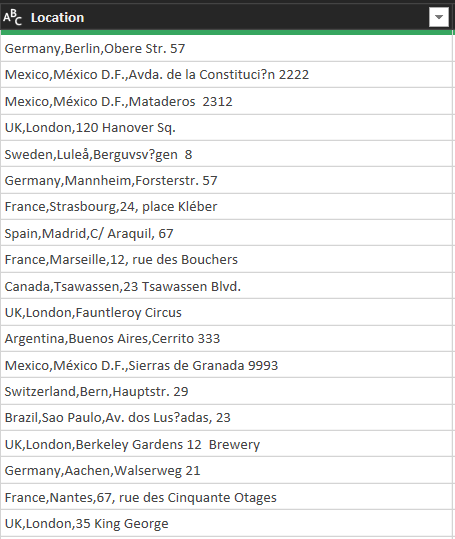
\includegraphics[width=1\linewidth,
			height=0.3\textheight,
			keepaspectratio]{phase2_3.png}
			\caption{داده‌های موقعیت پس از ادغام در یک ستون واحد}
			\label{fig:image3}
		\end{minipage}
	
	\end{figure}
	
	
	پس از استانداردسازی ساختار داده‌ها، قالب نمایش برخی ستون‌ها متناسب با ماهیت اطلاعات آن‌ها اصلاح شد. ستون تخفیف به قالب درصد\LTRfootnote{Percentage} تبدیل شد تا مقدار واقعی تخفیف برای کاربران قابل درک‌تر باشد. همچنین ستون‌های مرتبط با قیمت، مانند قیمت واحد و قیمت کل، با قالب پولی\LTRfootnote{Currency} نمایش داده شدند تا مقادیر مالی با خوانایی بیشتری ارائه شوند.
	
	علاوه بر این، ستون «توقف تولید» که به‌صورت مقادیر عددی صفر و یک\LTRfootnote{Binary Data} ذخیره شده بود، به مقادیر متنی معنادار تبدیل شد؛ به‌طوری‌که مقدار ۰ به «در حال تولید» و مقدار ۱ به «توقف تولید» تغییر یافت. این تبدیل باعث شد بدون نیاز به مراجعه به مستندات، وضعیت هر محصول به‌صورت مستقیم برای کاربران قابل تفسیر باشد.
	
	در همین مرحله، شاخص محبوبیت کالا نیز بر اساس مجموع تعداد فروش و سطح بازسفارش\LTRfootnote{Reorder Level} محاسبه شد و محصولات در چهار گروه \lr{A, B, C, D}   طبقه‌بندی شدند. این دسته‌بندی امکان مقایسه سریع محصولات از نظر میزان تقاضا و اهمیت تجاری آن‌ها را فراهم می‌کند و مبنایی برای تحلیل‌های مدیریتی\LTRfootnote{Management Analysis} محسوب می‌شود.
	
	
	
	\begin{figure}[H]
		\centering
		% به جای picture1.png نام عکس واقعی خود را قرار دهید
		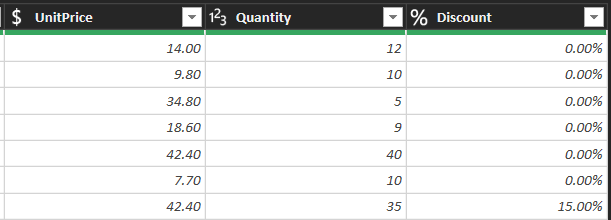
\includegraphics[width=1\textwidth]{phase2_4.png} 
		\caption{قالب‌بندی ستون‌های تخفیف، قیمت واحد و قیمت کل}
		\label{fig:image4}
	\end{figure}
	
	\begin{figure}[H]
		\centering
		% به جای picture1.png نام عکس واقعی خود را قرار دهید
		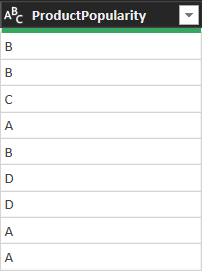
\includegraphics[width=0.5\textwidth,height=0.2\textheight,
		keepaspectratio]{phase2_5.png} 
		\caption{ایجاد ستون شاخص محبوبیت کالا}
		\label{fig:image5}
	\end{figure}
	
	در بخش پایانی، تعدادی ویژگی\LTRfootnote{Feature} جدید از روی داده‌های موجود استخراج شد تا اطلاعات قابل استفاده‌تری برای تحلیل ایجاد شود. هر كالا با استفاده از مقدار موجودي انبار و نقطه سفارش مجدد و کالای سفارش داده تعيين شد و محصولات در وضعیت‌هایی مانند «مطلوب»، «نیازمند سفارش» و «بررسی توقف تولید» قرار گرفتند. سپس با استفاده از قالب‌بندی شرطی\LTRfootnote{Conditional Formatting}، برای هر وضعیت رنگ متفاوتی اختصاص داده شد تا تشخیص شرایط محصولات تنها با مشاهده جدول امکان‌پذیر باشد.
	
	همچنین با استفاده از قیمت واحد، تعداد کالا و میزان تخفیف، هزینه نهایی هر سفارش محاسبه و در قالب ستون «قیمت کل» ثبت شد. این ویژگی بدون نیاز به انجام محاسبات مجدد، امکان بررسی ارزش مالی سفارش‌ها و تحلیل‌های مرتبط با فروش را فراهم می‌کند و می‌تواند در تهیه گزارش‌های مدیریتی مورد استفاده قرار گیرد. این فرآیند استخراج ویژگی\LTRfootnote{Feature Extraction}، گام نهایی برای تبدیل داده‌های خام به اطلاعات ارزشمند جهت تصمیم‌گیری بود.
	
	\begin{figure}[H]
		\centering
		
		% تصویر سمت راست
		\begin{minipage}{0.4\textwidth}
			\centering
			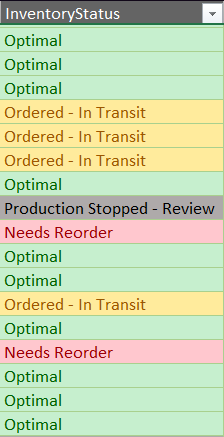
\includegraphics[width=\textwidth]{phase2_6.png}
			\caption{تقسیم وضعیت کالا به 4 حالت: مطلوب، درحال ارسال، نیازمند سفارش، توقف تولید}
			\label{fig:image6}
		\end{minipage}
		\hfill % ایجاد فاصله بین دو تصویر
		% تصویر سمت چپ
		\begin{minipage}{0.4\textwidth}
			\centering
			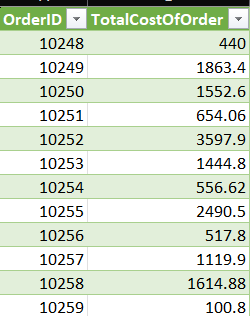
\includegraphics[width=\textwidth]{phase2_7.png}
			\caption{محاسبه ارزش سفارش ها}
			\label{fig:image7}
		\end{minipage}
		
	\end{figure}
	
	% -------------------------------------------------------
	\newpage
	\subsection{مدل‌سازی و تحلیل داده‌ها}
	
	در بخش مدل‌سازی و تحلیل داده‌ها، ابتدا تمامی جداول پایگاه داده وارد محیط مدل داده\LTRfootnote{Data Model} اکسل شدند. در این مرحله، ارتباطات منطقی میان جداول (از جمله جداول سفارشات، محصولات، تأمین‌کنندگان، شرکت‌های حمل‌ونقل و دسته‌بندی‌ها) بر اساس کلیدهای اصلی و کلیدهای خارجی به‌طور کامل برقرار گردید. برقرار ساختن این ارتباطات\LTRfootnote{Relationships} به سیستم اجازه می‌دهد تا داده‌ها را از جداول مختلف به‌صورت یکپارچه فراخوانی و تحلیل کند.
	
	پس از حصول اطمینان از یکپارچگی روابط، پنج تحلیل کلیدی با بهره‌گیری از ابزارهای جدول محوری و نمودار محوری\LTRfootnote{PivotChart} به‌منظور استخراج بینش‌های تجاری طراحی و پیاده‌سازی شد. 
	\subsubsection{ﻧﻤﺎﻳﺶ ﻣﻘﺪﺍﺭ ﺳﻔﺎﺭﺵ ﺟﺪﻳﺪ ﺑﺮﺍﻱ ﻫﺮ ﺩﺳﺘﻪ ﺑﻨﺪﻱ ﺩﺭ ﺟﺪﻭﻝ ﻣﺤﻮﺭﻱ}
	در تحلیل نخست، با هدف پایش وضعیت تأمین کالا، مجموع مقدار سفارشات در راه\LTRfootnote{UnitsOnOrder} به تفکیک هر نام دسته‌بندی\LTRfootnote{CategoryName} استخراج شد. این تحلیل به مدیران کمک می‌کند تا دید دقیقی نسبت به حجم کالاهای در حال ورود به انبار برای هر گروه کالایی داشته باشند.
	
		\begin{figure}[H]
		\centering
		% به جای picture1.png نام عکس واقعی خود را قرار دهید
		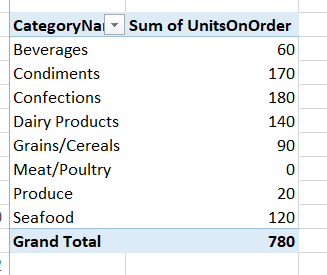
\includegraphics[width=0.6\textwidth]{phase2_8.png} 
		\caption{ تحلیل اول: ﻧﻤﺎﻳﺶ ﻣﻘﺪﺍﺭ ﺳﻔﺎﺭﺵ ﺟﺪﻳﺪ ﺑﺮﺍﻱ ﻫﺮ ﺩﺳﺘﻪ ﺑﻨﺪﻱ}
		\label{fig:analysis1}
	\end{figure}
	\subsubsection{ﺗﺤﻠﻴﻞ ﻫﺰﻳﻨﻪ ﺣﻤﻞ ﺑﻪ ﺗﻔﻜﻴﻚ ﻛﺸﻮﺭ ﻭ ﺷﺮﻛﺖ ﺣﻤﻞ ﻭ ﻧﻘﻞ ﻫﻤﺮﺍﻩ ﺑﺎ ﻧﻤﻮﺩﺍﺭ}
	در تحلیل دوم، به منظور ارزیابی دقیق هزینه‌های لجستیک، شاخص هزینه حمل‌ونقل بر اساس تقاطع دو بعد «کشور مقصد»\LTRfootnote{ShipCountry} و «شرکت حمل‌ونقل»\LTRfootnote{Shippers} مورد بررسی قرار گرفت و خروجی آن به صورت یک نمودار ستونی خوشه‌ای ارائه گردید.
	
	\begin{figure}[H]
		\centering
		% به جای picture2.png نام عکس واقعی خود را قرار دهید
		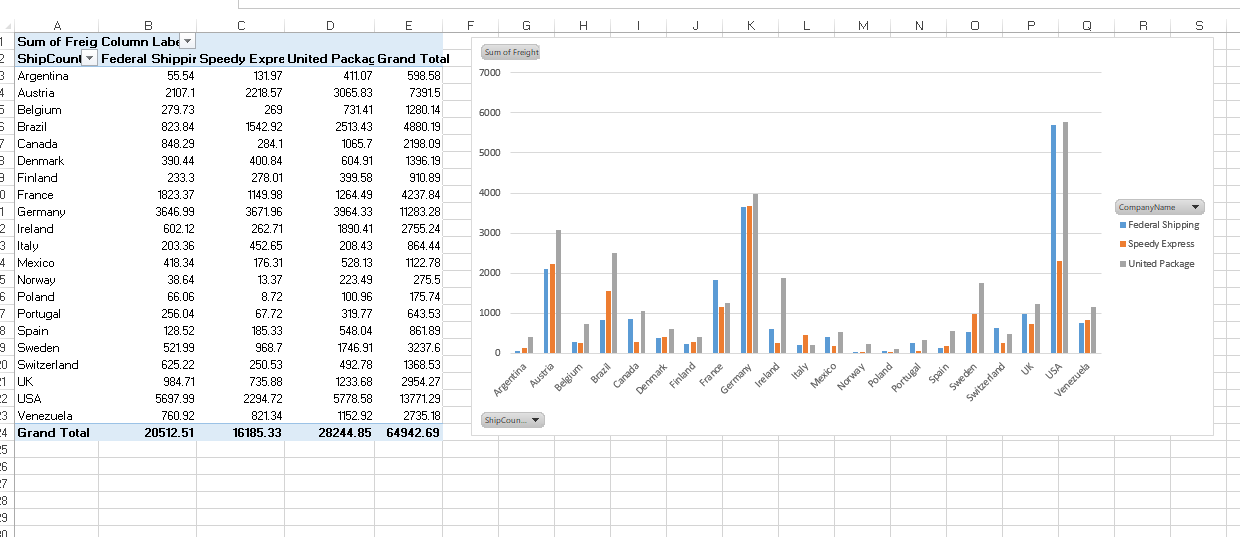
\includegraphics[width=1\textwidth]{phase2_9.png}
		\caption{تحلیل دوم: توزیع هزینه‌های لجستیک و حمل‌ونقل بر اساس کشور مقصد و شرکت باربری}
		\label{fig:analysis2}
	\end{figure}
	\subsubsection{ ﺗﺤﻠﻴﻞ ﺗﻘﺎﺿﺎ ﻭ ﻗﻴﻤﺖ ﻭﺍﺣﺪ ﻛﺎﻻ ﻭ ﻧﻤﺎﻳﺶ ﺑﺼﺮﻱ ﻣﻘﺪﺍﺭ ﻓﺮﻭﺵ ﻫﺮ ﻛﺎﻻ}
	برای تحلیل سوم، رفتار بازار در قبال قیمت‌گذاری محصولات ارزیابی شد؛ به این صورت که «مقدار کل تقاضا»\LTRfootnote{Total Quantity Sold} در مقابل «میانگین قیمت واحد»\LTRfootnote{Average Unit Price} هر محصول قرار گرفت و این نتایج در قالب نمودار ترکیبی\LTRfootnote{Combo Chart} با استفاده از محور ثانویه\LTRfootnote{Secondary Axis} نمایش داده شد تا همبستگی میان قیمت و حجم فروش به‌وضوح قابل درک باشد.
	
	\begin{figure}[H]
		\centering
	
	% به جای picture3.png نام عکس واقعی خود را قرار دهید
	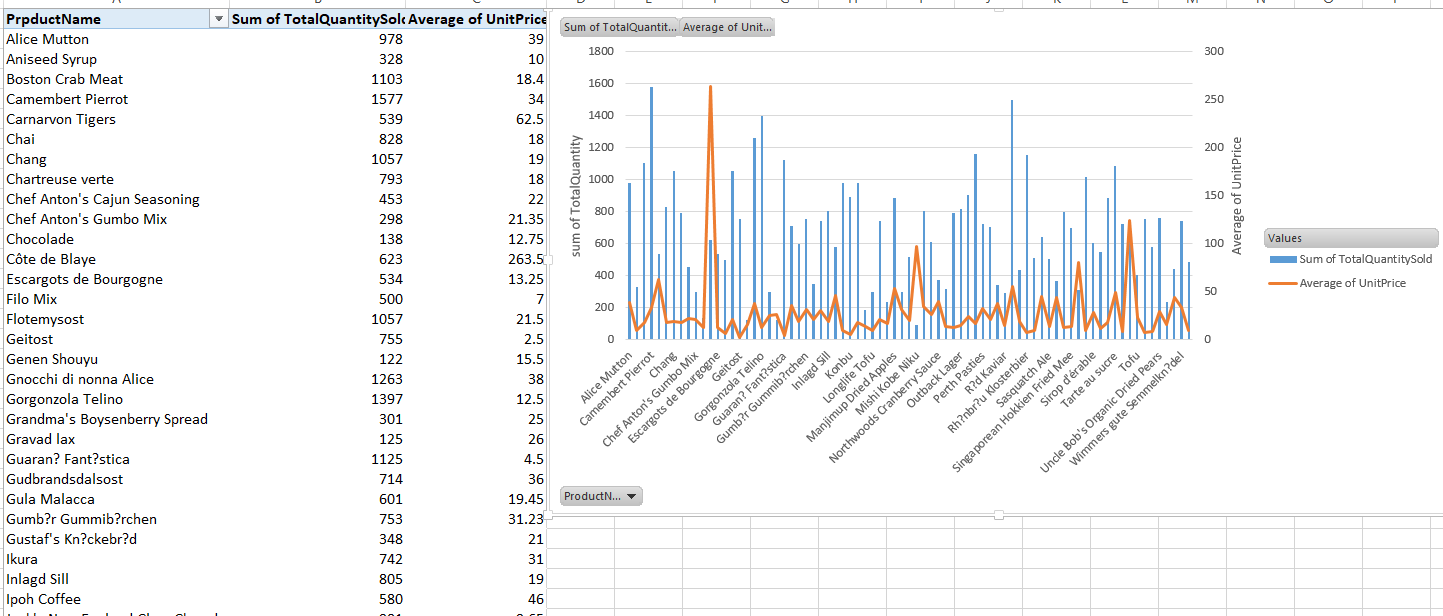
\includegraphics[width=1\textwidth,height=0.2\textheight]{phase2_10.png}
		\caption{تحلیل سوم: همبستگی میانگین قیمت واحد و میزان تقاضا (نمودار ترکیبی)}
		\label{fig:analysis3}
	\end{figure}
	\subsubsection{ﺗﺤﻠﻴﻞ ﺍﺭﺯﺵ ﻛﻞ ﻣﻮﺟﻮﺩﻱ ﺍﻧﺒﺎﺭ ﺑﻪ ﺗﻔﻜﻴﻚ ﺗﺄﻣﻴﻦ ﻛﻨﻨﺪﮔﺎﻥ}
	در ادامه و برای تحلیل چهارم، به منظور برآورد ارزش سرمایه در گردشِ موجود در انبار، ابتدا یک ستون محاسباتی\LTRfootnote{CalculatedColumn} اختصاصی با فرمول ضرب موجودی در قیمت واحد 
	\begin{latin}
	\texttt{UnitInStock*UnitPrice}
	\end{latin}
در جدول محصولات ایجاد گردید. سپس ارزش کل موجودی انبار به تفکیک شرکت‌های تأمین‌کننده محاسبه و در یک نمودار میله‌ای تجمیع شد. 
	
	\begin{figure}[H]
		\centering
		% به جای picture4.png نام عکس واقعی خود را قرار دهید
		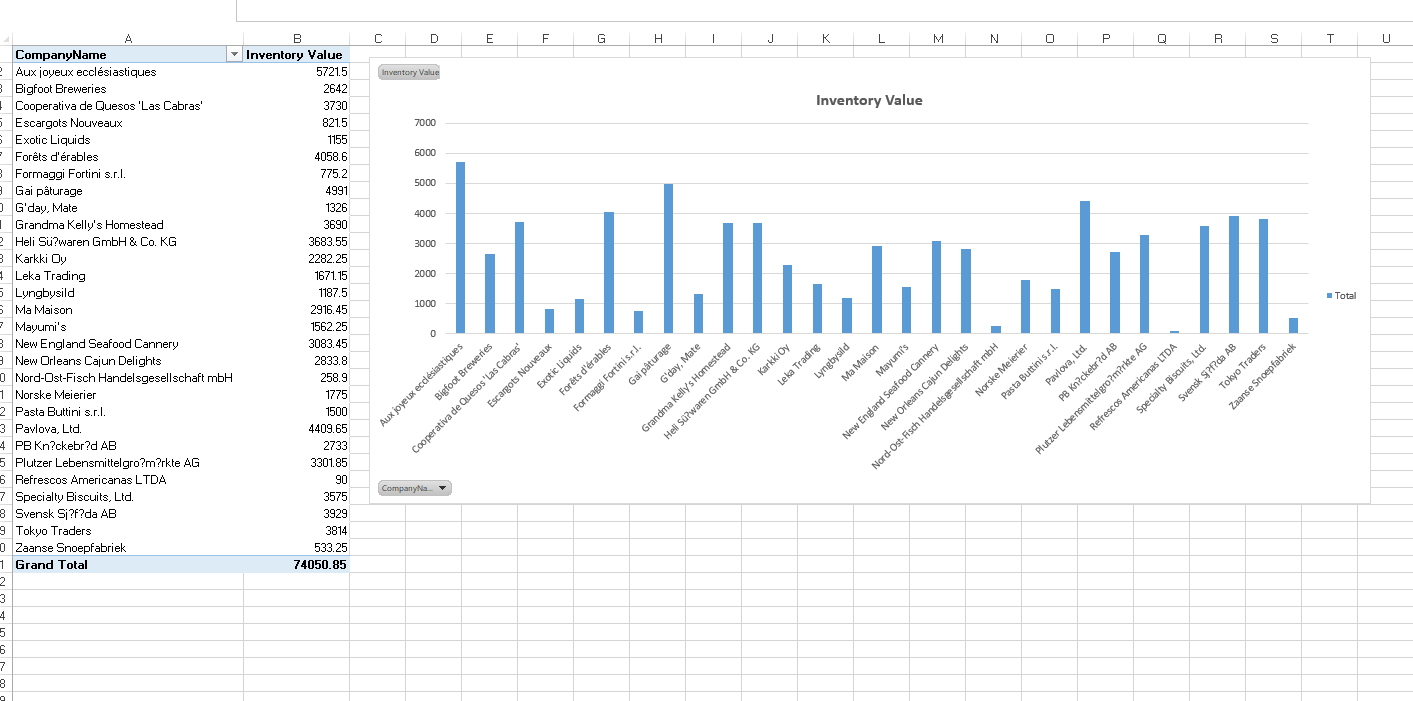
\includegraphics[width=1\textwidth]{phase2_11.png}
		\caption{تحلیل چهارم: برآورد ارزش سرمایه در گردش انبار به تفکیک تأمین‌کنندگان}
		\label{fig:analysis4}
	\end{figure}
	\subsubsection{ﺗﺤﻠﻴﻞ ﺩﺭﺁﻣﺪ ﻛﻞ ﺷﺮﻛﺖ ﺑﻪ ﺗﻔﻜﻴﻚ ﻛﺸﻮﺭ ﻣﻘﺼﺪ ﺑﺎ ﺍﺳﺘﻔﺎﺩﻩ ﺍﺯ ﺑﺮﺵ ﮔﺮ ﻭ ﻧﻤﻮﺩﺍﺭ}
	در تحلیل پنجم که به بررسی درآمد کل شرکت اختصاص داشت، ابتدا به منظور تضمین یکپارچگی داده‌ها، ارتباط استانداردی میان جدول جزئیات پاکسازی‌شده سفارش‌ها\LTRfootnote{CleanOrderDetails} و جدول سفارش‌ها از طریق شناسه سفارش\LTRfootnote{OrderID} برقرار گردید. پس از اتصال این جداول، مجموع هزینه سفارش‌ها\LTRfootnote{TotalCostOfOrder} به عنوان شاخص درآمد کل، به تفکیک کشورهای مقصد محاسبه و مصورسازی شد.
	
	به منظور ارتقای سطح کارایی و تعاملی کردن این گزارش پایانی، ابزار فیلتر گرافیکی یا برش‌دهنده بر روی فیلد تاریخ سفارش\LTRfootnote{OrderDate} پیاده‌سازی گردید. این ویژگی کاربردی به مدیران سازمان امکان می‌دهد تا روند درآمدهای جغرافیایی را به صورت پویا در بازه‌های زمانی مختلف پایش کرده و تصمیم‌گیری‌های کلان مدیریتی را با سرعت و دقت بیشتری انجام دهند.
	
	\begin{figure}[H]
		\centering
		% به جای picture5.png نام عکس واقعی خود را قرار دهید
		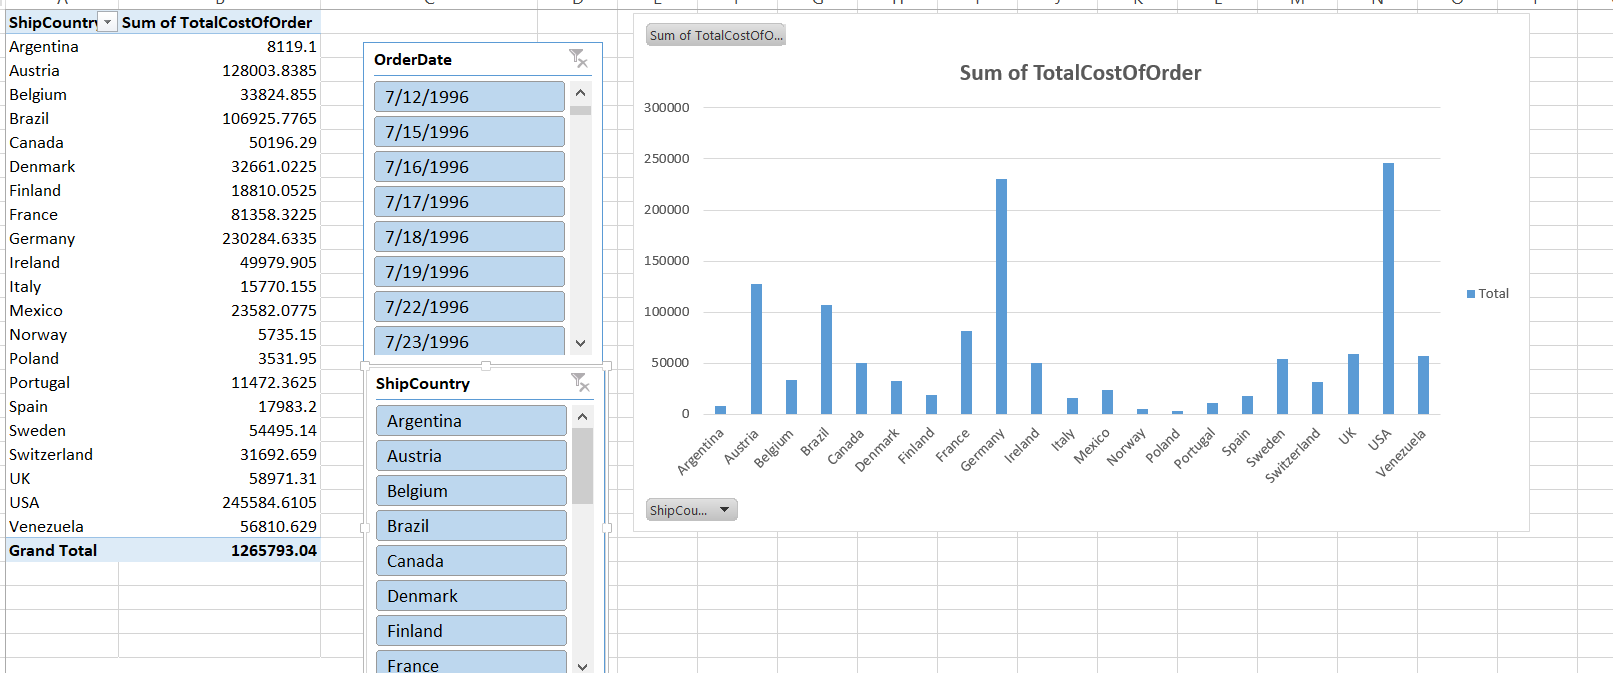
\includegraphics[width=1\textwidth]{phase2_13.png}
		\caption{تحلیل پنجم: درآمد جغرافیایی کل شرکت همراه با فیلتر پویای تاریخ سفارش}
		\label{fig:analysis5}
	\end{figure}
	
	% -------------------------------------------------------
	\subsection{خودکارسازی با ماکرو و برنامه‌نویسی}
	
	در بخش پایانی پروژه و با هدف خودکارسازی\LTRfootnote{Automation} عملیات انبارداری، ارتقای دقت در مدیریت اطلاعات کالاها و به حداقل رساندن خطای انسانی، فرآیند پردازش داده‌ها از طریق توسعه یک ماکرو\LTRfootnote{Macro} در محیط برنامه‌نویسی ویژوال بیسیک برای اپلیکیشن‌ها\LTRfootnote{VBA (Visual Basic for Applications)} پیاده‌سازی شد. این برنامه که در قالب زیرروال \lr{Process WarehouseData} توسعه یافته است، فرآیندهای محاسباتی، قالب‌بندی شرطی و تفکیک داده‌ها را به صورت پویا و در قالب مراحل پیوسته مدیریت می‌کند.
	
	در وهله نخست، سیستم با شناسایی خودکار آخرین ردیف فعال جدول بر اساس ستون تعداد کالا، یک حلقه تکرار\LTRfootnote{Loop} را بر روی تمامی ردیف‌ها آغاز می‌کند. در طول این پیمایش، مقادیر مربوط به تعداد کالا و قیمت واحد پس از اعتبارسنجی عددی و اطمینان از خالی نبودن سلول‌ها، در یکدیگر ضرب شده و به صورت متوالی در متغیر ارزش کل  \LTRfootnote{totalValueSum}        انباشته می‌شوند. در نهایت، حاصل این محاسبات به همراه عنوانِ مشخص در سلول‌های هدف درج شده و برای جلب توجه کاربر، با رنگ زرد متمایز می‌گردد. 
	
	هم‌زمان با این محاسبات، برنامه وضعیت کنترل کیفیت کالاها را در ستون مربوطه ارزیابی می‌کند تا قالب‌بندی ظاهری جدول را به صورت پویا تغییر دهد. بر اساس منطق شرطی تعریف‌شده، ردیف‌هایی که وضعیت آن‌ها تاییدشده\LTRfootnote{Approved} باشد با رنگ سبز ملایم و موارد ردشده\LTRfootnote{Rejected} با رنگ قرمز ملایم متمایز می‌شوند. این در حالی است که ردیف‌های در حال انتظار\LTRfootnote{Pending} بدون تغییر رنگ و با قالب پیش‌فرض باقی می‌مانند تا ساختار بصری جدول به راحتی وضعیت هر کالا را به نمایش بگذارد.
	
	در نهایت، فرآیند استخراج داده‌ها به منظور آرشیو اقلام مجاز و انتقال آن‌ها به یک کاربرگ جدید انجام می‌گیرد. بدین منظور، برنامه ابتدا وجود کاربرگ مجزایی به نام موارد پذیرفته شده\LTRfootnote{Approved\_Items} را بررسی می‌کند؛ در صورت عدم وجود، این کاربرگ ایجاد و ردیف عناوین\LTRfootnote{Header} به آن منتقل می‌شود و در صورت وجود، داده‌های قبلی آن پاکسازی می‌گردند تا اطلاعات جدید جایگزین شوند. در طول پیمایش حلقه، هر ردیفی که وضعیت تاییدشده داشته باشد، به طور خودکار به این کاربرگ جدید کپی می‌شود. 
	
	
	پس از اتمام موفقیت‌آمیز تمامی این مراحل، یک جعبه پیام\LTRfootnote{MessageBox} برای اطلاع‌رسانی به کاربر نمایش داده شده و کل پروژه در فایلی با پسوند پشتیبانی‌کننده از ماکرو در اکسل\LTRfootnote{xlsm} ذخیره می‌گردد تا پایداری و قابلیت اجرای مجدد این فرآیند خودکار تضمین شود.
	\begin{figure}[H]
		\centering
		% به جای picture5.png نام عکس واقعی خود را قرار دهید
		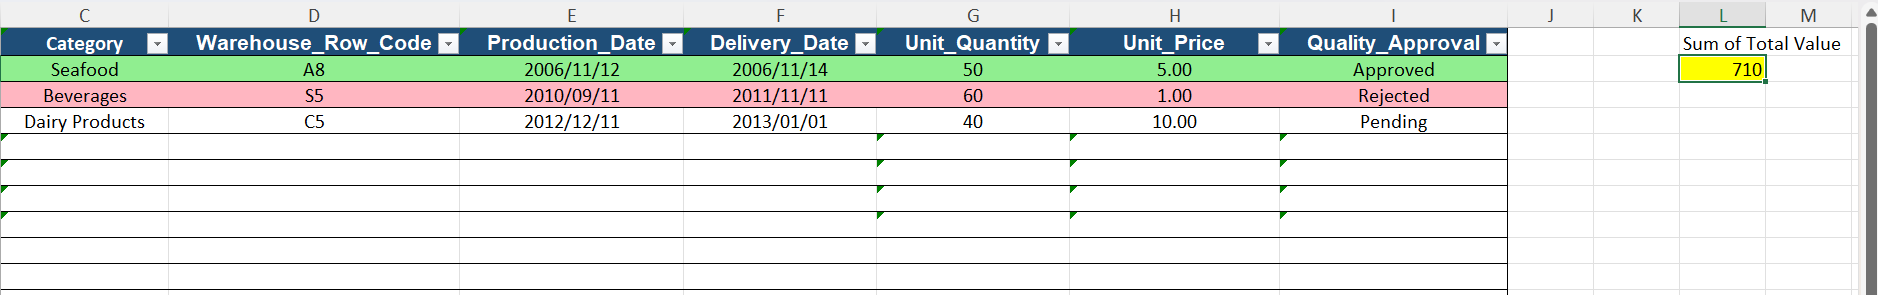
\includegraphics[width=1\textwidth]{phase2_14.png}
		\caption{نمونه‌ای از نحوه عملکرد کد }
		\label{fig:image14}
	\end{figure}
	\begin{figure}[H]
		\centering
		% به جای picture5.png نام عکس واقعی خود را قرار دهید
		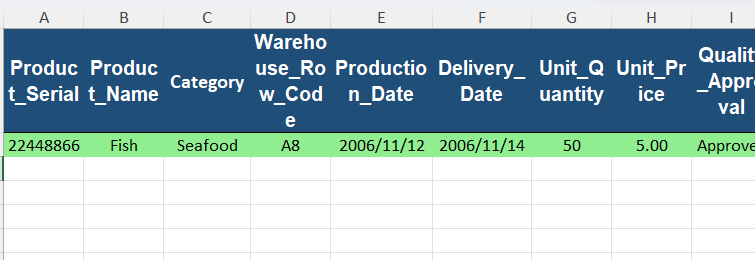
\includegraphics[width=1\textwidth]{phase2_15.png}
		\caption{کاربرگ جدید ساخته‎‌شده برای کالاهای پذیرفته‌شده  }
		\label{fig:omage15}
	\end{figure}
	
	
	
	% --- بخش چهارم (فاز سوم) ---
	\newpage
	\section{فاز سوم}
	
	\subsection{طراحی جداول و روابط}
	در این مرحله از پروژه، پیاده‌سازی پایگاه داده تراکنشی\LTRfootnote{Transactional Database} شرکت نورث‌ویند در محیط نرم‌افزار مایکروسافت اکسس\LTRfootnote{Microsoft Access} با هدف ایجاد یک سیستم یکپارچه برای مدیریت چرخه فروش و تأمین آغاز گردید. فرآیند طراحی با تحلیل دقیق فایل‌های منبع و آماده‌سازی آن‌ها جهت انتقال به بانک اطلاعاتی صورت پذیرفت. پیش از هرگونه اقدام، تمامی فایل‌های سی اس وی به‌منظور درک دقیق ساختار فیلدها و تعیین نوع داده‌ها، در محیط دفترچه یادداشت ویندوز \LTRfootnote{Notepad} بررسی شدند. این پیش‌بینی فنی سبب شد تا در هنگام استفاده از جادوگر واردسازی متن\LTRfootnote{Import Text Wizard}، تنظیمات مربوط به جداکننده\LTRfootnote{Delimiter} بر روی کاما و مشخص‌کننده متن\LTRfootnote{Text Qualifier} بر روی نقل‌قول دوتایی\LTRfootnote{Double Quote} تنظیم گردد؛ این امر از شکستگی داده‌های متنی که حاوی کاراکتر کاما بودند جلوگیری کرده و سلامت اطلاعات را در هنگام ورود تضمین نمود.
	
	بمنظور ارتقای دقت در مدیریت زمان و تاریخ، از بخش تنظیمات پیشرفته واردسازی\LTRfootnote{Advanced Import Specifications} استفاده شد. با تنظیم کدگذاری بر روی یونیکد\LTRfootnote{UTF-8} و انتخاب قالب تاریخ\LTRfootnote{YMD} (سال-ماه-روز) و فعال کردن تیک \lr{leading zeros in dates} تاریخ سفارش\LTRfootnote{OrderDate} و تاریخ استخدام\LTRfootnote{HireDate} بدون بروز خطای تبدیل، به نوع داده استاندارد تاریخ و زمان\LTRfootnote{Date/Time} مجهز شدند. پس از استقرار داده‌ها در جداول، ساختار کلیدهای اصلی برای تمامی جداول پایه تعریف گردید تا یکتایی هر رکورد تضمین شود. در این میان، برای جداول واسط\LTRfootnote{Junction Tables} همچون جزئیات سفارش\LTRfootnote{Order Details} و قلمرو کارکنان\LTRfootnote{EmployeeTerritories}، از کلید اصلی مرکب استفاده شد تا منطق روابط چند‌به‌چند\LTRfootnote{Many-to-Many} به درستی پیاده‌سازی شده و از ثبت رکوردهای تکراری در یک تراکنش واحد جلوگیری شود.
	
	در گام نهایی، معماری ارتباطی پایگاه داده در بخش روابط شکل گرفت. با تعریف کلیدهای خارجی، مجموعاً ۱۰ رابطه منطقی از نوع یک‌به‌چند\LTRfootnote{One-to-Many} میان موجودیت‌های سیستم برقرار شد. نکته حائز اهمیت در این بخش، فعال‌سازی گزینه اجبار یکپارچگی ارجاعی\LTRfootnote{Enforce Referential Integrity} در تمامی روابط بود. این محدودیت سیستمی با جلوگیری از ایجاد رکوردهای یتیم\LTRfootnote{Orphan Records} و اطمینان از وجود کلیدهای مرجع پیش از ثبت داده‌های وابسته، پایداری و صحت منطقی پایگاه داده را برای مراحل بعدی یعنی طراحی پرس‌وجوها و گزارش‌های مدیریتی تضمین نمود.
	
	\begin{figure}[H]
		\centering
		% به جای picture5.png نام عکس واقعی خود را قرار دهید
		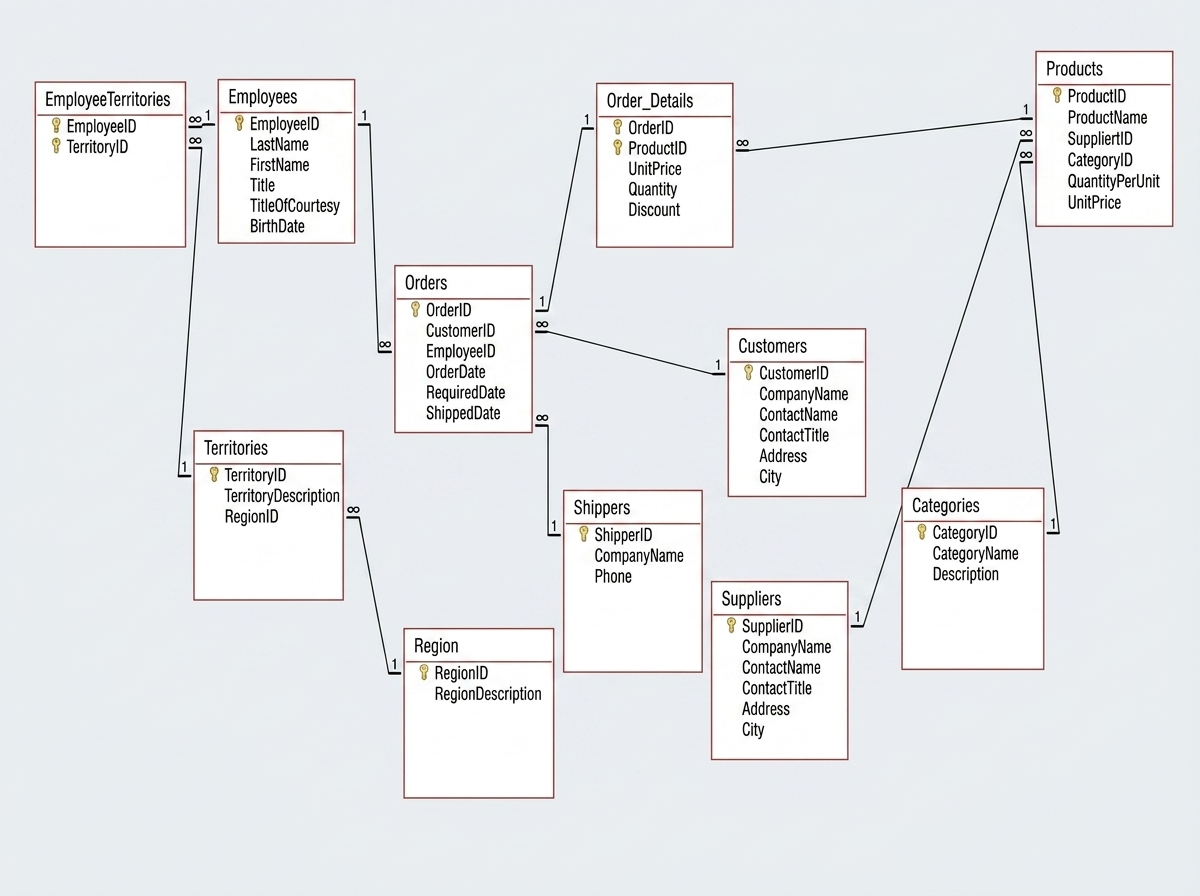
\includegraphics[width=1\textwidth]{phase3_1.png}
		\caption{نمودار روابط جداول در پایگاه داده }
		\label{fig:phase3_1}
	\end{figure}
	
	
	
	\subsection{طراحی کوئری‌ها}
	\subsubsection{نشان دادن ﻧﺎﻡ ﻣﺤﺼﻮﻝ ﻭ ﻗﻴﻤﺖ ﻧﻬﺎﻳﻲ ﺁﻥ ﭘﺲ ﺍﺯ ﺍﻋﻤﺎﻝ ﺗﺨﻔﻴﻒ }
	پس از تثبیت ساختار جداول و برقراری روابط منطقی میان موجودیت‌ها، فرآیند پیاده‌سازی پرس‌وجوها\LTRfootnote{Queries} به منظور پاسخگویی به نیازهای تحلیلی کسب‌وکار و استخراج اطلاعات ارزش‌آفرین آغاز گردید. در وهله نخست، هدف سیستم بر محاسبه قیمت نهایی محصولات پس از اعمال تخفیف‌های تجاری متمرکز شد. برای پیاده‌سازی این سناریو، پرس‌وجوی محاسباتی ویژه‌ای طراحی گردید که در آن با استفاده از فرمول‌نویسی در یک ستون محاسباتی، مقدار نهایی با کسر ۲۰ درصد تخفیف تعیین شد. در این فرمول که به صورت:
	\vspace{0.2cm}
	\begin{latin}
		\texttt{FinalPrice: Round([UnitPrice] * 0.8)}
	\end{latin}
	\vspace{0.3cm}
	تعریف گردید، از تابع گرد کردن\LTRfootnote{Round} استفاده شد تا خروجی نهایی به نزدیک‌ترین عدد صحیح تبدیل شود؛ این رویکرد محاسباتی علاوه بر ساده‌سازی فرآیندهای مالی، انطباق کاملی با استانداردهای سیستم‌های حسابداری و صدور فاکتور دارد.

	
	\begin{figure}[H]
		\centering
		
		% تصویر سمت راست
		\begin{minipage}{0.48\textwidth}
			\centering
			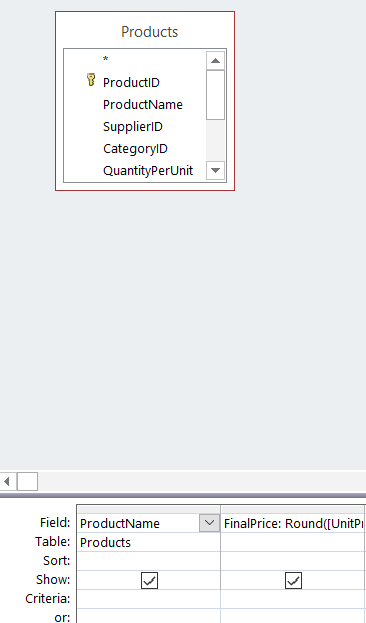
\includegraphics[width=1\linewidth,
			height=0.25\textheight]{phase3_2.png}
			\caption{ﻛﻮﺋﺮﻱ ﻧﺎﻡ ﻣﺤﺼﻮﻝ ﻭ ﻗﻴﻤﺖ ﻧﻬﺎﻳﻲ ﺁﻥ ﭘﺲ ﺍﺯ ﺍﻋﻤﺎﻝ ﺗﺨﻔﻴﻒ}
			\label{fig:hase3_2}
		\end{minipage}
		\hfill % ایجاد فاصله بین دو تصویر
		% تصویر سمت چپ
		\begin{minipage}{0.48\textwidth}
			\centering
			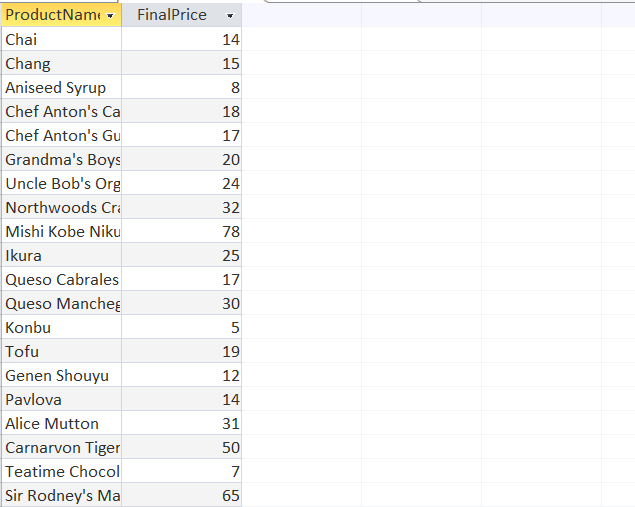
\includegraphics[width=1\linewidth,
			height=0.25\textheight]{phase3_d.png}
			\caption{نتیجه کوئری}
			\label{fig:[hase3_s]}
		\end{minipage}
		
	\end{figure}
	
	\subsubsection{نشان دادن ﻧﺎﻡ ﻫﺮ ﻣﺤﺼﻮﻝ ﺑﻪ ﻫﻤﺮﺍﻩ ﺗﻌﺪﺍﺩ ﻛﻞ ﺳﻔﺎﺭﺵ ها}
	در گام بعدی و به منظور بررسی رفتار بازار، پرس‌وجوی تحلیل محبوبیت و میزان تقاضای محصولات طراحی و اجرا شد. این ساختار تحلیلی با ادغام\LTRfootnote{Join} جدول کالاها و جزئیات سفارش‌ها بر اساس فیلد مشترک شناسه کالا\LTRfootnote{ProductID} شکل گرفت. سیستم با بهره‌گیری از توابع تجمعی\LTRfootnote{Aggregate Functions}، کالاها را بر اساس نام تجاری آن‌ها گروه‌بندی\LTRfootnote{Group By} نموده و تعداد دفعات ثبت هر کالا در فاکتورهای مختلف را با استفاده از تابع شمارش\LTRfootnote{Count} بر روی فیلد شناسه سفارش\LTRfootnote{OrderID} محاسبه کرد. خروجی حاصل از این تحلیل، مدیران زنجیره تأمین را قادر می‌سازد تا اقلام پرتقاضا را شناسایی کرده و تصمیمات دقیق‌تری در خصوص کنترل موجودی انبار اتخاذ نمایند.

	
	\begin{figure}[H]
		\centering
		
		% تصویر سمت راست
		\begin{minipage}{0.48\textwidth}
			\centering
			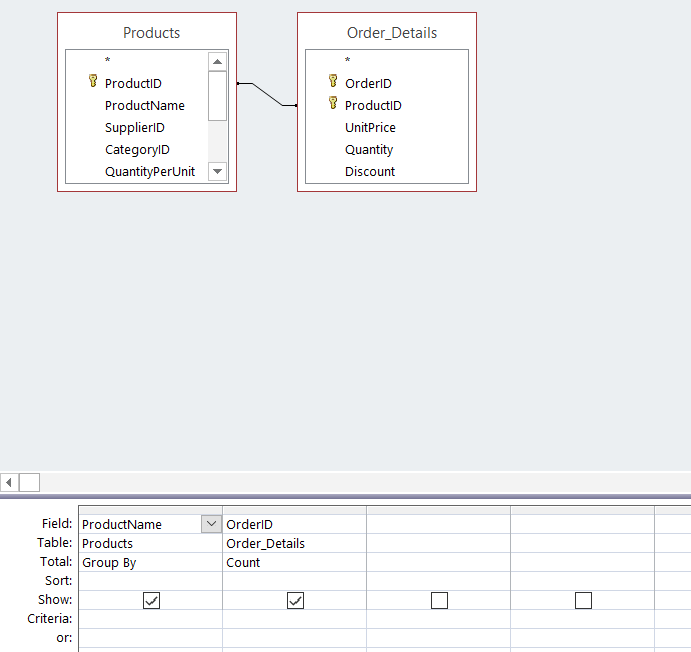
\includegraphics[width=1\linewidth,
			height=0.2\textheight]{phase3_3.png}
			\caption{ﻛﻮﺋﺮﻱ ﻧﺎﻡ ﻫﺮ ﻣﺤﺼﻮﻝ ﺑﻪ ﻫﻤﺮﺍﻩ ﺗﻌﺪﺍﺩ ﻛﻞ ﺳﻔﺎﺭﺵ ﻫﺎﻱ ﺛﺒﺖ ﺷﺪﻩ}
			\label{fig:hase3_3}
		\end{minipage}
		\hfill % ایجاد فاصله بین دو تصویر
		% تصویر سمت چپ
		\begin{minipage}{0.48\textwidth}
			\centering
			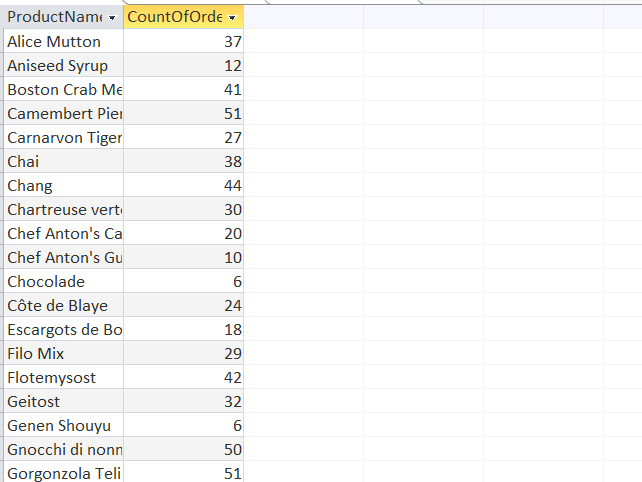
\includegraphics[width=1\linewidth,
			height=0.2\textheight]{phase3_qd.png}
			\caption{نتیجه کوئری}
			\label{fig:phase3_s]}
		\end{minipage}
		
	\end{figure}
	
	\subsubsection{نشان دادن   ﻧﺎﻡ ﻫﺮ ﻛﺎﺭﻣﻨﺪ ﺑﻪ ﻫﻤﺮﺍﻩ ﺗﻌﺪﺍﺩ ﻛﻞ ﺳﻔﺎﺭﺵ ها توسط او}
	در نهایت، بخش ارزیابی عملکرد و بهره‌وری منابع انسانی با طراحی پرس‌وجوی سوم پیاده‌سازی گردید. هدف از این بخش، سنجش کارایی کارکنان بخش فروش بر اساس حجم تراکنش‌های ثبت‌شده توسط آنان بود. بدین منظور، با برقراری پیوند میان جدول کارکنان و جدول سفارش‌ها از طریق شناسه کارمند\LTRfootnote{EmployeeID}، اطلاعات این دو بخش یکپارچه گردید. در این ساختار، سیستم پس از گروه‌بندی سوابق بر اساس نام خانوادگی کارکنان، تعداد کل سفارش‌های ثبت‌شده توسط هر فرد را از طریق اعمال تابع شمارش بر روی فیلد شناسه سفارش استخراج نمود. خروجی این پرس‌وجو به عنوان یک شاخص کلیدی عملکرد در ارزیابی‌های دوره‌ای سازمان و تخصیص پاداش‌های فروش نقش مؤثری ایفا می‌کند.
	
	\begin{figure}[H]
		\centering
		
		% تصویر سمت راست
		\begin{minipage}{0.48\textwidth}
			\centering
			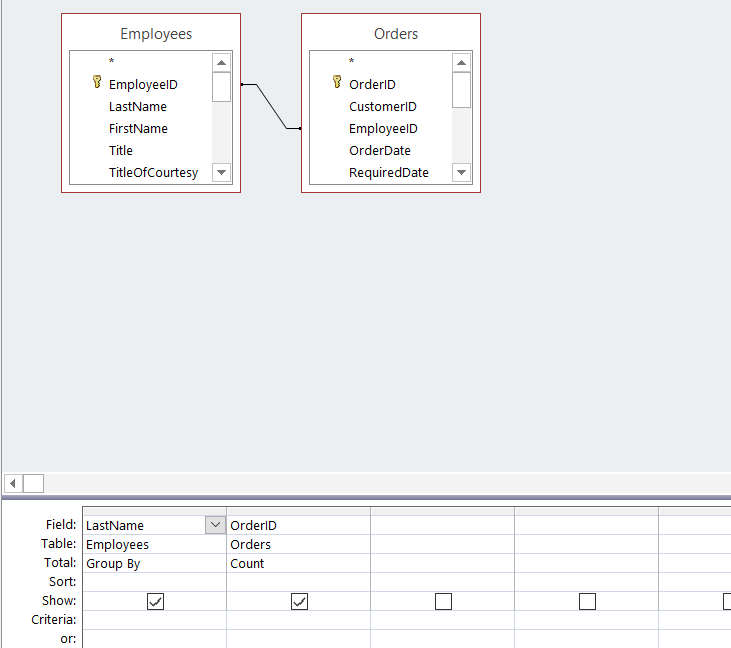
\includegraphics[width=1\linewidth,
			height=0.3\textheight]{phase3_4.png}
			\caption{نتیجه ﻛﻮﺋﺮﻱ}
			\label{fig:hase3_e}
		\end{minipage}
		\hfill % ایجاد فاصله بین دو تصویر
		% تصویر سمت چپ
		\begin{minipage}{0.48\textwidth}
			\centering
			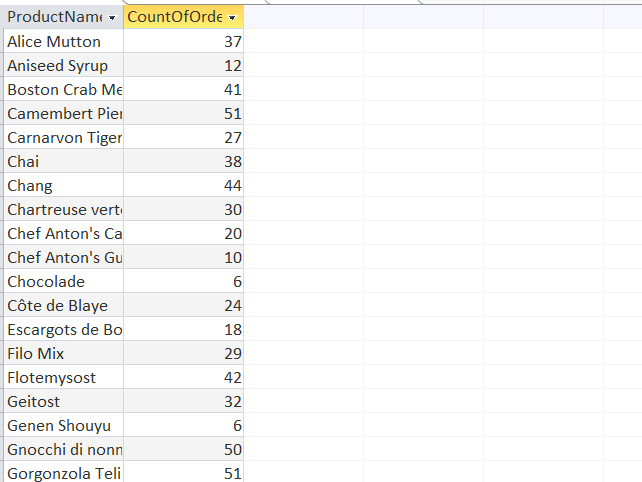
\includegraphics[width=1\linewidth,
			height=0.2\textheight]{phase3_qd.png}
			\caption{نتیجه کوئری}
			\label{fig:phase3_sa}
		\end{minipage}
		
	\end{figure}
	
	
	\subsection{طراحی فرم‌های پایگاه داده}
	یکی از اصول بنیادین در توسعه سیستم‌های مدیریت پایگاه داده\LTRfootnote{Database Management System}، جداسازی کامل لایه کاربر\LTRfootnote{User Interface} از لایه داده\LTRfootnote{Data Layer} به منظور تسهیل تعامل کاربران نهایی، کاهش ضریب خطای انسانی در ورود اطلاعات و حفظ یکپارچگی ساختاری سیستم است. در راستای تحقق این هدف، فرآیند طراحی و پیاده‌سازی واسط‌های کاربری متعددی در دستور کار قرار گرفت. در گام نخست، واسط کاربری ویژه‌ای جهت مدیریت اطلاعات مشتریان طراحی گردید. از آنجا که دسترسی مستقیم اپراتورها به جداول خام پایگاه داده مخاطرات امنیتی فراوانی نظیر حذف یا تغییر ناخواسته داده‌های حیاتی را به همراه دارد، فرمی مستقل تحت عنوان ثبت مشتری جدید\LTRfootnote{Add New Customer} ایجاد و به جدول مشتریان متصل شد. در طراحی این فرم، فیلدهای کلیدی نظیر شناسه مشتری (مانند نمونه تخصیص‌یافته \LTRfootnote{ALFKI} برای شرکت آلفردز\LTRfootnote{Alfreds Futterkiste})، نام رابط تماس، سمت، نشانی دقیق پستی، شهر، کشور، تلفن و فکس با چیدمانی عمودی و منظم قرار گرفتند. هم‌چنین به منظور استقلال رابط کاربری از منوهای پیش‌فرض نرم‌افزار، دکمه‌های عملیاتی کنترلی\LTRfootnote{Command Buttons} شامل ایجاد مشتری جدید\LTRfootnote{New Customer}، ذخیره اطلاعات\LTRfootnote{Save} و خروج\LTRfootnote{Close} در پایین صفحه تعبیه گردید تا اپراتور بدون مواجهه با پیچیدگی‌های محیط طراحی پایگاه داده، به راحتی به مدیریت داده‌ها بپردازد.
	
		\begin{figure}[H]
		\centering
		% به جای picture5.png نام عکس واقعی خود را قرار دهید
		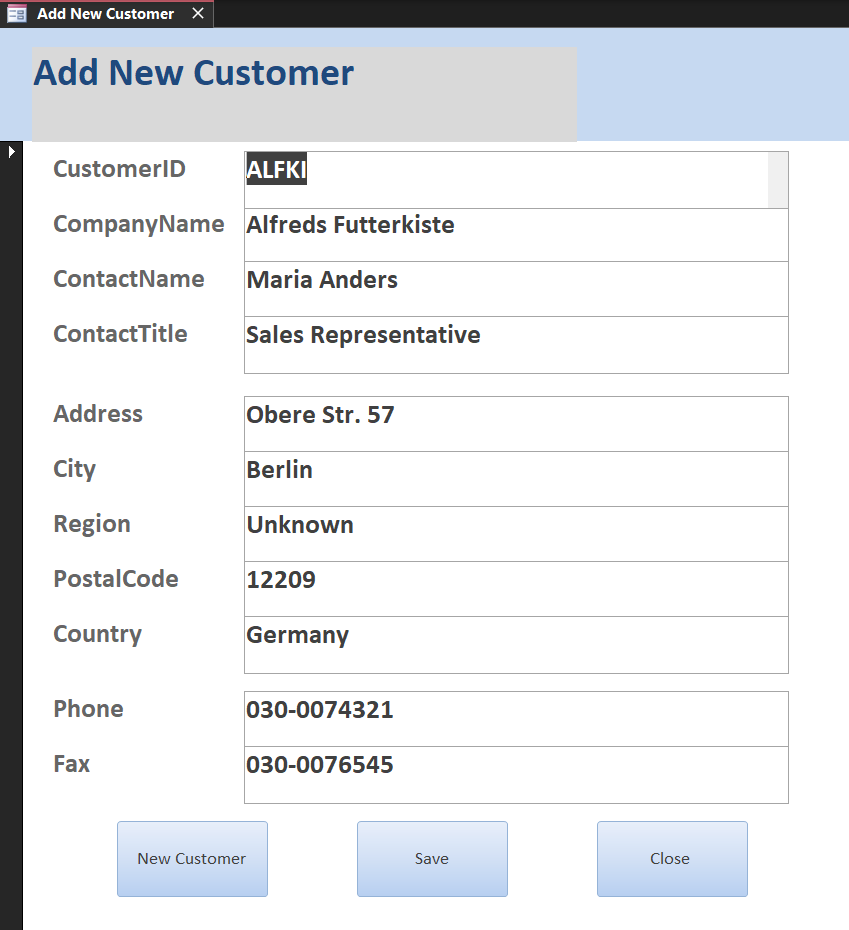
\includegraphics[width=0.7\linewidth,
		height=0.5\textheight]{phase3_5.png}
		\caption{فرم ثبت مشتری جدید }
		\label{fig:phase3_5}
	\end{figure}
	
	در ادامه فرآیند توسعه، فرم ثبت سفارش‌های جدید\LTRfootnote{New Order Form} به عنوان یکی از پیچیده‌ترین بخش‌های سیستم پیاده‌سازی شد؛ چرا که ثبت هر سفارش مستلزم برقراری ارتباط همزمان میان موجودیت‌های متعددی نظیر مشتریان، کارمندان و اقلام کالا است. ساختار این بخش به صورت یک فرم اصلی\LTRfootnote{Main Form} متصل به جدول سفارش‌ها و یک فرم فرعی\LTRfootnote{Order Details Subform} با عنوان جزئیات سفارش‌ها پیاده‌سازی گردید که از طریق فیلد کلید خارجی شناسه سفارش\LTRfootnote{OrderID} به یکدیگر پیوند داده شده‌اند. جهت تضمین صحت ورود داده‌ها و جلوگیری از بروز خطاهای مرجع، برای انتخاب کارمند و مشتری از جعبه‌های ترکیبی\LTRfootnote{Combo Boxes} استفاده شد که اطلاعات خود را به صورت پویا از جداول مرجع فراخوانی می‌کنند. به منظور افزایش سرعت کاربری، فیلدهای مربوط به مشخصات ارسال کالا به گونه‌ای پیکربندی شدند که به محض انتخاب مشتری، اطلاعات نشانی وی به صورت پیش‌فرض در فیلدهای مربوطه درج شود، هرچند امکان ویرایش دستی این فیلدها برای ارسال به مقاصد متفاوت نیز وجود دارد. در این فرم، محاسبات مالی به صورت کاملاً پویا پیاده‌سازی گردید؛ به طوری که در فرم فرعی، یک کنترل محاسباتی\LTRfootnote{Calculated Control} با عنوان جمع ردیف\LTRfootnote{LineTotal} با فرمول ضرب قیمت واحد در تعداد پس از کسر تخفیف، جمع هر قلم کالا را مشخص می‌سازد (مانند محاسبه مبلغ ۱۶۸ دلار برای ۱۲ عدد از یک کالای\lr{Queso Cabrales} با قیمت واحد ۱۴ دلار و تخفیف صفر درصد). در نهایت، در فرم اصلی با بهره‌گیری از فرمول محاسباتی ریاضی به صورت:
\begin{center}
	\begin{latin}
		\footnotesize
		\texttt{Order Total = Sum([UnitPrice] * [Quantity] * (1 - [Discount])) + Nz([Freight])}
	\end{latin}
	\end{center}
	0 جمع کل فاکتور\LTRfootnote{Order Total} با احتساب هزینه حمل‌ونقل محاسبه می‌گردد که در سفارش نمونه شماره ۱۰۲۴۸، مقدار نهایی پس از جمع مبالغ اقلام و هزینه حمل ۳۲.۳۸ دلاری، معادل ۴۷۲.۳۸ دلار در فیلد مربوطه منعکس شده است.
	
	\begin{figure}[H]
		\centering
		% به جای picture5.png نام عکس واقعی خود را قرار دهید
		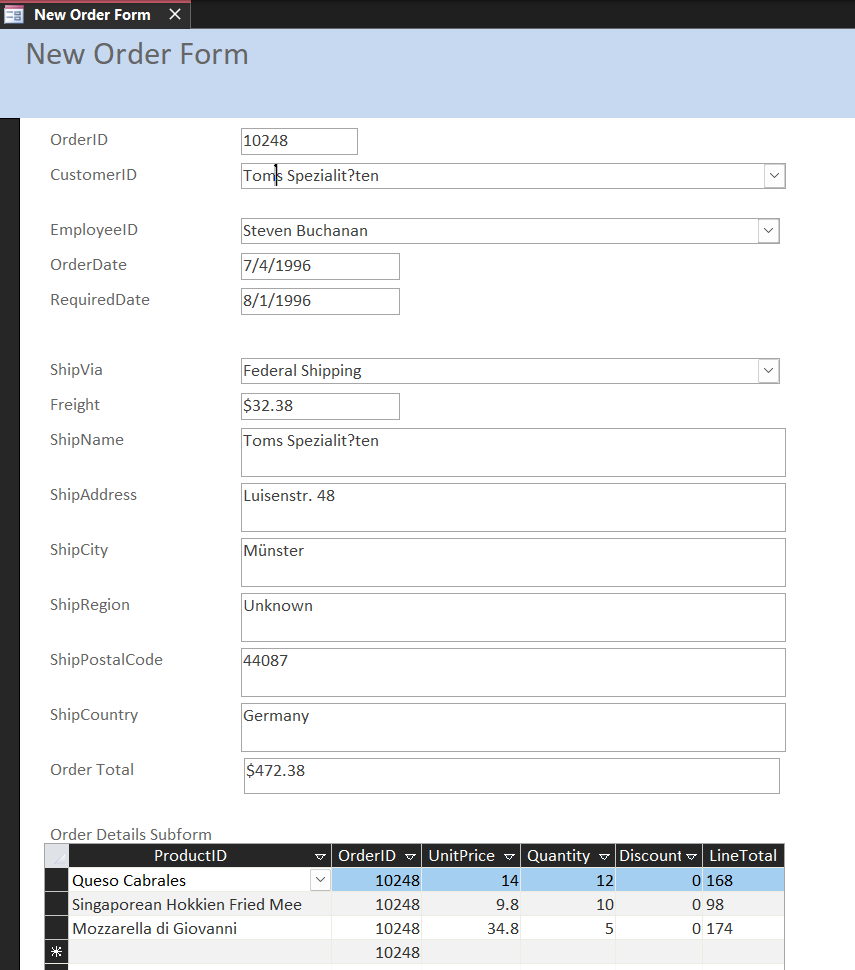
\includegraphics[width=0.7\linewidth,
		height=0.4\textheight]{phase3_6.png}
		\caption{ فیلد های فرم ثبت سفارش جدید}
		\label{fig:phase3_6}
	\end{figure}
	
	به منظور مدیریت پویای عملیات روی سفارش‌ها، مجموعه‌ای از دکمه‌های کنترلی کلیدی شامل ثبت سفارش جدید\LTRfootnote{New Order}، ذخیره سفارش\LTRfootnote{Save Order}، حذف سفارش\LTRfootnote{Delete Order} و چاپ فاکتور\LTRfootnote{Print Invoice} در قالب یک نوار ابزار اختصاصی طراحی و در فرم سفارش‌ها ادغام شد تا دسترسی کاربر به فرآیندهای سیستمی به بهینه‌ترین شکل ممکن برقرار گردد.
	
	\begin{figure}[H]
		\centering
		% به جای picture5.png نام عکس واقعی خود را قرار دهید
		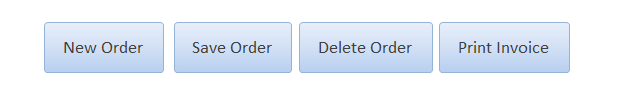
\includegraphics[width=0.8\linewidth,
		height=0.3\textheight,
		keepaspectratio]{phase3_7.png}
		\caption{ایجاد قابلیت و دکمه پرینت فاکتور برای سفارش}
		\label{fig:phase3_7}
	\end{figure}
	
	
	بخش پایانی این فاز به طراحی قابلیت چاپ فاکتور فروش اختصاصی اختصاص یافت تا امکان ارائه خروجی رسمی به مشتریان فراهم گردد. بدین منظور، ابتدا گزارشی\LTRfootnote{Report} تحت عنوان فاکتور\LTRfootnote{Invoice} طراحی شد که اطلاعات خود را از ادغام جداول مختلف استخراج کرده و ساختاری استاندارد شامل شناسه سفارش، تاریخ، نام مشتری، تلفن، نام محصول، تعداد، قیمت واحد، درصد تخفیف، جمع ردیف، هزینه حمل و نقل و جمع کل سفارش را نمایش می‌دهد. این گزارش در حالت پیش‌فرض تمام اسناد ثبت‌شده در سیستم (نظیر سفارش‌های شماره ۱۰۲۴۸، ۱۰۲۴۹ و ۱۰۲۵۰) را به صورت متوالی و گروه‌بندی شده نمایش می‌دهد.
	
	\begin{figure}[H]
		\centering
		% به جای picture5.png نام عکس واقعی خود را قرار دهید
		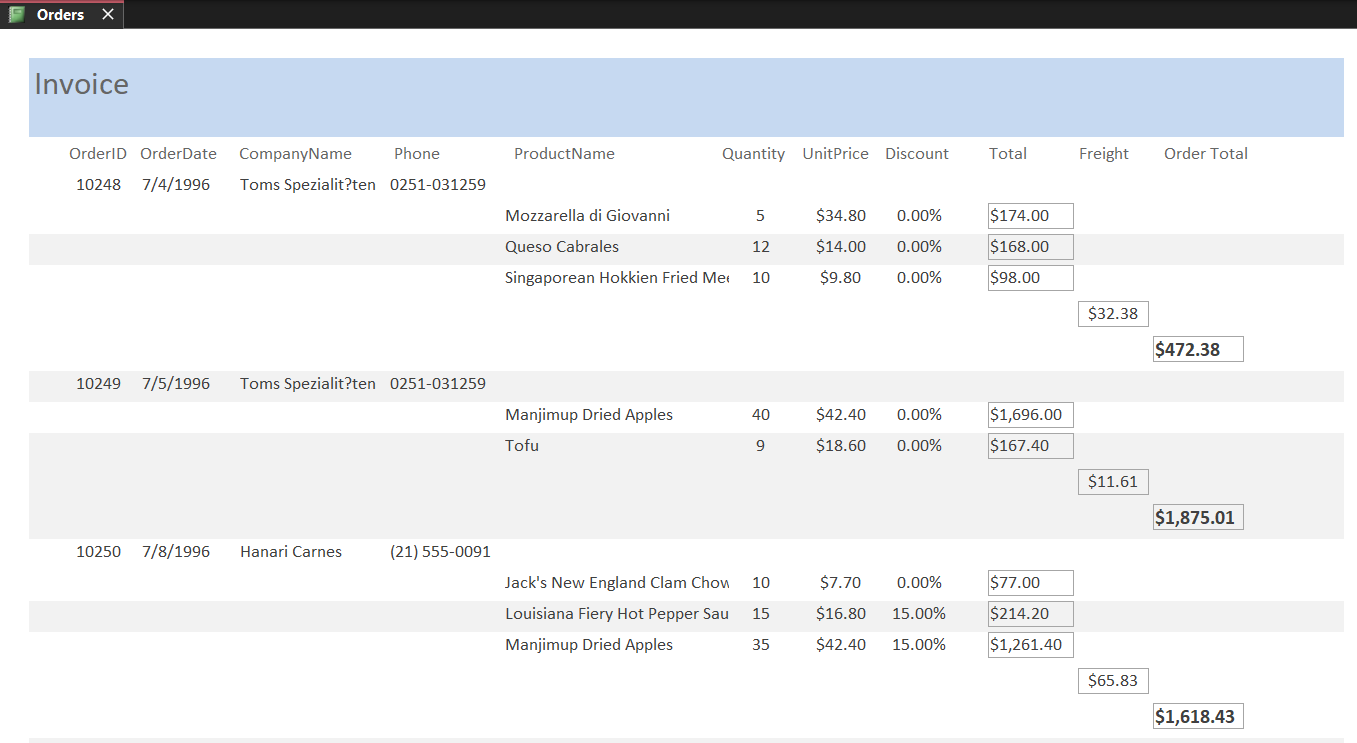
\includegraphics[width=1\linewidth,
		height=1\textheight,
		keepaspectratio]{phase3_8.png}
		\caption{ایجاد گزارش فاکتور، شامل فاکتور تمام سفارش ها}
		\label{fig:phase3_8}
	\end{figure}
	
	چالش اصلی در این بخش، فیلتر کردن هوشمند گزارش بر اساس سفارشی بود که کاربر در لحظه روی فرم ثبت سفارش مشاهده می‌کند. برای حل این مسئله، ماکروی ویژه‌ای برای دکمه چاپ سفارش تعریف شد که با اعمال شرط فیلتر\LTRfootnote{Where Condition} به صورت \texttt{\lr{[OrderID]=[Forms]![Orders]![OrderID]}} موتور پایگاه داده را ملزم می‌سازد تا گزارش خروجی را دقیقاً منطبق بر شناسه فاکتور فعال در فرم (برای نمونه سفارش شماره ۱۰۲۴۸) فیلتر کرده و خروجی تک‌صفحه‌ای اختصاصی آن را جهت چاپ آماده سازد. این رویکرد ساختاریافته علاوه بر افزایش سرعت عمل کاربران سیستم، به طور کامل مانع از بروز تداخل اطلاعاتی در فرآیندهای مالی می‌گردد.
	
	\begin{figure}[H]
		\centering
		% به جای picture5.png نام عکس واقعی خود را قرار دهید
		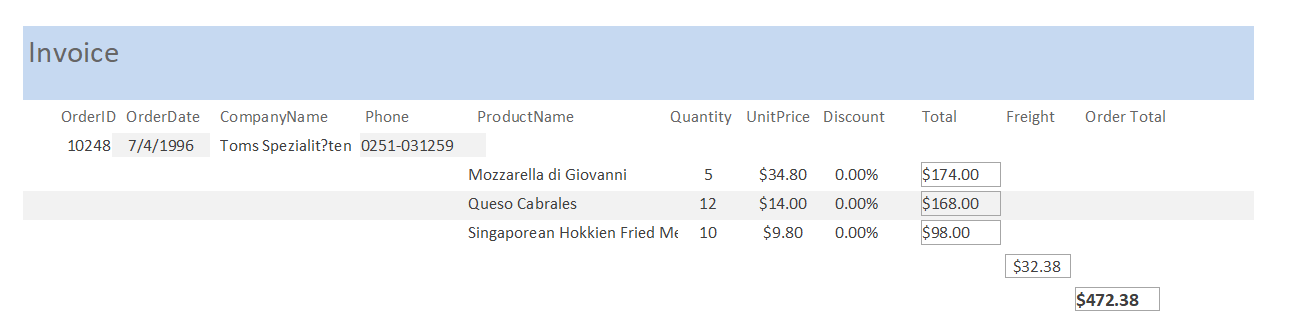
\includegraphics[width=1\linewidth,]{phase3_9.png}
		\caption{فاکتور ایجاد شده برای سفارش 10248}
		\label{fig:phase3_9}
	\end{figure}
	
	
	
	\subsection{طراحی گزارش‌های مدیریتی و تحلیلی}
	
	\subsubsection{گزارش عملکرد و ارزش‌گذاری گروه‌های کالایی}
	
	در فرآیند طراحی سیستم گزارش‌دهی جهت ارزیابی عملکرد گروه‌های کالایی، رویکرد چندمرحله‌ای در طراحی پرس‌وجوها\LTRfootnote{Multi-stage Queries} به عنوان استراتژی اصلی برگزیده شد تا علاوه بر تضمین دقت در محاسبات پیچیده، کارایی سیستم در مواجهه با حجم بالای داده‌ها حفظ گردد. در گام نخست، با هدف سنجش تنوع محصولات، پرس‌وجوی اختصاصی جهت اتصال جداول دسته‌بندی و محصولات طراحی شد که در آن با بهره‌گیری از تابع شمارش بر روی شناسه کالا\LTRfootnote{CountProductID}، میزان تنوع محصولات در هر گروه استخراج گردید. در گام دوم، برای سنجش دقیق میزان فروش، پرس‌وجوی دیگری با پیوند جداول دسته‌بندی، کالاها و جزئیات سفارشات ایجاد شد تا مجموع درآمد خالص هر گروه با استفاده از تابع محاسباتی زیر در قالب ارز\LTRfootnote{Currency} تعیین گردد:
	
	\begin{center}
		\begin{latin}
			\small
			\texttt{SalesAmount: CCur(Sum([UnitPrice] * [Quantity] * (1 - [Discount])))}
		\end{latin}
	\end{center}
	
	این خروجی با اعمال ترتیب نزولی\LTRfootnote{Descending} تنظیم گردید تا گروه‌های پیشرو در سودآوری در اولویت نمایش قرار گیرند. در نهایت، با ادغام این زیرمجموعه‌ها در یک پرس‌وجوی جامع، بستری برای تغذیه ابزارهای تحلیل بصری فراهم شد.
	
	\begin{figure}[H]
		\centering
		
		% تصویر سمت راست
		\begin{minipage}{0.48\textwidth}
			\centering
			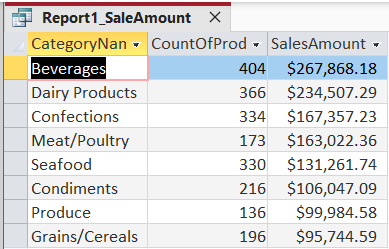
\includegraphics[width=1\linewidth,
			height=0.3\textheight,
			keepaspectratio]{phase3_10.png}
			\caption{خروجی مجموع فروش گروه ها}
			\label{fig:hase3_10}
		\end{minipage}
		\hfill % ایجاد فاصله بین دو تصویر
		% تصویر سمت چپ
		\begin{minipage}{0.48\textwidth}
			\centering
			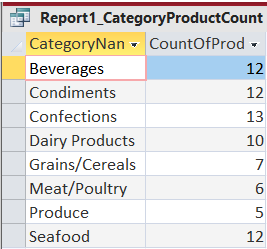
\includegraphics[width=1\linewidth,
			height=0.2\textheight,keepaspectratio]{phase3_11.png}
			\caption{خروجی  تنوع گروه ها}
			\label{fig:phase3_11}
		\end{minipage}
		
	\end{figure}
	
	\begin{figure}[H]
		\centering
		% به جای picture5.png نام عکس واقعی خود را قرار دهید
		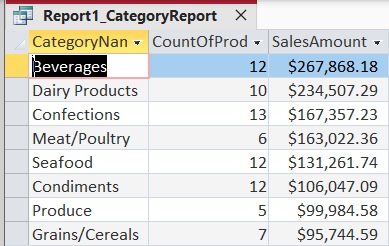
\includegraphics[width=1\linewidth,height=0.2\textheight,keepaspectratio]{phase3_12.png}
		\caption{ تجمیع دو خروجی}
		\label{fig:phase3_12}
	\end{figure}
	
	برای نمایش بهینه این داده‌ها، دو نوع نمودار با رویکردهای مدیریتی متفاوت طراحی گردید؛ نمودار نخست که به صورت ستونی ساده\LTRfootnote{Column Chart} پیاده‌سازی شده است، با نمایش مستقیم سهم هر گروه از کل درآمد، امکان شناسایی سریع دسته‌های پربازده نظیر نوشیدنی‌ها\LTRfootnote{Beverages} و لبنیات\LTRfootnote{Dairy Products} را فراهم می‌آورد. در مقابل، نمودار دوم که یک نمودار ترکیبی دو محوره\LTRfootnote{Dual-Axis Combo Chart} است، با هدف کشف رابطه استراتژیک میان تنوع کالا و بازدهی مالی طراحی شده است. در این نمودار، میزان فروش بر روی ستون‌های محور اصلی و تعداد کالاها به صورت خطی بر روی محور ثانویه ترسیم شده است. تحلیل این ساختار ترکیبی حقایق مدیریتی مهمی را آشکار می‌سازد؛ به عنوان نمونه، مشاهده می‌شود که برخی دسته‌ها مانند شیرینی‌جات\LTRfootnote{Confections} با وجود دارا بودن بیشترین تنوع کالایی، در رتبه سوم فروش قرار دارند، در حالی که دسته لبنیات با تنوع کمتر، بازدهی مالی بالاتری ثبت کرده است. این تحلیل بصری به مدیران زنجیره تأمین اجازه می‌دهد تا به جای افزایش بی‌رویه تنوع کالا، بر بهینه‌سازی سبد محصولات پرتقاضا تمرکز نموده و از انباشت سرمایه در بخش‌های کم‌بازده جلوگیری کنند.
	
	
		\begin{figure}[H]
		\centering
		
		% تصویر سمت راست
		\begin{minipage}{0.48\textwidth}
			\centering
			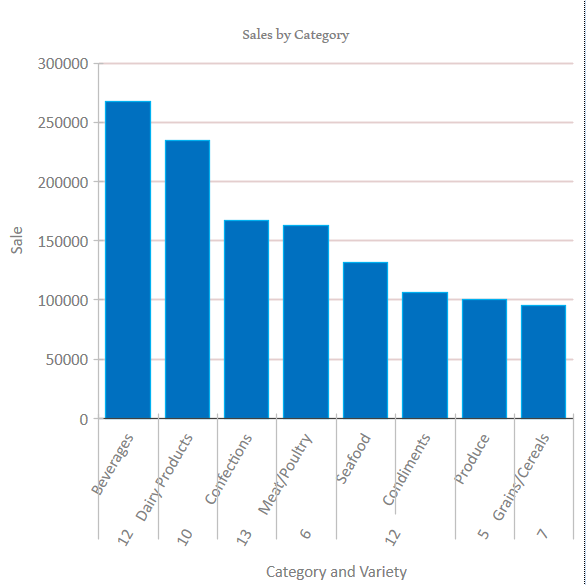
\includegraphics[width=1\linewidth,
			height=0.3\textheight,
			keepaspectratio]{phase3_13.png}
			\caption{نمایش نمودار مجموع فروش هر گروها}
			\label{fig:hase3_13}
		\end{minipage}
		\hfill % ایجاد فاصله بین دو تصویر
		% تصویر سمت چپ
		\begin{minipage}{0.48\textwidth}
			\centering
			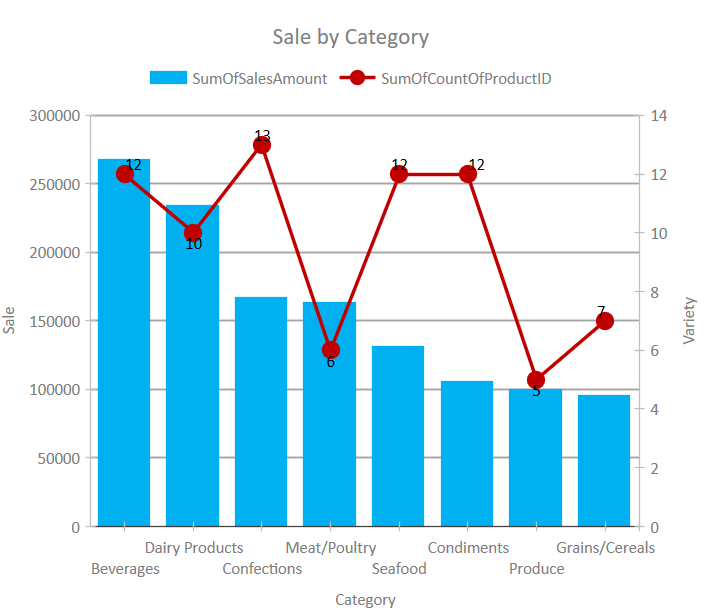
\includegraphics[width=1\linewidth,
			height=0.3\textheight,keepaspectratio]{phase3_14.png}
			\caption{نمایش نمودار تحلیلی تاثیر تنوع بر میزان فروش هر گروه}
			\label{fig:phase3_14}
		\end{minipage}
		
	\end{figure}
	
	\subsubsection{گزارش تحلیل رفتار خرید مشتریان}
	
	ارزیابی مستمر رفتار مشتریان و شناسایی مخاطبان کلیدی، نقشی حیاتی در بهینه‌سازی زنجیره عرضه و اجرای موفق طرح‌های بازاریابی هدفمند\LTRfootnote{Targeted Marketing} ایفا می‌کند. به منظور تحلیل دقیق رفتار خرید مشتریان از دو جنبه حجم مبادلات مالی و تعداد دفعات سفارش، یک معماری اطلاعاتی چندلایه در پایگاه داده طراحی گردید. فرآیند پیاده‌سازی با طراحی پرس‌وجوی پایه با عنوان {\small\lr{Report2\_CustomersListOnTotalPurchase}} آغاز شد که طی آن، پیوند میان جداول مشتریان، سفارش‌ها و جزئیات سفارش‌ها از طریق فیلدهای کلیدی شناسه مشتری و شناسه سفارش\LTRfootnote{OrderID} برقرار گردید تا امکان ردیابی کل فرآیند خرید از مشخصات خریدار تا جزئی‌ترین اقلام سبد کالا فراهم شود. در ساختار این پرس‌وجو، شناسه مشتری مبنای گروه‌بندی قرار گرفت و حجم کل خرید هر مشتری با اعمال فرمول محاسباتی زیر بر روی قیمت واحد، تعداد و اعمال درصد تخفیف استخراج شد:
	
	\begin{center}
		\begin{latin}
			\small
			\texttt{TotalPurchase = Sum(CCur([UnitPrice] * [Quantity] * (1 - [Discount])))}
		\end{latin}
	\end{center}
	
	این فیلد محاسباتی با اعمال ساختار مرتب‌سازی نزولی\LTRfootnote{Descending} تنظیم گردید تا مشتریان استراتژیک در صدر فهرست قرار گیرند. هم‌زمان، فراوانی سفارش‌های هر مشتری با استفاده از تابع \lr{Count(OrderID)} محاسبه شد و پس از صحت‌سنجی خروجی جهت اطمینان از عدم وجود رکوردهای تکراری، گزارش مدیریتی اصلی با نام \lr{rpt\_TopCustomers} طراحی گردید. برای تسهیل تصمیم‌گیری‌های مدیریتی، در سطح طراحی این گزارش و نه در سطح پرس‌وجو، از قابلیت قالب‌بندی شرطی\LTRfootnote{Conditional Formatting} بهره گرفته شد؛ به طوری که ارزش‌های خرید فراتر از ۵۰,۰۰۰ با رنگ سبز و مقادیر کمتر از ۱۰,۰۰۰ با رنگ قرمز برجسته شدند تا مشتریان کلیدی و مشتریان با پتانسیل خرید پایین بلافاصله قابل تفکیک باشند.
	
	\begin{figure}[H]
		\centering
		
		% تصویر سمت راست
		\begin{minipage}{0.4\textwidth}
			\centering
			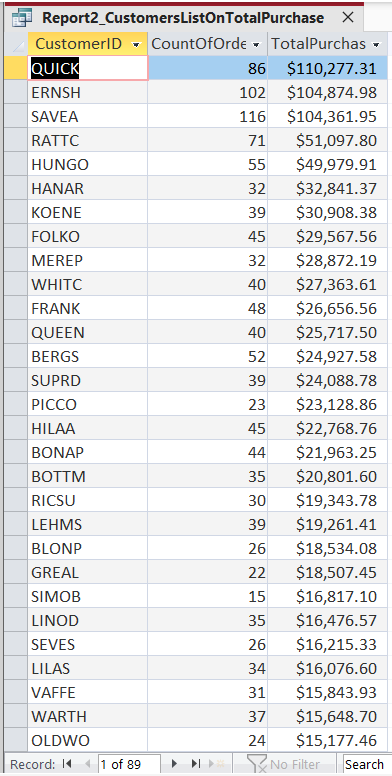
\includegraphics[width=1\linewidth,
			height=0.35\textheight,
			keepaspectratio]{phase3_15.png}
			\caption{خروجی به ترتیب مجموع خرید مشتریان }
			\label{fig:hase3_15}
		\end{minipage}
		\hfill % ایجاد فاصله بین دو تصویر
		% تصویر سمت چپ
		\begin{minipage}{0.58\textwidth}
			\centering
			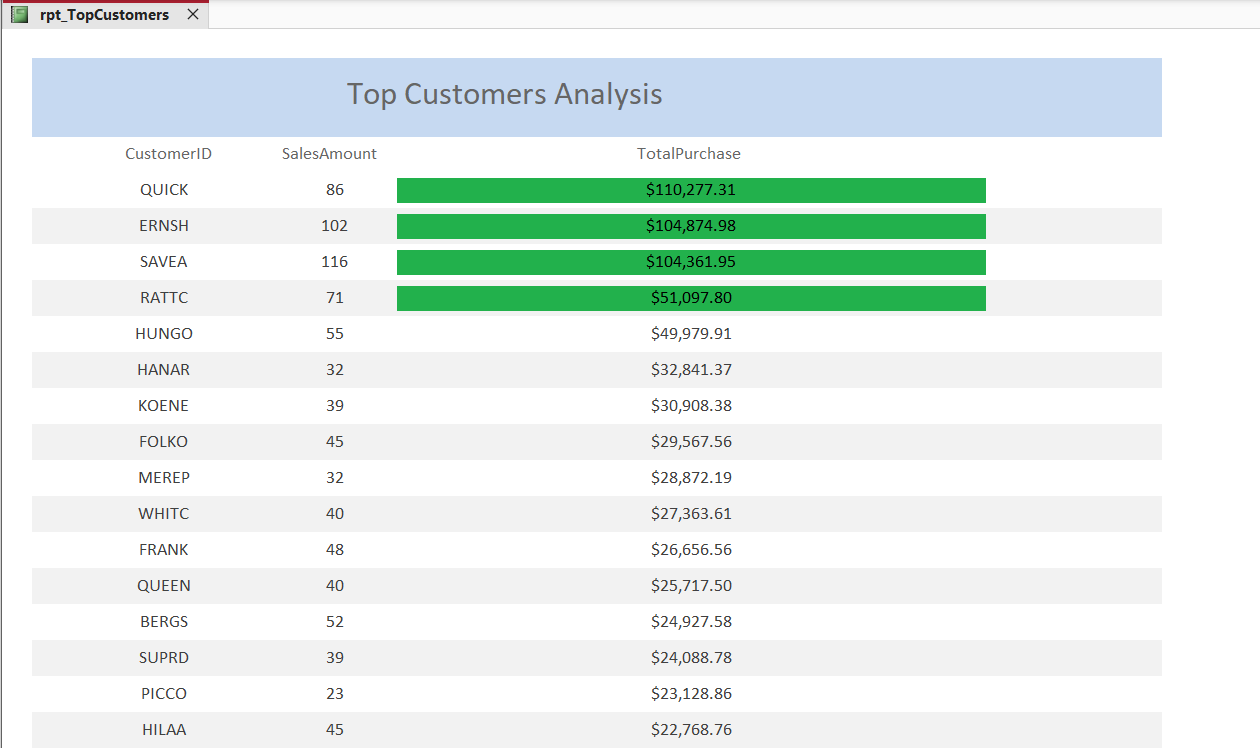
\includegraphics[width=1\linewidth,
			height=0.3\textheight]{phase3_16.png}
			\caption{ نمایی از گزارش تهیه شده براساس مجموع خرید مشتریان }
			\label{fig:phase3_16}
		\end{minipage}
		
	\end{figure}
	
	
	در گام بعدی و برای تکمیل این زنجیره تحلیلی، پرس‌وجو و گزارش موازی دیگری با تمرکز بر تعداد دفعات خرید توسعه یافت تا مشتریان وفادار\LTRfootnote{Frequent Buyers} شناسایی شوند. در این بخش، منطق گروه‌بندی مجدداً بر روی شناسه مشتری اعمال و شمارش سفارش‌ها با تابع \lr{Count(OrderID)} انجام شد. گزارش حاصل از این تحلیل نیز مجهز به قالب‌بندی شرطی گردید که در آن مشتریانی با بیش از ۵۰ سفارش با رنگ سبز و مشتریانی با کمتر از ۱۰ سفارش با رنگ قرمز نمایش داده شدند.
	
	
	
	\begin{figure}[H]
		\centering
		
		% تصویر سمت راست
		\begin{minipage}{0.4\textwidth}
			\centering
			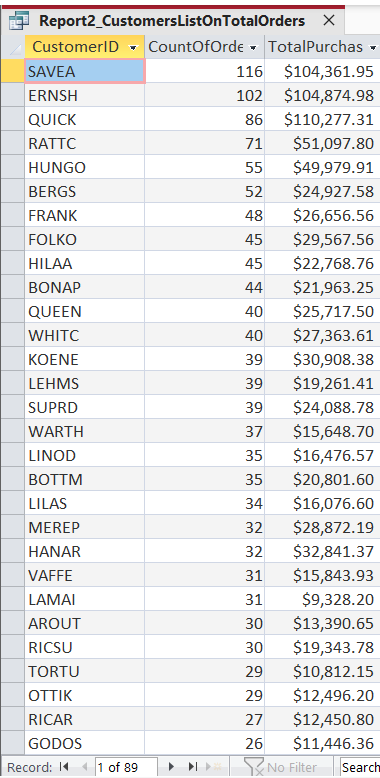
\includegraphics[width=1\linewidth,
			height=0.3\textheight,
			keepaspectratio]{phase3_17.png}
			\caption{خروجی به ترتیب مجموع خرید مشتریان }
			\label{fig:hase3_17}
		\end{minipage}
		\hfill % ایجاد فاصله بین دو تصویر
		% تصویر سمت چپ
		\begin{minipage}{0.58\textwidth}
			\centering
			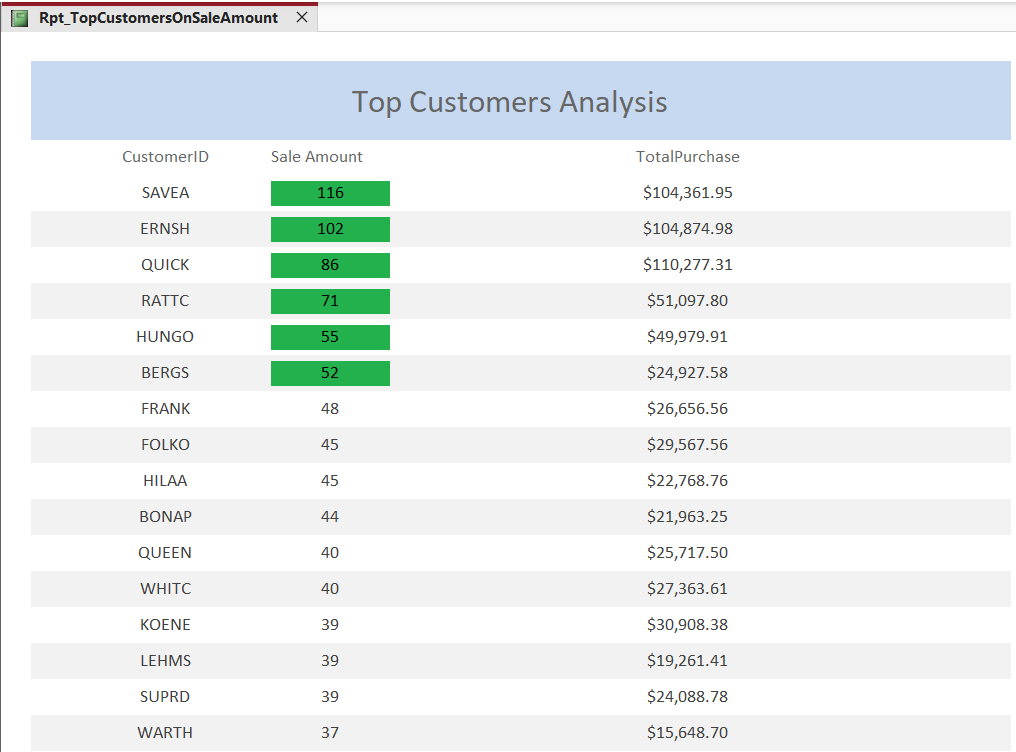
\includegraphics[width=1\linewidth,
			height=0.3\textheight]{phase3_18.png}
			\caption{ نمایی از گزارش تهیه شده براساس مجموع خرید مشتریان }
			\label{fig:phase3_18}
		\end{minipage}
	\end{figure}
		
	در ادامه و به‌منظور تکمیل چارچوب تحلیلی رفتار مشتریان، دو گزارش مکمل دیگر نیز طراحی و پیاده‌سازی گردید. گزارش نخست به شناسایی ۱۰ درصد برتر مشتریان از نظر میزان خرید اختصاص یافت؛ به این صورت که مشتریان بر مبنای فیلد \lr{TotalPurchase} به‌صورت نزولی رتبه‌بندی شده و با استفاده از قابلیت \lr{Top Values} در سطح پرس‌وجو، تنها مشتریانی که در بالاترین دهک ارزش خرید قرار داشتند استخراج شدند. منطق این گزارش بر آن استوار است که بهره‌گیری از یک معیار نسبی به‌جای یک آستانه ثابت مالی، دقت بیشتری در شناسایی مشتریان کلیدی فراهم می‌آورد؛ زیرا در این روش، انتخاب مشتریان برتر متناسب با توزیع واقعی داده‌ها و ساختار خرید در جامعه مشتریان انجام می‌شود. این رویکرد از منظر بازاریابی، برای طراحی کمپین‌های هدفمند، تخصیص بهینه مشوق‌های فروش، شناسایی مشتریان با ارزش بالا و تمرکز بر مشتریان دارای بیشترین ظرفیت سودآوری، اهمیت ویژه‌ای دارد.
	
	همچنین، پرس‌وجو و گزارش مستقلی نیز برای استخراج ۱۰ درصد برتر مشتریان از نظر تعداد دفعات خرید طراحی گردید تا مشتریان وفادار و دارای تکرار خرید بالا با دقت بیشتری شناسایی شوند. در این گزارش، مبنای رتبه‌بندی بر اساس فیلد شمارشی سفارش‌ها یعنی \lr{Count(OrderID)} قرار گرفت و با اعمال منطق \lr{Top Values}، تنها مشتریانی انتخاب شدند که از نظر دفعات مراجعه و تکرار خرید در بالاترین سطح قرار داشتند. ضرورت طراحی این گزارش از آن جهت است که در بسیاری از سناریوهای بازار، فراوانی خرید لزوماً با ارزش ریالی خرید یکسان نیست و ممکن است مشتریانی با سفارش‌های متعدد، نقش مهم‌تری در پایداری تقاضا، گردش مستمر فروش و اثربخشی برنامه‌های وفادارسازی ایفا کنند. از این رو، این گزارش به‌عنوان ابزاری مکمل برای اجرای کمپین‌های نگهداشت مشتری، ارائه پیشنهادهای دوره‌ای، طراحی طرح‌های وفاداری و تحلیل رفتار مشتریان پرتکرار مورد استفاده قرار می‌گیرد.
	
	
	\begin{figure}[H]
		\centering
		
		% تصویر سمت راست
		\begin{minipage}{0.48\textwidth}
			\centering
			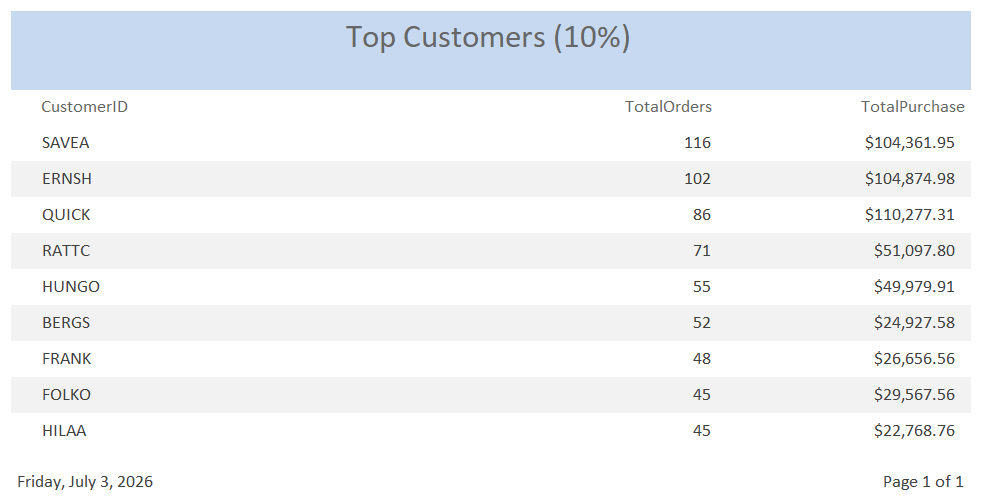
\includegraphics[width=1\linewidth,
			height=0.4\textheight,
			keepaspectratio]{phase3_19.png}
			\caption{ 10 درصد برتر مشتریان از لحاظ تعداد خرید }
			\label{fig:hase3_19}
		\end{minipage}
		\hfill % ایجاد فاصله بین دو تصویر
		% تصویر سمت چپ
		\begin{minipage}{0.48\textwidth}
			\centering
			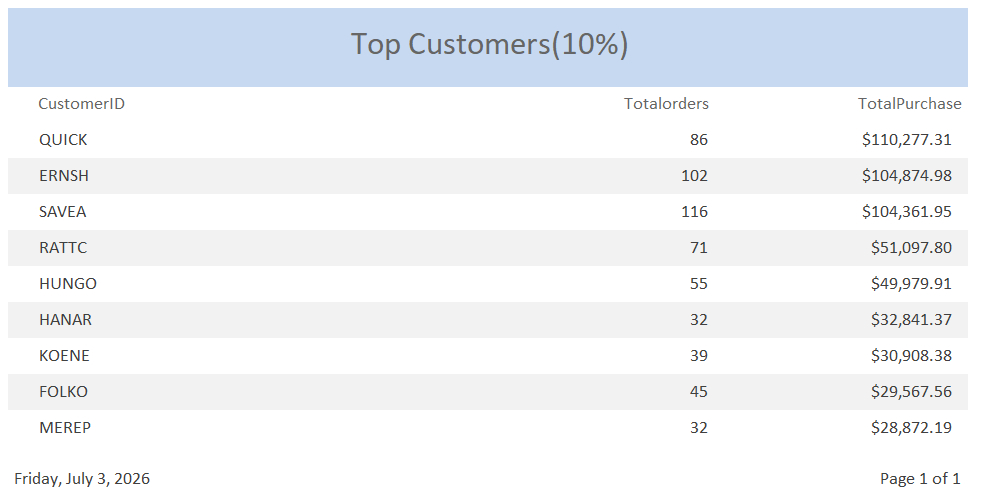
\includegraphics[width=1\linewidth,
			height=0.15\textheight]{phase3_20.png}
			\caption{  10 درصد برتر مشتریان  از لحاظ میزان خرید }
			\label{fig:phase3_20}
		\end{minipage}
	\end{figure}
	
\end{document}
